%%%%%%%%%%%%%%%%%%%%%%%%%%%%%%%%%%%%%%%%%%%%%%%
%%%     Declarations (skip to Begin Document, line 88, for parts you fill in)
%%%%%%%%%%%%%%%%%%%%%%%%%%%%%%%%%%%%%%%%%%%%%%%

%%\documentclass[10pt]{article}
%%\documentclass[10pt]{report}
\documentclass[letterpaper]{article}
\usepackage{geometry}
%\usepackage{xcolor}
\usepackage[table]{xcolor}
\usepackage{amsmath}
\usepackage[some]{background}
%\usepackage{lipsum}
%\usepackage{natbib}
\usepackage{siunitx}

% C I T A T I O N S
\usepackage[backend=biber, style=apa]{biblatex}  
%\usepackage{biblatex} 
\addbibresource{paperpile.bib}

\usepackage[hidelinks]{hyperref}

% C A P T I O N S
%\usepackage{caption, copyrightbox}
%\captionsetup{justification=centering, labelfont=sc, labelsep=endash}

% Tables
\usepackage{float}
\usepackage[utf8]{inputenc}
\usepackage{tabularx}
\usepackage{booktabs}
\usepackage{longtable}

\usepackage{diagbox} %table split headers
\usepackage{longtable}
\usepackage{array}
\usepackage{rotating}
\usepackage{eqparbox}
\usepackage{makecell, caption, booktabs}

% Stuff needed to get table to span pages
\usepackage{enumitem}
%\usepackage{array, booktabs, longtable}
\newcolumntype{x}[1]{>{\raggedright}p{#1}}

\usepackage{etoolbox}
\AtBeginEnvironment{longtable}{%
    \setlist[itemize]{nosep,     % <-- new list setup
                      topsep     = 0pt       ,
                      partopsep  = 0pt       ,
                      leftmargin = *         ,
                      label      = $\bullet$ ,
                      before     = \vspace{-\baselineskip},
                      after      = \vspace{-0.5\baselineskip}
                        }
                           }% end of AtBeginEnvironment
% End table span
% Listings
\usepackage{listings}

\usepackage{geometry}  % Lots of layout options.  See http://en.wikibooks.org/wiki/LaTeX/Page_Layout
\geometry{letterpaper}  % ... or a4paper or a5paper or ... 
\usepackage{fullpage}  % somewhat standardized smaller margins (around an inch)
\usepackage{setspace}  % control line spacing in latex documents
\usepackage[parfill]{parskip}  % Activate to begin paragraphs with an empty line rather than an indent

\usepackage{amsmath,amssymb}  % latex math
\usepackage{empheq} % http://www.ctan.org/pkg/empheq
\usepackage{bm,upgreek}  % allows you to write bold greek letters (upper & lower case)

% for typsetting algorithm pseudocode see http://en.wikibooks.org/wiki/LaTeX/Algorithms_and_Pseudocode
\usepackage{algorithmic,algorithm}  

\usepackage{graphicx}  % inclusion of graphics; see: http://en.wikibooks.org/wiki/LaTeX/Importing_Graphics
% allow easy inclusion of .tif, .png graphics
\DeclareGraphicsRule{.tif}{png}{.png}{`convert #1 `dirname #1`/`basename #1 .tif`.png}

% \usepackage{subfigure}  % allows subfigures in figure
\usepackage{caption}
\usepackage{subcaption}

\usepackage{xspace}
\newcommand{\latex}{\LaTeX\xspace}

\usepackage{color}  % http://en.wikibooks.org/wiki/LaTeX/Colors

\long\def\todo#1{{\color{red}{\bf TODO: #1}}}

\long\def\ans#1{{\color{blue}{\em #1}}}
\long\def\ansnem#1{{\color{blue}#1}}
\long\def\boldred#1{{\color{red}{\bf #1}}}
\long\def\boldred#1{\textcolor{red}{\bf #1}}
\long\def\boldblue#1{\textcolor{blue}{\bf #1}}

% Useful package for syntax highlighting of specific code (such as python) -- see below
\usepackage{listings}  % http://en.wikibooks.org/wiki/LaTeX/Packages/Listings
\usepackage{textcomp}


%%% The following lines set up using the listings package
\renewcommand{\lstlistlistingname}{Code Listings}
\renewcommand{\lstlistingname}{Code Listing}

%%% Specific for python listings
\definecolor{gray}{gray}{0.5}
\definecolor{green}{rgb}{0,0.5,0}

\lstnewenvironment{python}[1][]{
\lstset{
language=python,
basicstyle=\footnotesize,  % could also use this -- a little larger \ttfamily\small\setstretch{1},
stringstyle=\color{red},
showstringspaces=false,
alsoletter={1234567890},
otherkeywords={\ , \}, \{},
keywordstyle=\color{blue},
emph={access,and,break,class,continue,def,del,elif ,else,%
except,exec,finally,for,from,global,if,import,in,i s,%
lambda,not,or,pass,print,raise,return,try,while},
emphstyle=\color{black}\bfseries,
emph={[2]True, False, None, self},
emphstyle=[2]\color{green},
emph={[3]from, import, as},
emphstyle=[3]\color{blue},
upquote=true,
morecomment=[s]{"""}{"""},
commentstyle=\color{gray}\slshape,
emph={[4]1, 2, 3, 4, 5, 6, 7, 8, 9, 0},
emphstyle=[4]\color{blue},
literate=*{:}{{\textcolor{blue}:}}{1}%
{=}{{\textcolor{blue}=}}{1}%
{-}{{\textcolor{blue}-}}{1}%
{+}{{\textcolor{blue}+}}{1}%
{*}{{\textcolor{blue}*}}{1}%
{!}{{\textcolor{blue}!}}{1}%
{(}{{\textcolor{blue}(}}{1}%
{)}{{\textcolor{blue})}}{1}%
{[}{{\textcolor{blue}[}}{1}%
{]}{{\textcolor{blue}]}}{1}%
{<}{{\textcolor{blue}<}}{1}%
{>}{{\textcolor{blue}>}}{1},%
%framexleftmargin=1mm, framextopmargin=1mm, frame=shadowbox, rulesepcolor=\color{blue},#1
framexleftmargin=1mm, framextopmargin=1mm, frame=single,#1
}}{}
%%% End python code listing definitions

\DeclareMathOperator{\diag}{diag}
\DeclareMathOperator{\cov}{cov}


%\bibliography{./paperpile.bib}
\author{Evan McGinnis}
\title{Automated Weeding}



\definecolor{titlepagecolor}{cmyk}{1,.60,0,.40}

\DeclareFixedFont{\bigsf}{T1}{phv}{b}{n}{1.5cm}

\backgroundsetup{
scale=1,
angle=0,
opacity=1,
contents={\begin{tikzpicture}[remember picture,overlay]
 \path [fill=titlepagecolor] (-0.5\paperwidth,5) rectangle (0.5\paperwidth,10);  
\end{tikzpicture}}
}
\makeatletter                       
\def\printauthor{%                  
    {\large \@author}}              
\makeatother
\author{%
    Evan McGinnis \\
    Graduate Student \\
    Biosystems Analytics \\
    \texttt{evanmc@arizona.edu}\vspace{40pt} \\
    }
\begin{document}
\begin{titlepage}
\BgThispage
\newgeometry{left=1cm,right=4cm}
\vspace*{1cm}
\noindent
%%\vspace*{0.4\textheight}
\textcolor{white}{\Huge\textbf{\textsf{Image segmentation under field conditions}}}
\vspace*{3.5cm}\par
\noindent
\begin{minipage}{0.35\linewidth}
    \begin{flushright}
        \printauthor
    \end{flushright}
\end{minipage} \hspace{15pt}
%
\begin{minipage}{0.02\linewidth}
    \rule{1pt}{175pt}
\end{minipage} \hspace{-10pt}
%
\begin{minipage}{0.70\linewidth}
\vspace{5pt}
    \begin{abstract} 
This paper presents an overview of image segmentation under field conditions with ambient lighting. Discussed are index-based techniques using visible light using the RGB color space (Triangular Greenness, Normalized Difference, Excess Green, Excess Red, Color of Vegetation Extraction, Excess Green - Excess Red, Normalize Green-Red Difference, Vegetative, Combined Index I and II, and Modified Excess Green), using color spaces other than RGB (CIELab, YCbCr, and YIQ), and classification-based where each pixel is classified using machine-learning techniques (Multi-layer Perceptron, Linear Discriminant Analysis, and Support Vector Machine). While index-based approaches proved to be the most practical, as classification based approaches tended to require more computation resources than are typically available under field conditions, index-based approaches often had significant errors that should be taken into account when selecting an approach. The index with the highest overall error rate was NGRDI, with 11.65\% of pixels mis-identified. An approach using the YIQ color space achieved the lowest error rate, with 1.4\%.
    \end{abstract}
\end{minipage}
\end{titlepage}
\restoregeometry
%
% F R O N T  M A T T E R
%
\tableofcontents
\listoffigures
\listoftables
%\listofequations
\newpage

%
% O V E R V I E W 
%



\section{Introduction}
Agricultural images of crops taken from an overhead perspective typically contain only two things: crop and ground.  Images taken for tasks such as navigation tend to often include other features -- most notably, the horizon -- as they are acquired more parallel to the ground. While there may be things on the ground that must be ignored (irrigation equipment, ground debris, rocks), the goal of image segmentation remains unchanged: plants are retained in the final image, and everything else discarded. This document will discuss this process considering only visible light data using three techniques: index-based (the vegetated pixels are exaggerated and isolated from the background), Non-RGB colorspace thresholding (images in colorspaces such as YIQ are processed), and  classification-based (the pixels are classified as vegetation or ground).  Image segmentation is often a first step in image processing, as doing so reduces the information content of an image for subsequent processing.  For example, it provides little value in a vegetation treatment system to classify a pebble on the ground as such -- that information can be safely discarded as the first step in image processing. The subsequent processing may be positive, applying an enhancement or treatment to vegetation identified as crop, or negative, applying a chemical, mechanical, or directed energy (i.e., laser) treatment to eliminate vegetation identified as weeds. This document will treat image segmentation as a preprocessing step in an overall workflow.

\section{Methdology}
Images were taken at the University of Arizona's Maricopa Agricultural Center (MAC) located in Maricopa, AZ (N 33.061857, E 111.967145) of a cantaloupe planting in May 2024. Images were obtained using an Apple IPhone 8, using ambient lighting. These images were color corrected using values obtained from images taken under identical lighting conditions of a Datacolor Sypder correction chart.  Images obtained using other sources are used to illustrate techniques or points, but most of the analysis shown in this document are from the set gathered at the MAC. All processing software was written in Python 3 and data analysis written in R.  
\section{Techniques}
\subsection{Index Based}
Index-based approaches follow the same basic workflow: a mask is produced from the original image and then applied to that image, retaining vegetated pixels, while discarding non-vegetated pixels. Figure~\ref{fig:segmentation} demonstrates an example of this process. starting with an image acquired under field conditions. The resulting image can be subsequently processed with the knowledge that all remaining pixels in the image are plants.

\begin{figure}[H]
	\centering
	\begin{subfigure}[h]{.30\textwidth}
	  \centering
	  \includegraphics[width=1\linewidth]{figures/original.jpg}
	  \caption{Field view of lettuce and weed}
	  \label{fig:original}
	\end{subfigure}
	\begin{subfigure}[h]{.30\textwidth}
	  \centering
	  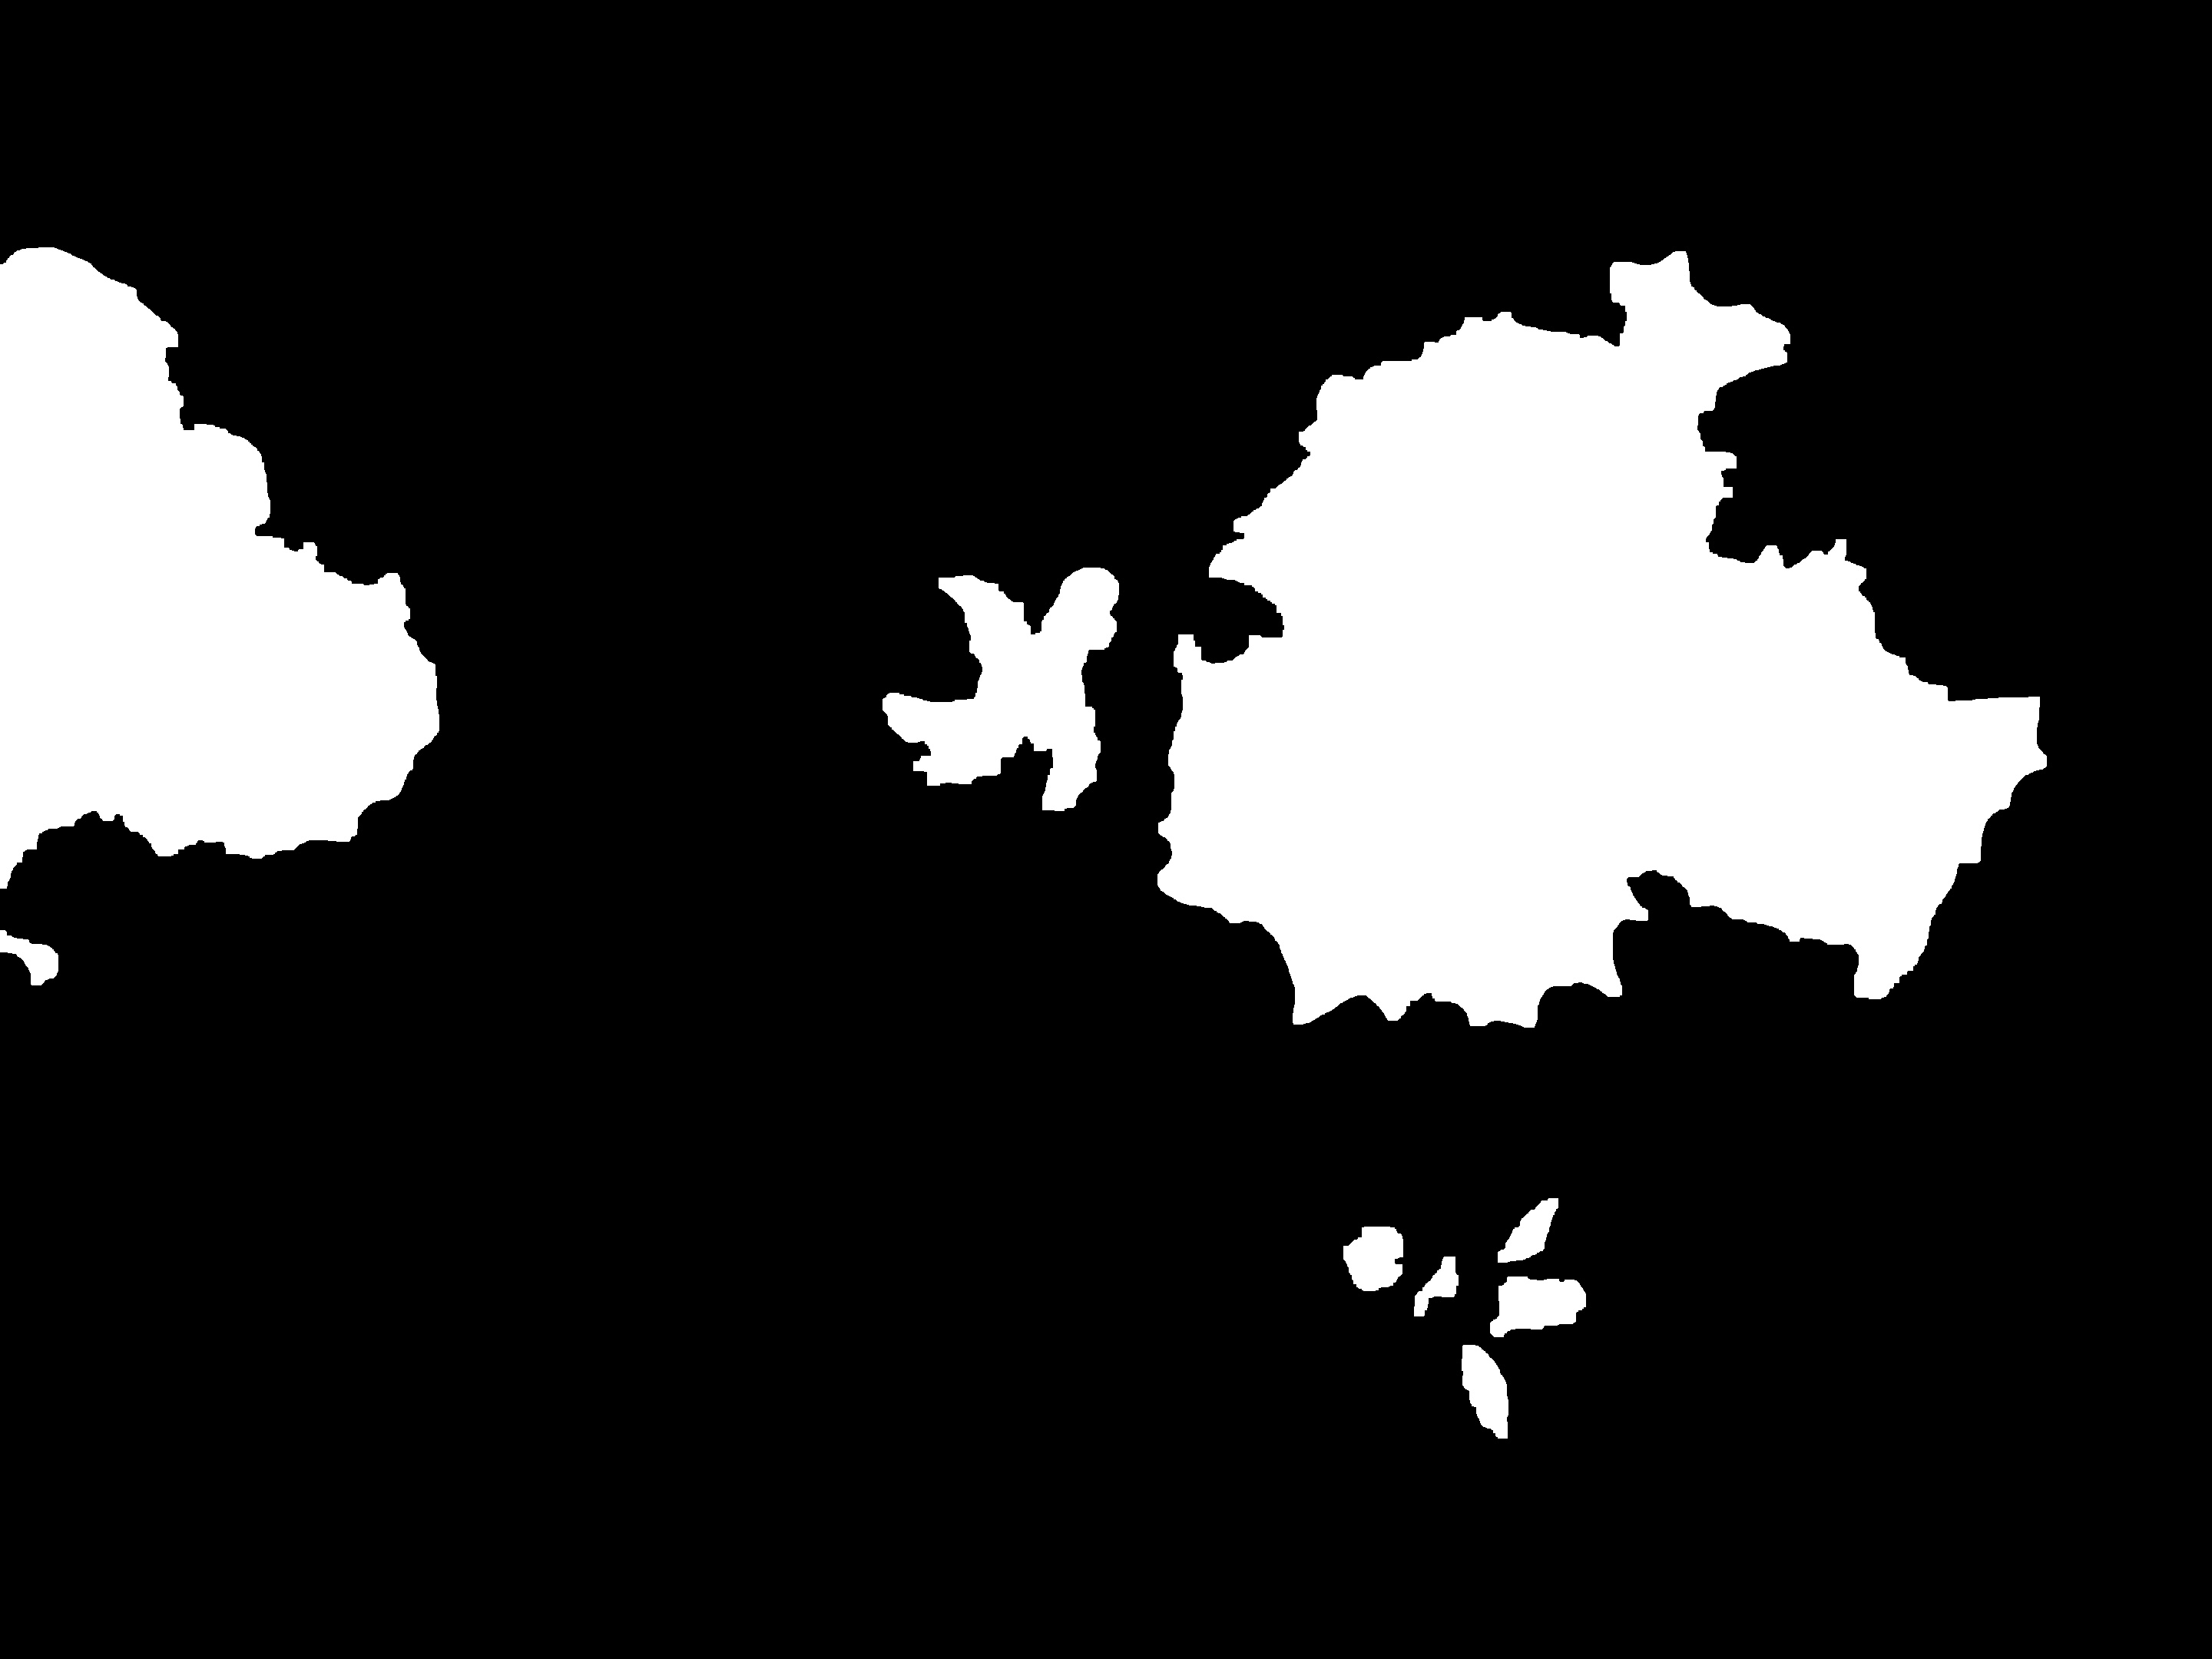
\includegraphics[width=1\linewidth]{figures/original-mask.jpg}
	  \caption{Mask produced with NDI}
	  \label{fig:mask}
	\end{subfigure}
	\begin{subfigure}[h]{.30\textwidth}
	  \centering
	  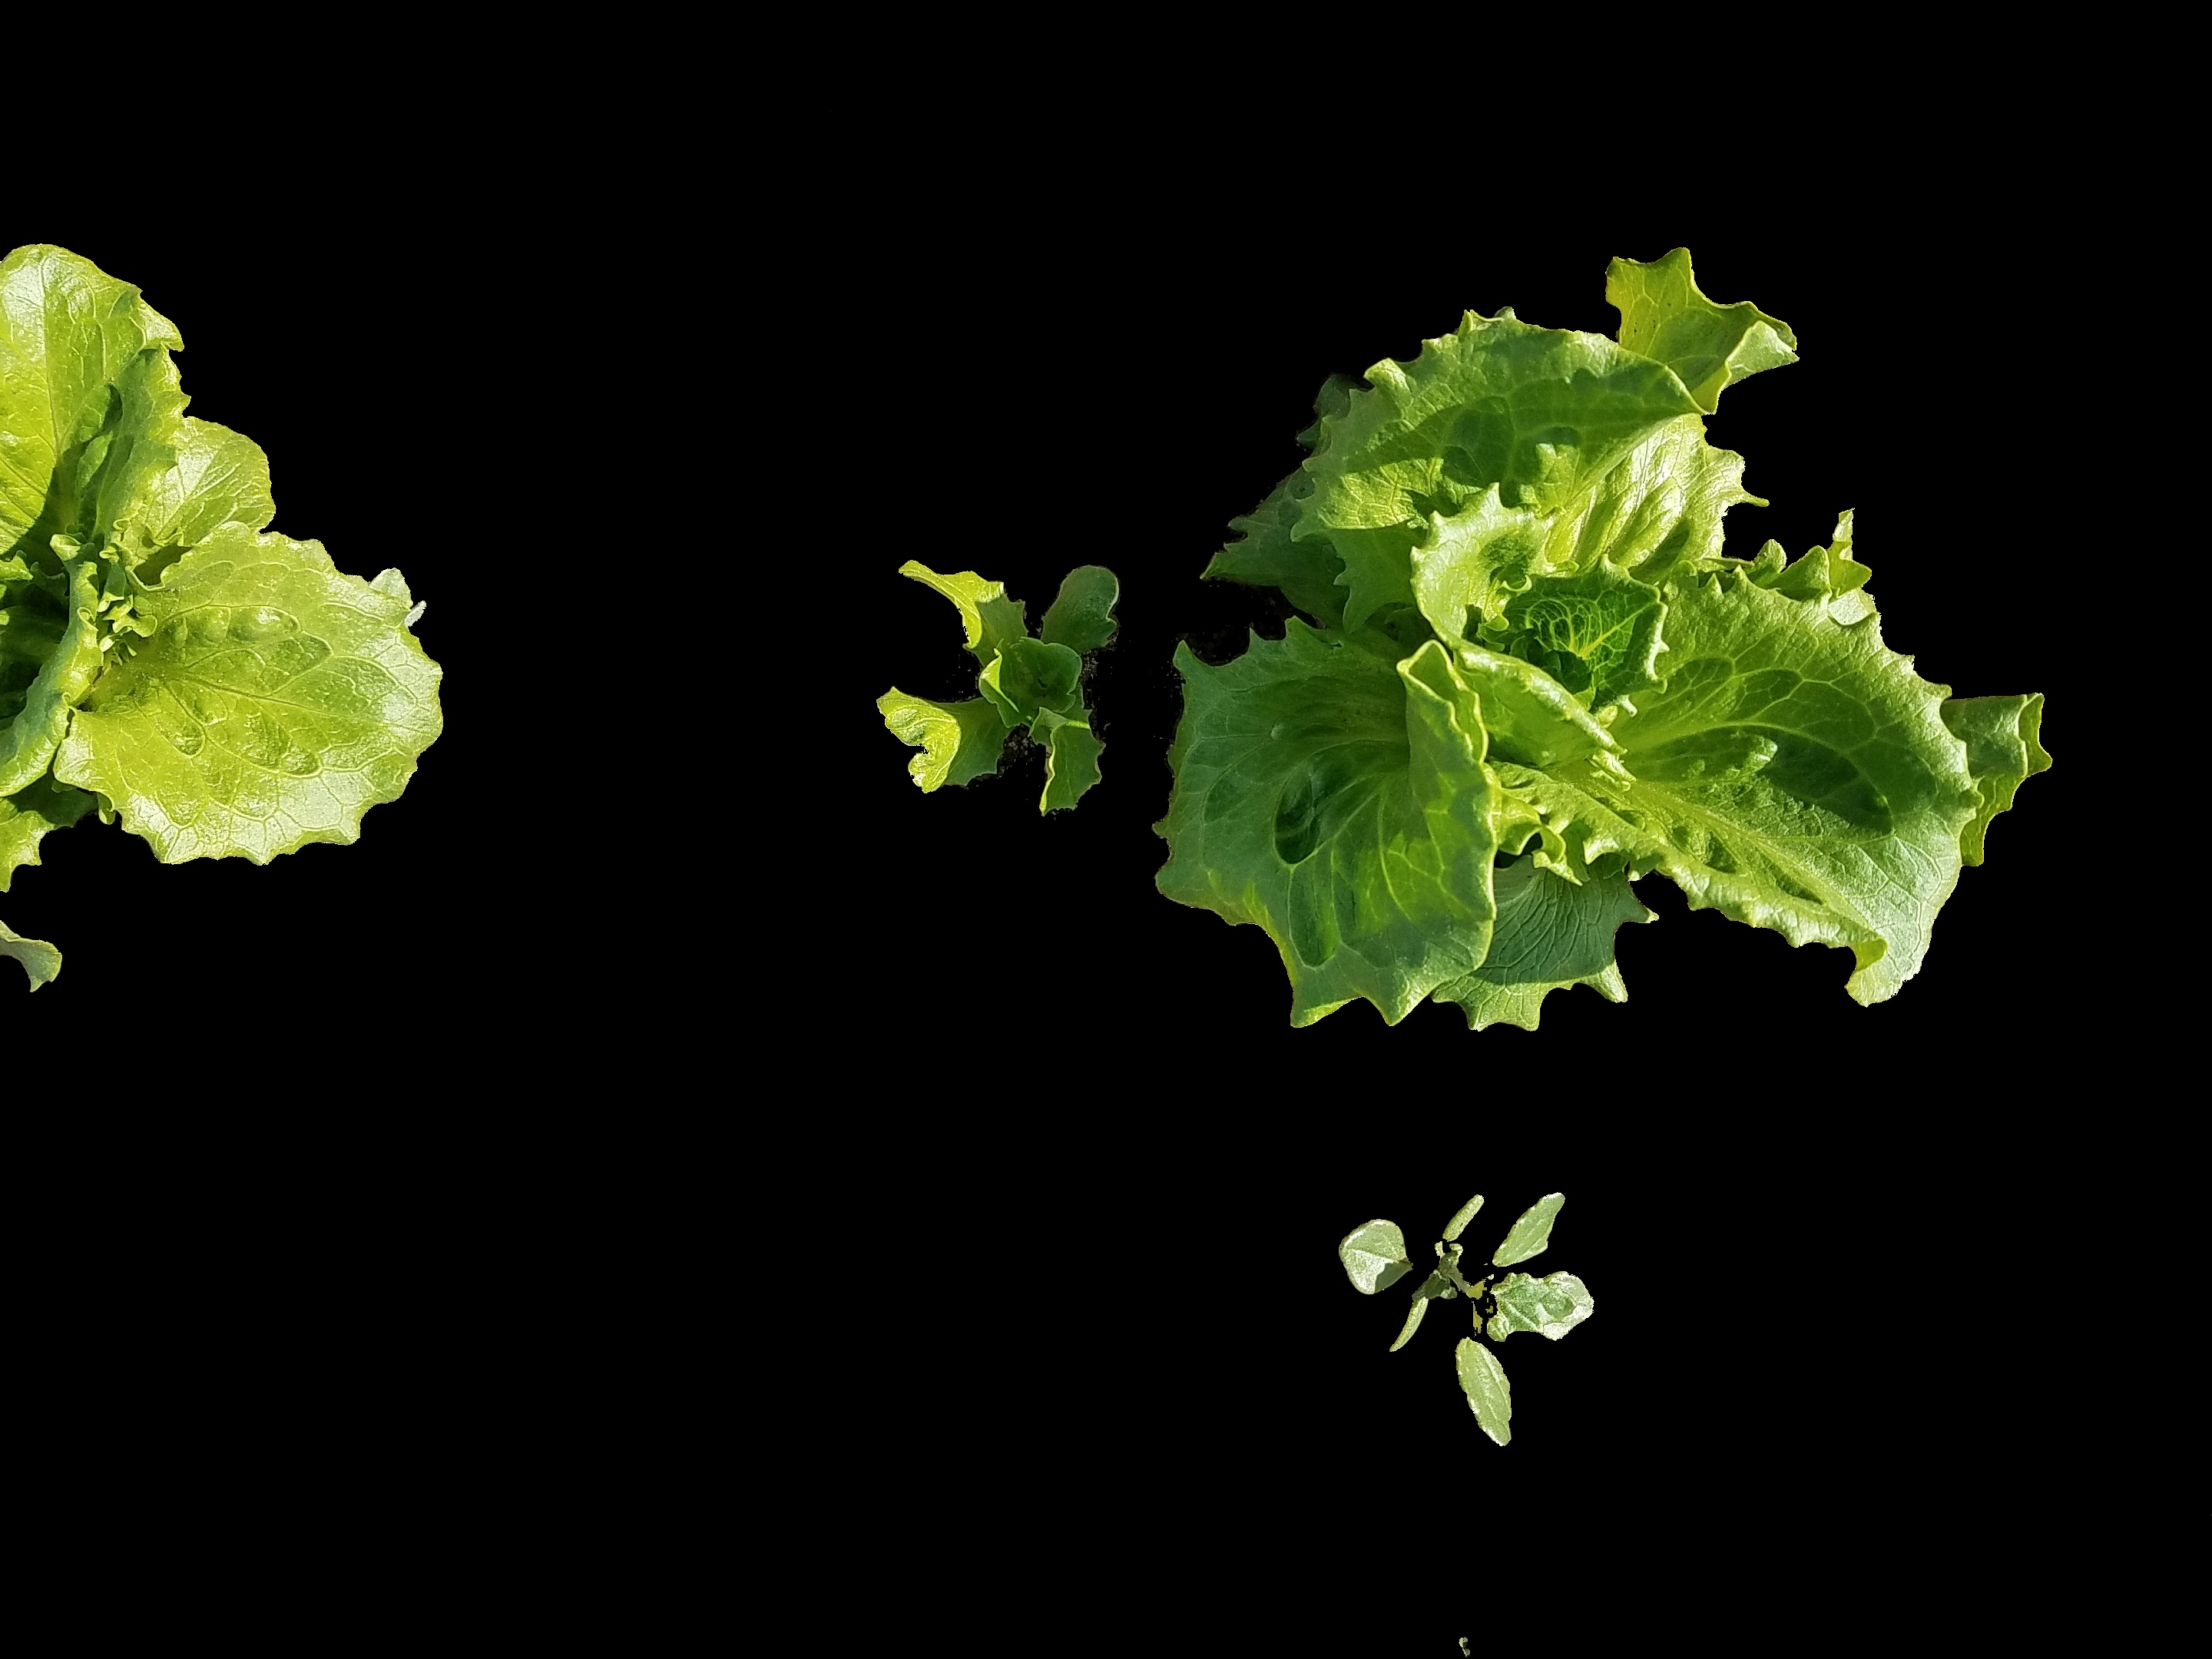
\includegraphics[width=1\linewidth]{figures/original-masked.jpg}
	  \caption{After applying mask}
	  \label{fig:original-masked}
	\end{subfigure}
	\caption[Before and after segmentation]{Before and after segmentation. Note the absence of the stems seen in the weed in the lower portion of~\ref{fig:original-masked} -- this is made a bit more obvious with a close examination of the mask shown in~\ref{fig:mask}.  This is an example of one of the shortcomings of some of the index based approaches that will be discussed in Section~\ref{section:problems-color}. The stems of the weed are not sufficiently green ``enough'' to register as vegetation.}
	\label{fig:segmentation}
\end{figure}

\subsubsection{RGB}
This commonly-encountered colorspace is often the only color space representation available from consumer cameras (dedicated or embedded within a phone), although machine vision cameras often can be configured to capture images in other spaces. This space is a fairly simple encoding of the amounts of Red, Green, and Blue of a pixel. A \textit{vegetation index} is used that exaggerates the bands typically associated with vegetation while minimizing non-vegetated bands.

These indices are used to create a mask that is then applied to the original source image to permit vegetation to show while masking details that are not relevant (ground pixels, stones, and other items that may appear in field conditions) The intent here is to remove all pixels that are not vegetated while leaving the vegetated pixels unmanipulated. The formulae for various RGB indices are shown in Table~\ref{table:segmentation}.

% Spacing between the rows
{\renewcommand{\arraystretch}{1.1}%

{
% This avoids the document line spacing affecting the contents of the table
\setstretch{1.0}
% Example to span two pages
\begin{longtable}{x{\dimexpr.25\columnwidth-2\tabcolsep}
                  x{\dimexpr.35\columnwidth-2\tabcolsep}
                  x{\dimexpr.4\columnwidth-2\tabcolsep}}
	%\begin{hyphenrules}{nohyphenation}
	\caption{Visible light indices} \label{tab:example}  \\
	\toprule
		{\textbf{Index}} & {\textbf{Formula}} & {\textbf{Abbreviation \& Source}}
		\tabularnewline
		\midrule
		    \endfirsthead
		%%%%
		    \caption{Visible light indices (cont.)}\label{tab:example}  \\
	\toprule
	{\textbf{Index}} & {\textbf{Formula}} & {\textbf{Abbreviation \& Source}}
	\tabularnewline
	\midrule
	    \endhead
	%%%%
	\midrule[\heavyrulewidth]
	\multicolumn{3}{r}{\footnotesize\itshape
	                   Continued on the next page}
	    \endfoot
	%%%%
	\bottomrule
	    \endlastfoot
	%%%%
			Triangular Greenness
			& \begin{minipage}[t]{0.3\textwidth}
				$R_{green} - \alpha R_{red} - \beta R_{blue}\\ \alpha = \frac {2(\lambda_{blue} - \lambda_{green})} {(\lambda_{blue} - \lambda_{red})}\\ 
			    	\beta = \frac {2(\lambda_{green} - \lambda_{red})} {(\lambda_{blue} - \lambda_{red})} $
			   \end{minipage}     
			& TGI - \parencite{Hunt2013-ih}
	\tabularnewline\addlinespace
	
			Normalized Difference     
			& $128 * \left( \left( \frac {(G - R)} {(G + R)} \right) + 1 \right) $                    
			& NDI - \parencite{Woebbecke1995-bw}
	\tabularnewline\addlinespace
	
			Excess Green      
			& \begin{minipage}[t]{0.3\textwidth}
				$R = \frac {R} {R_{max}}\\ G = \frac {G} {G_{max}}\\ B = \frac {B} {B_{max}}$ 
			   \end{minipage}
			& ExG - \parencite{Woebbecke1995-yg} 
	\tabularnewline\addlinespace
	
			Excess Red      
			& $1.3 R - G$ 
			& ExR - \parencite{Meyer1999-zn}
	\tabularnewline\addlinespace
	
			Color Index of Vegetation Extraction      
			& $0.441 R - 0.811 G + 0.385 B + 18.78745$
			& CIVE - \parencite{Kataoka2003-pu}
	\tabularnewline\addlinespace
	
			Excess Green - Excess Red   
			& $ExG - ExR$ 
			& ExGExR - \parencite{Neto2004-od}
	\tabularnewline\addlinespace
	
			Normalized Green-Red Difference    
			& $\frac {(G - R)} {(G + R)}$ 
			& NGRDI - \parencite{Hunt2005-tz}
	\tabularnewline\addlinespace
	
			Vegetative Index      
			& $\frac {G} {R^aB^{(1-a)}}, a = 0.667$ 
			& VEG - \parencite{Hague2006-da}
	\tabularnewline\addlinespace
	
			Combined Indices 1   
			& $ExG + CIVE + ExGR + VEG$ 
			& COM1 - \parencite{Guijarro2011-bl}
	\tabularnewline\addlinespace
	
			Modified Excess Green      
			& $1.262G - 0.884R - 0.311B$ 
			& MExG - \parencite{Burgos-Artizzu2011-od}
	\tabularnewline\addlinespace
	
			Combined Indices 2      
			& $0.36ExG + 0.47CIVE + 0.17VEG$ 
			&  COM2 - \parencite{Guerrero2012-zi}
	%\tabularnewline\addlinespace
	\label{table:segmentation}
\end{longtable}
}


The creation of an index has produced data that often exaggerates portions of the image with vegetated pixels, but deciding what portions of the data to discard and which to keep can be automated instead of using a single threshold for all images. The manual selection of a threshold can be shown to work relatively well, and can be fine-tuned by examining the results ensure that the number of vegetated pixels are maximized, while the number of non-vegetated pixels are minimized (in other words, we do not want to have significant portions of the ground in the image, but we do want as much of the plant as is possible. Unfortunately, images can be acquired under different lighting conditions, leading to the case where there is often not a threshold that works well for all images. An alternative, first proposed by \citeauthor*{Otsu1979-io}  \parencite{Otsu1979-io}, is to select this threshold automatically for each image, or the image can be selected using the \textit{Triangle} algorithm.

\begin{figure}[H]
	\centering
	\begin{subfigure}[h]{.48\textwidth}
	  \centering
	  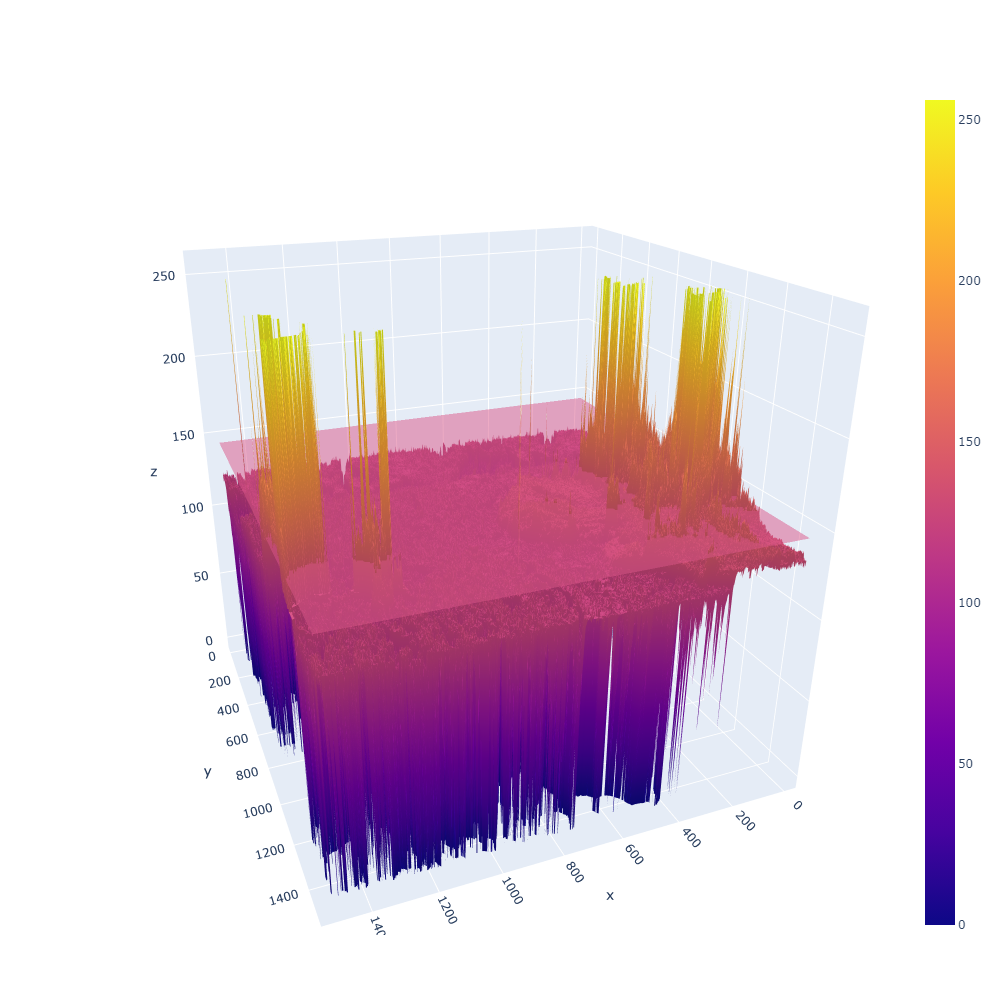
\includegraphics[height=5cm]{./figures/ndi-1-of-2.png}
	  \caption{Image segmented using NDI}
	  \label{fig:ndi-1}
	\end{subfigure}
	\hfill
	\begin{subfigure}[h]{.48\textwidth}
	  \centering
	  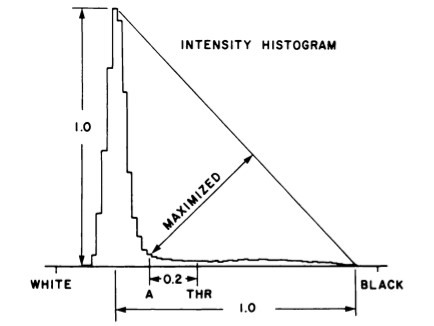
\includegraphics[height=5cm]{./figures/triangle-algorithm}
	  \caption{Triangle method for threshold selection.}
	  \label{fig:ndi-2}
	\end{subfigure}
	\caption[NDI segmentation and threshold selection]{An example of NDI segmentation and threshold selection. A threshold for the production of a mask can be done manually, perhaps by selecting all values below 140 (noted by the translucent pink plane in \ref{fig:ndi-1}) to form the mask that will be applied to the image, illustrated by the semi-opaque plane. While that manual selection may be sufficient to perform the segmentation of an image set acquired under the same ambient conditions, it may lead to the exclusion of portions of the plant in images taken under different conditions. Using the Triangle algorithm \parencite{Brink1996-xy,Zack1977-yl} allows this selection to be made automatically. The point at which the line between the lowest and highest points in the histogram is selected as the threshold, selecting a threshold applicable to each image in a set rather than a global value used for all images in a set.}
	\label{fig:ndi-segmentation}
\end{figure}

\subsubsection{HSI and HSV}
The Hue, Saturation and Intensity (HSI) and Hue Saturation and Value (HSV) color spaces present an opportunity to consider how saturated the colors are instead of just emphasizing the green found it an image. While that is a bit of an over-simplification of basing a technique on the values found within the RGB bands, it is essentially what is happening. Hue based approaches take much the same approach in one respect -- the hue frequently present in vegetation (green) is represented as peaking around $120^o$ in both models. This is convenient, certainly, as simply considering points as vegetation of they contain hue values around the peak. How wide this range is, of course, will determine what is captured. And while the topic of color is revisited in Section ~\ref{section:problems-color}, consider that leaves contain much that is not green, just as the ground contains much that is not brown. A leaf may contain hue values in the range of 40-70, an indication that the hue is toward the red end of the representation. Likewise, a patch of dirt may contain hue values in the range of 15-20, an indication that the hue is much more red than anything else. HSV is a bit more complicated, in that the V band should be normalized between $(0..1)$ and mutiplied by the H value. Lacking more creative terms, these indices will be referred to as HI and HV. 

\begin{equation}
	\label{equation:hsi}
	HSI
    \begin{split}
		discard~pixels~with~H~channel &\geq 190~or \leq 55\\
		discard~pixels~with~S~channel &\leq 0.45 \\
		discard~pixels~with~I~band &\geq 50
    \end{split}
\end{equation}

\begin{equation}
	\label{equation:hsv}
	HSV
	\begin{split}
		H * norm(V) \\
	\end{split}
\end{equation}

\subsubsection{CIELAB}
The CIELAB color space, often referred to with L*A*B* in the name, expresses color along three lines: Lightness (L), Green-Red (A), and Blue-Yellow (B). These values seen in these bands have different ranges, L ranging from 0 (black) to 100 (white), A ranging from negative (green) to positive (red), and B ranging from negative (blue) to positive (yellow). The A and B bands are not technically limited to a specific range, as this space was designed to exceed human perception. Human perception of these colors can be covered with a $\pm 150$ range, and implementations tend to limit the values reported in these bands for pragmatic reasons.  For the purposes of indexing vegetation the bands of  most interest are the A and B bands. Taking the difference between B and A and discarding pixels with a difference is below 30 yields acceptable results. This index will be referred to as CI throughout this document.

\begin{equation}
		\label{equation:cielab}
		B - A, discard~results~\leq~30
\end{equation}

\subsubsection{YCbCr}
This color space (sometimes termed YCC) is frequently encountered in video transmission, as it is designed to address the redundancies seen in the RGB color space. It uses the $Y$ channel to carry Luma information (black and white) and two color channels expressing the blue difference (Cb) and red difference (Cr). Separating the brightness from the color components allows the color representations to match human perception -- as our eyes are more sensitive to changes in brightness than they are to color. As with other indices, the objective is to exaggerate the band vegetation occupies and ignoring components that are not. Using equation \ref{equation:ycbcr} achieves that goal.
\begin{equation}
	\label{equation:ycbcr}
	\ln(Cr) * Cb, discard\ results\geq 890
\end{equation}
This index will be referred to as YCbCRI throughout this document.
\subsubsection{YIQ}
The YIQ model of color was used by the (analog) NTSC color TV system. Later, digital transmission schemes used different color spaces, notably the YCbCr that will be addressed in more detail in a separate section. These schemes have a common approach: \textit{chrominance} (a color component) is added to a black and white image. In the YIQ model, $Y$ represents the luma information (black and white), with $I$ (in-phase, representing red-cyan contrast) and $Q$ (quadature, representing magenta-green contrast) the chrominance information. 
The processing employed here is to convert the image to the YIQ color space and take the mean value for the $I$, or in-phase component for the blob's pixels. (\cite{MathWorks_undated-jg}) For segmentation purposes, the information in the Q band is helpful, primarily in discarding things that are not vegetation.
\begin{equation}
	\label{equation:yiq}
	discard\ any\ pixel\ with\ Q\ band\leq 0.04
\end{equation}
This index will be referred to as YI throughout this document.


\subsubsection{Results}
Figures \ref{figure:results} and \ref{figure:results-colorspaces} demonstrate the effect of applying an index to an image, but visualizing the errors these indices make may prove insightful. While the errors encountered are shown more quantitatively in the chart of Figure \ref{fig:segmentation-errors}, a few qualitative observations are worthy of attention.  Figure~\ref{fig:overlay} shows a mask visualization overlayed on an image. In this instance, the mask is tinted red, so red covering vegetation is desired, and green vegetation is undesired. By combining the image with the mask it becomes a bit more clear where errors occur.

\begin{figure}[H]
	\centering
	\begin{subfigure}[t]{.40\textwidth}
	  \centering
	  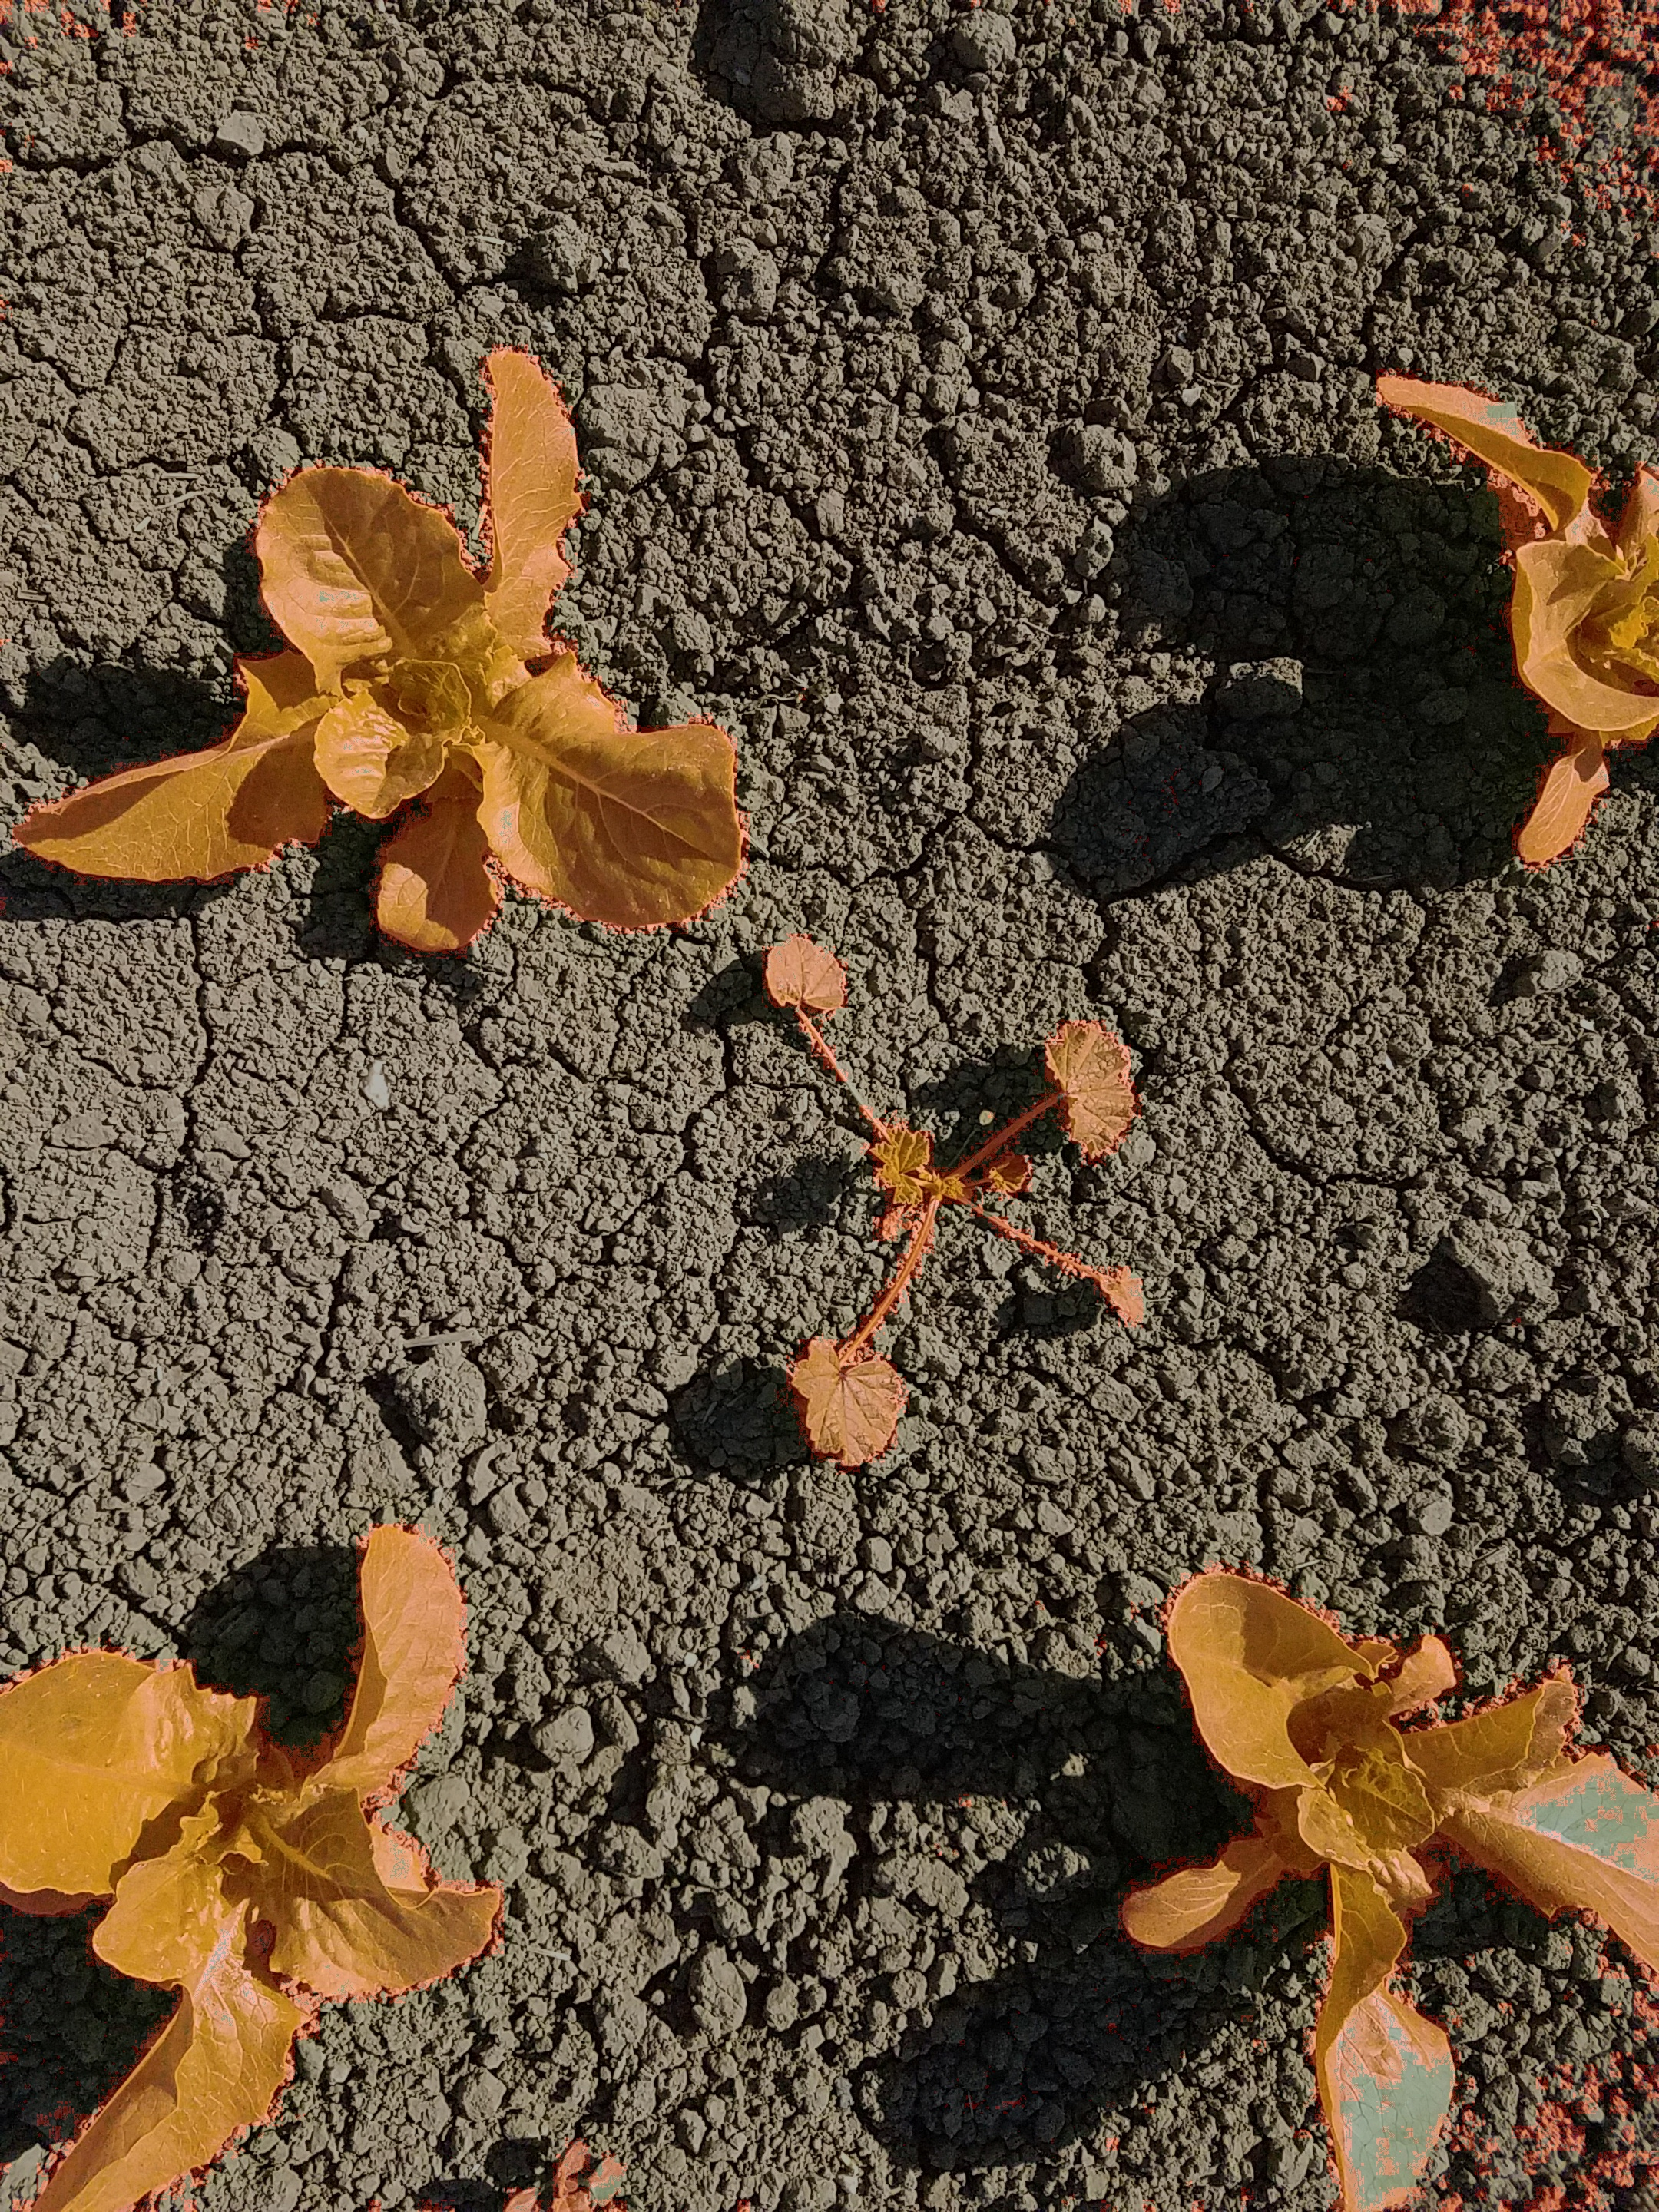
\includegraphics[width=.8\textwidth]{figures/overlay-cive.jpg}
	  \caption{CIVE mask overlay}
	  \label{fig:overlay-cive}
	\end{subfigure}
	\begin{subfigure}[t]{.40\textwidth}
	  \centering
	  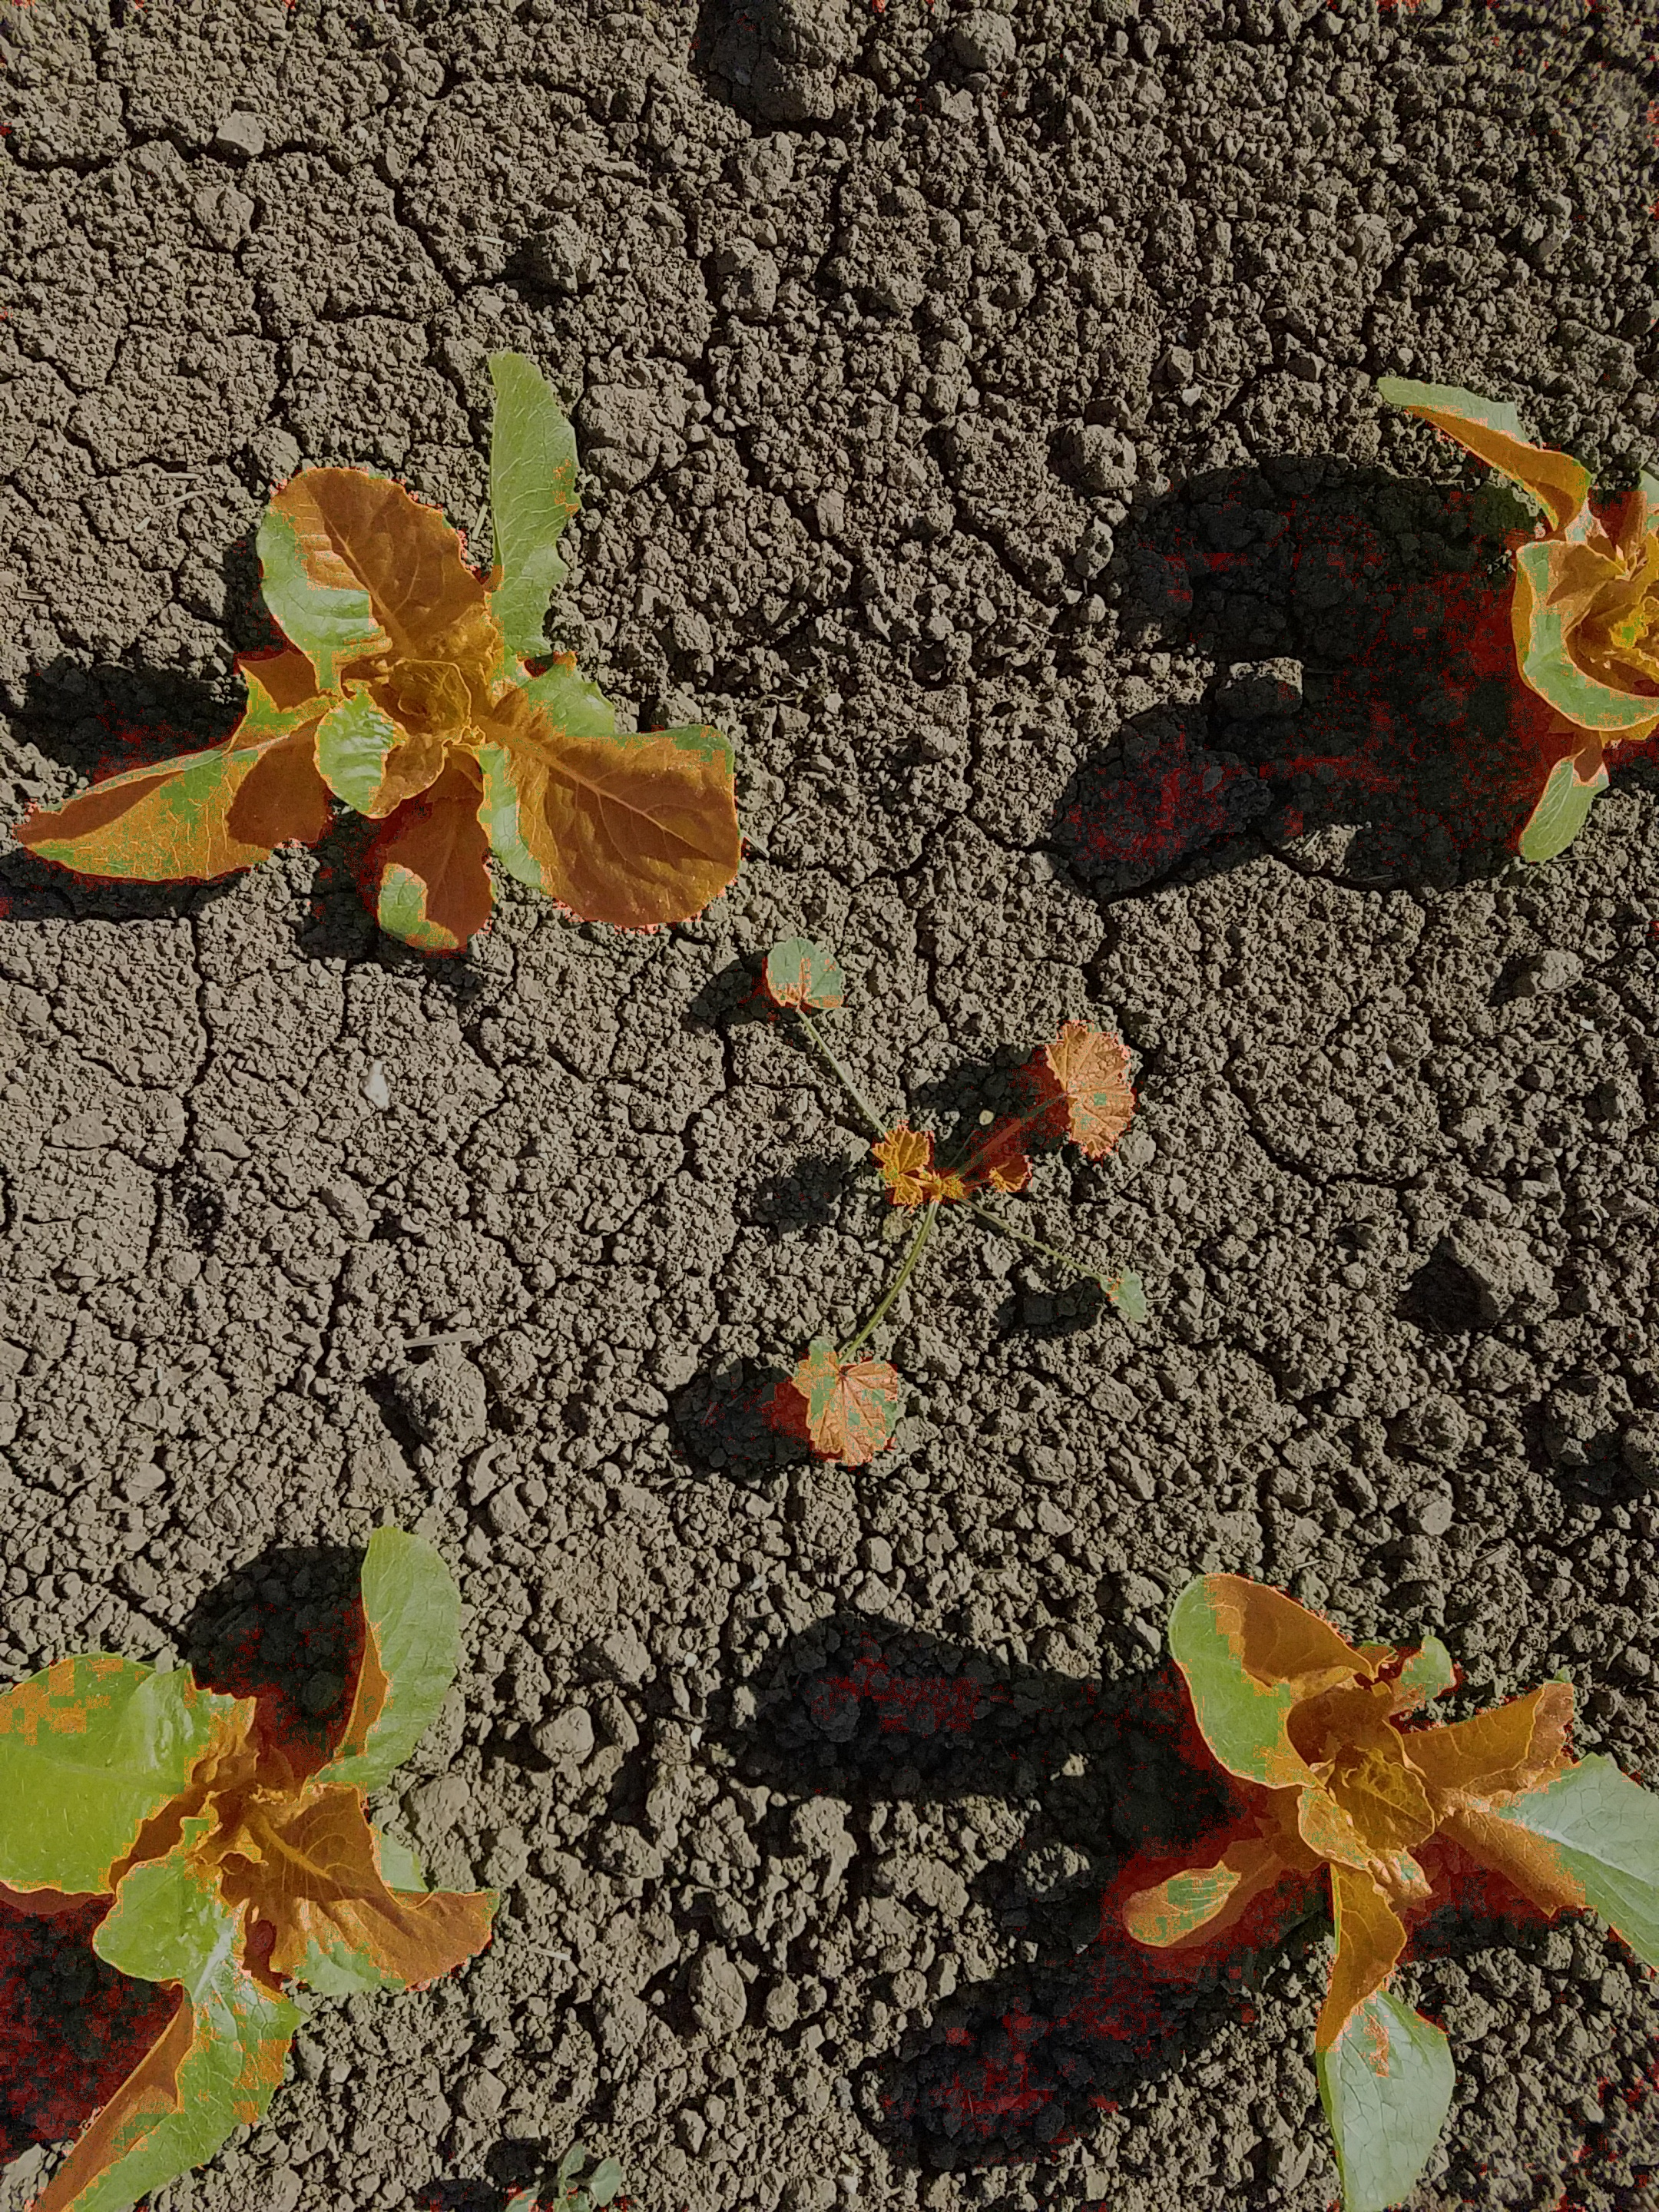
\includegraphics[width=.8\textwidth]{figures/overlay-ndi.jpg}
	  \caption{NDI mask overlay}
	  \label{fig:overlay-ndi}
	\end{subfigure}

	\caption[Masks overlayed on original images]{Masks produced with CIVE and NDI overlayed on the original image. In these images, the masks used are colored red and blended with the original image. Areas that are tinted red will be shown, so a `correct' mask will completely cover vegetation. Note the mask shown in \ref{fig:overlay-ndi} does not cover the plant completely, and segments out shadow portions of the image. What seems to be going on here is that sunlight is shining through the leaf, making the ground green enoough to be interpreted as vegetation. Contrast this with the errors seen in \ref{fig:overlay-cive}, where portions of the ground are incorrectly segmented as vegetation in cases not attributable to color contamination. (The upper right-hand portion of \ref{fig:overlay-cive} is a good example of this error.) Photo: Dr. Mark Seimens, University of Arizona.}
	\label{fig:overlay}
\end{figure}


\begin{figure}[H]
\centering
\begin{tabular}{ccc}
\subfloat[NDI]{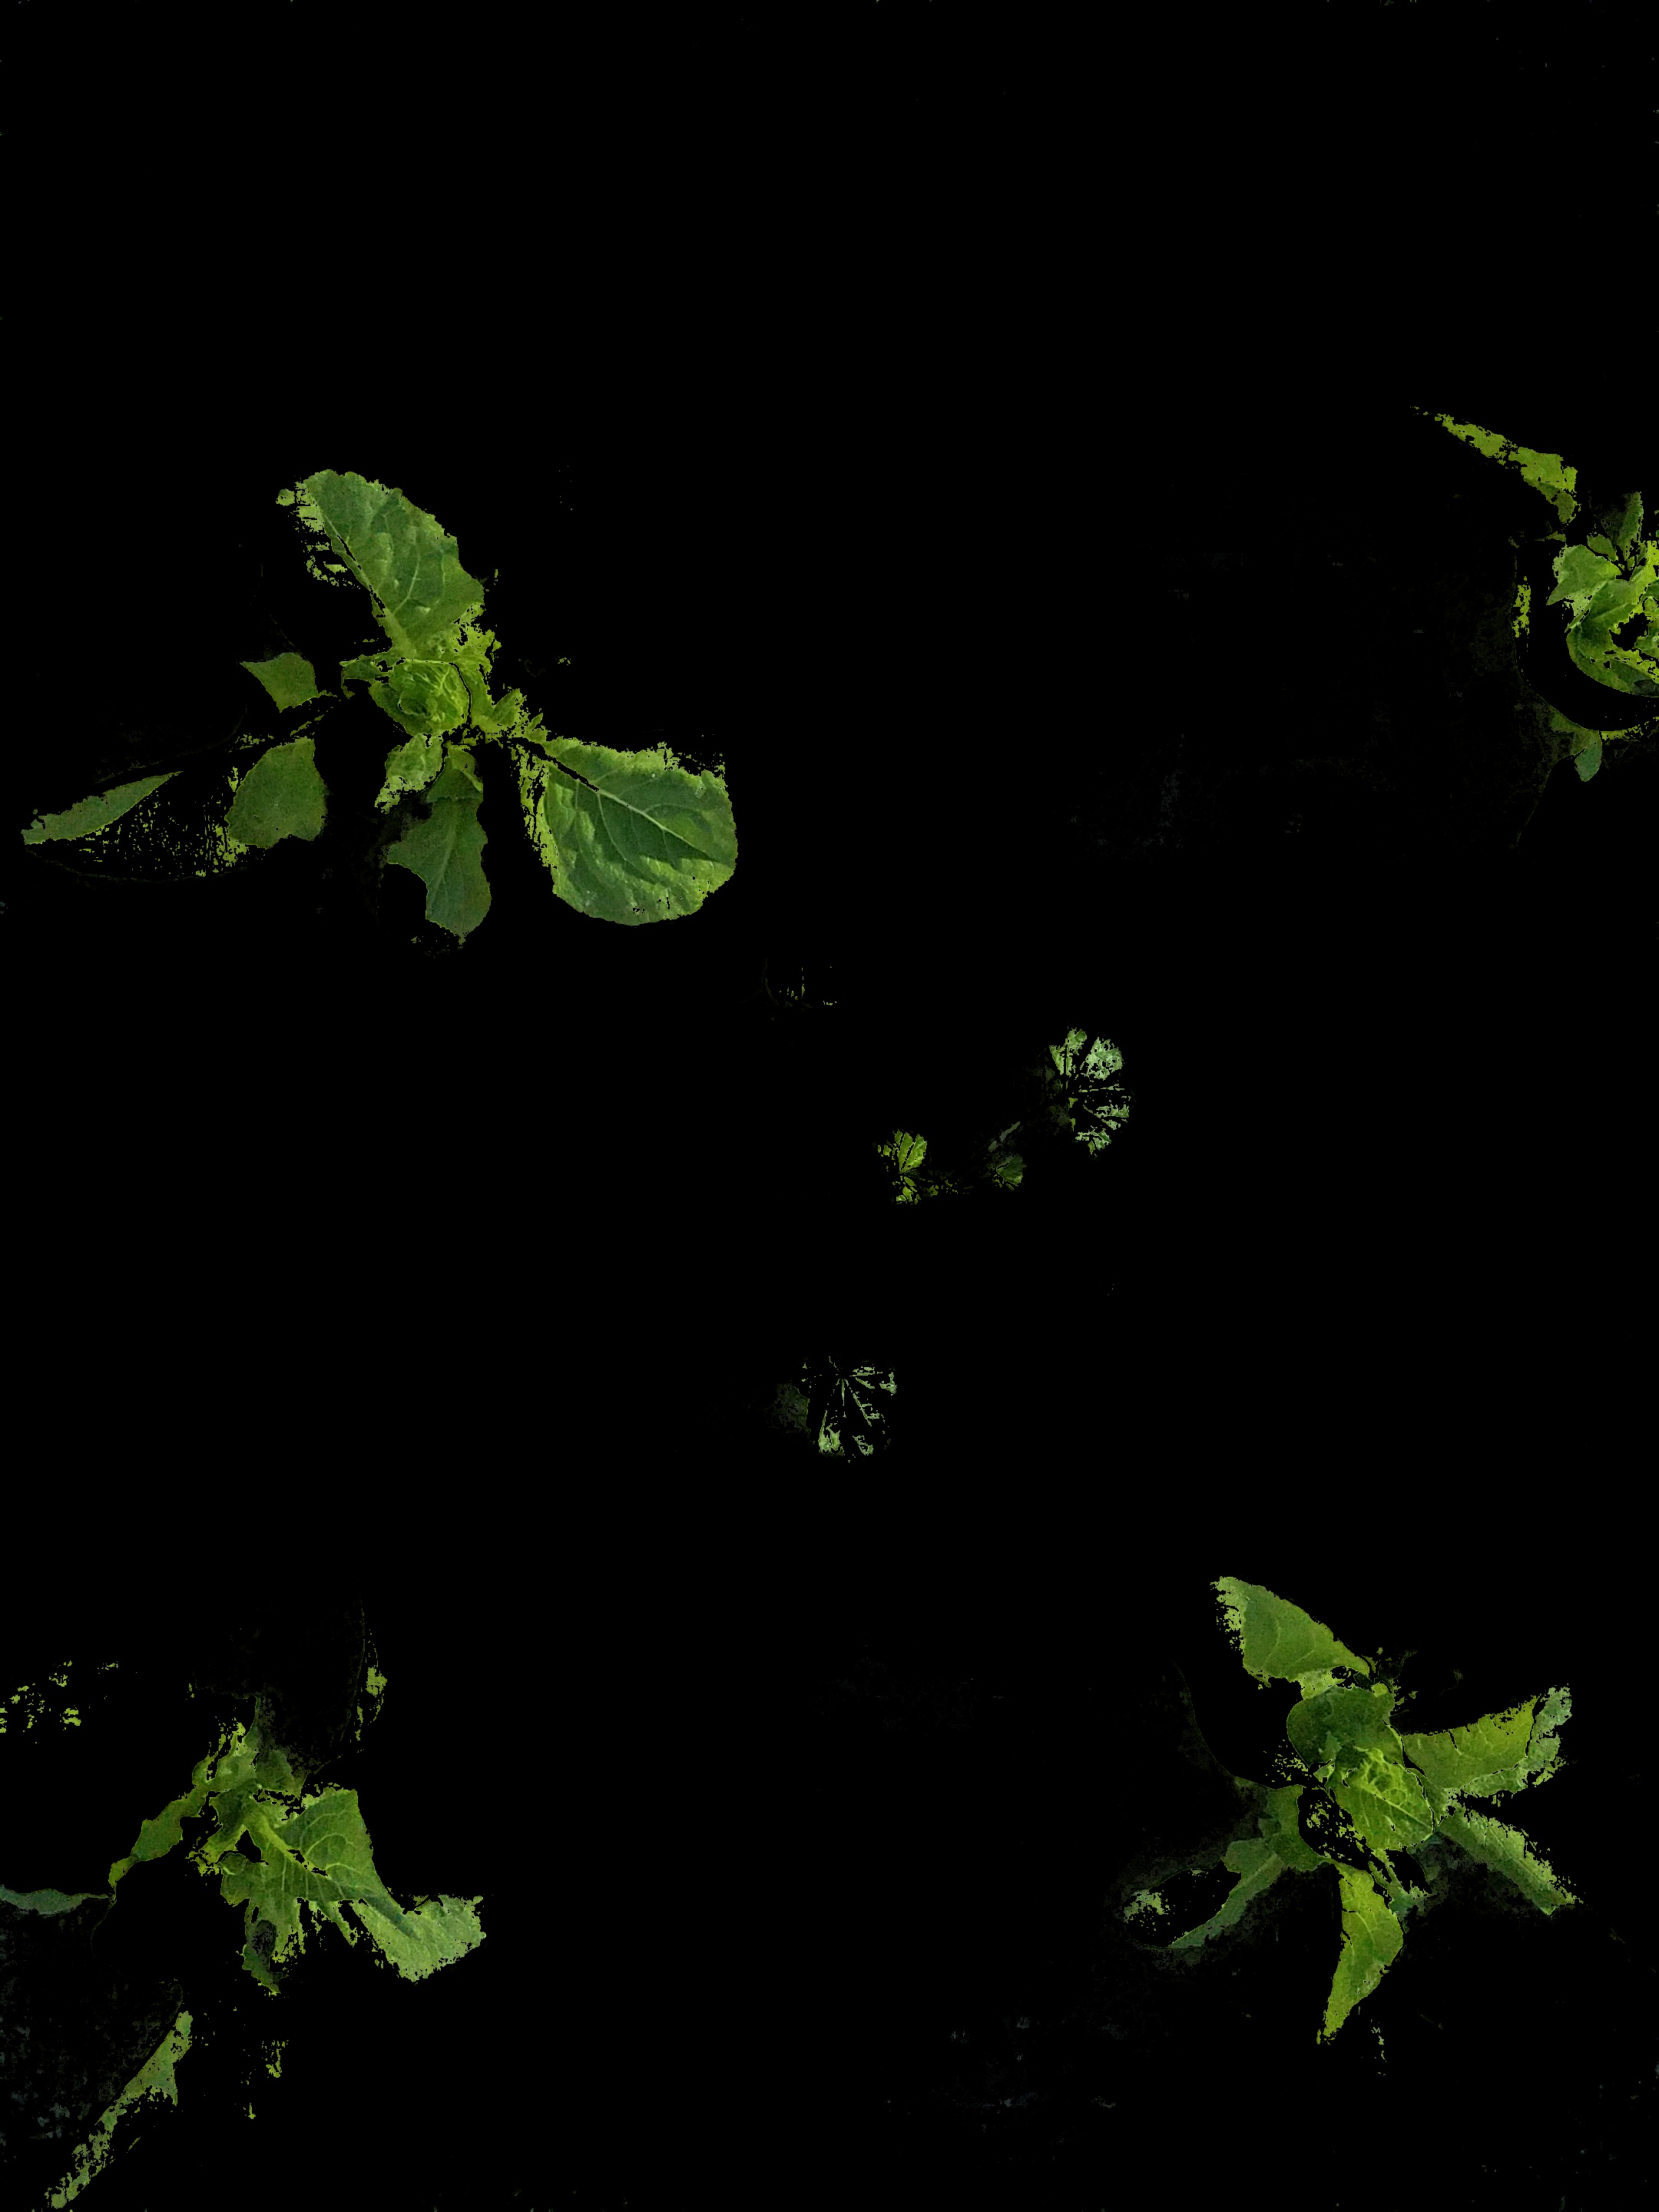
\includegraphics[width = 1.25in]{figures/20201117_112624-NDI.jpg} \label{fig:ndi}} &
\subfloat[EXG]{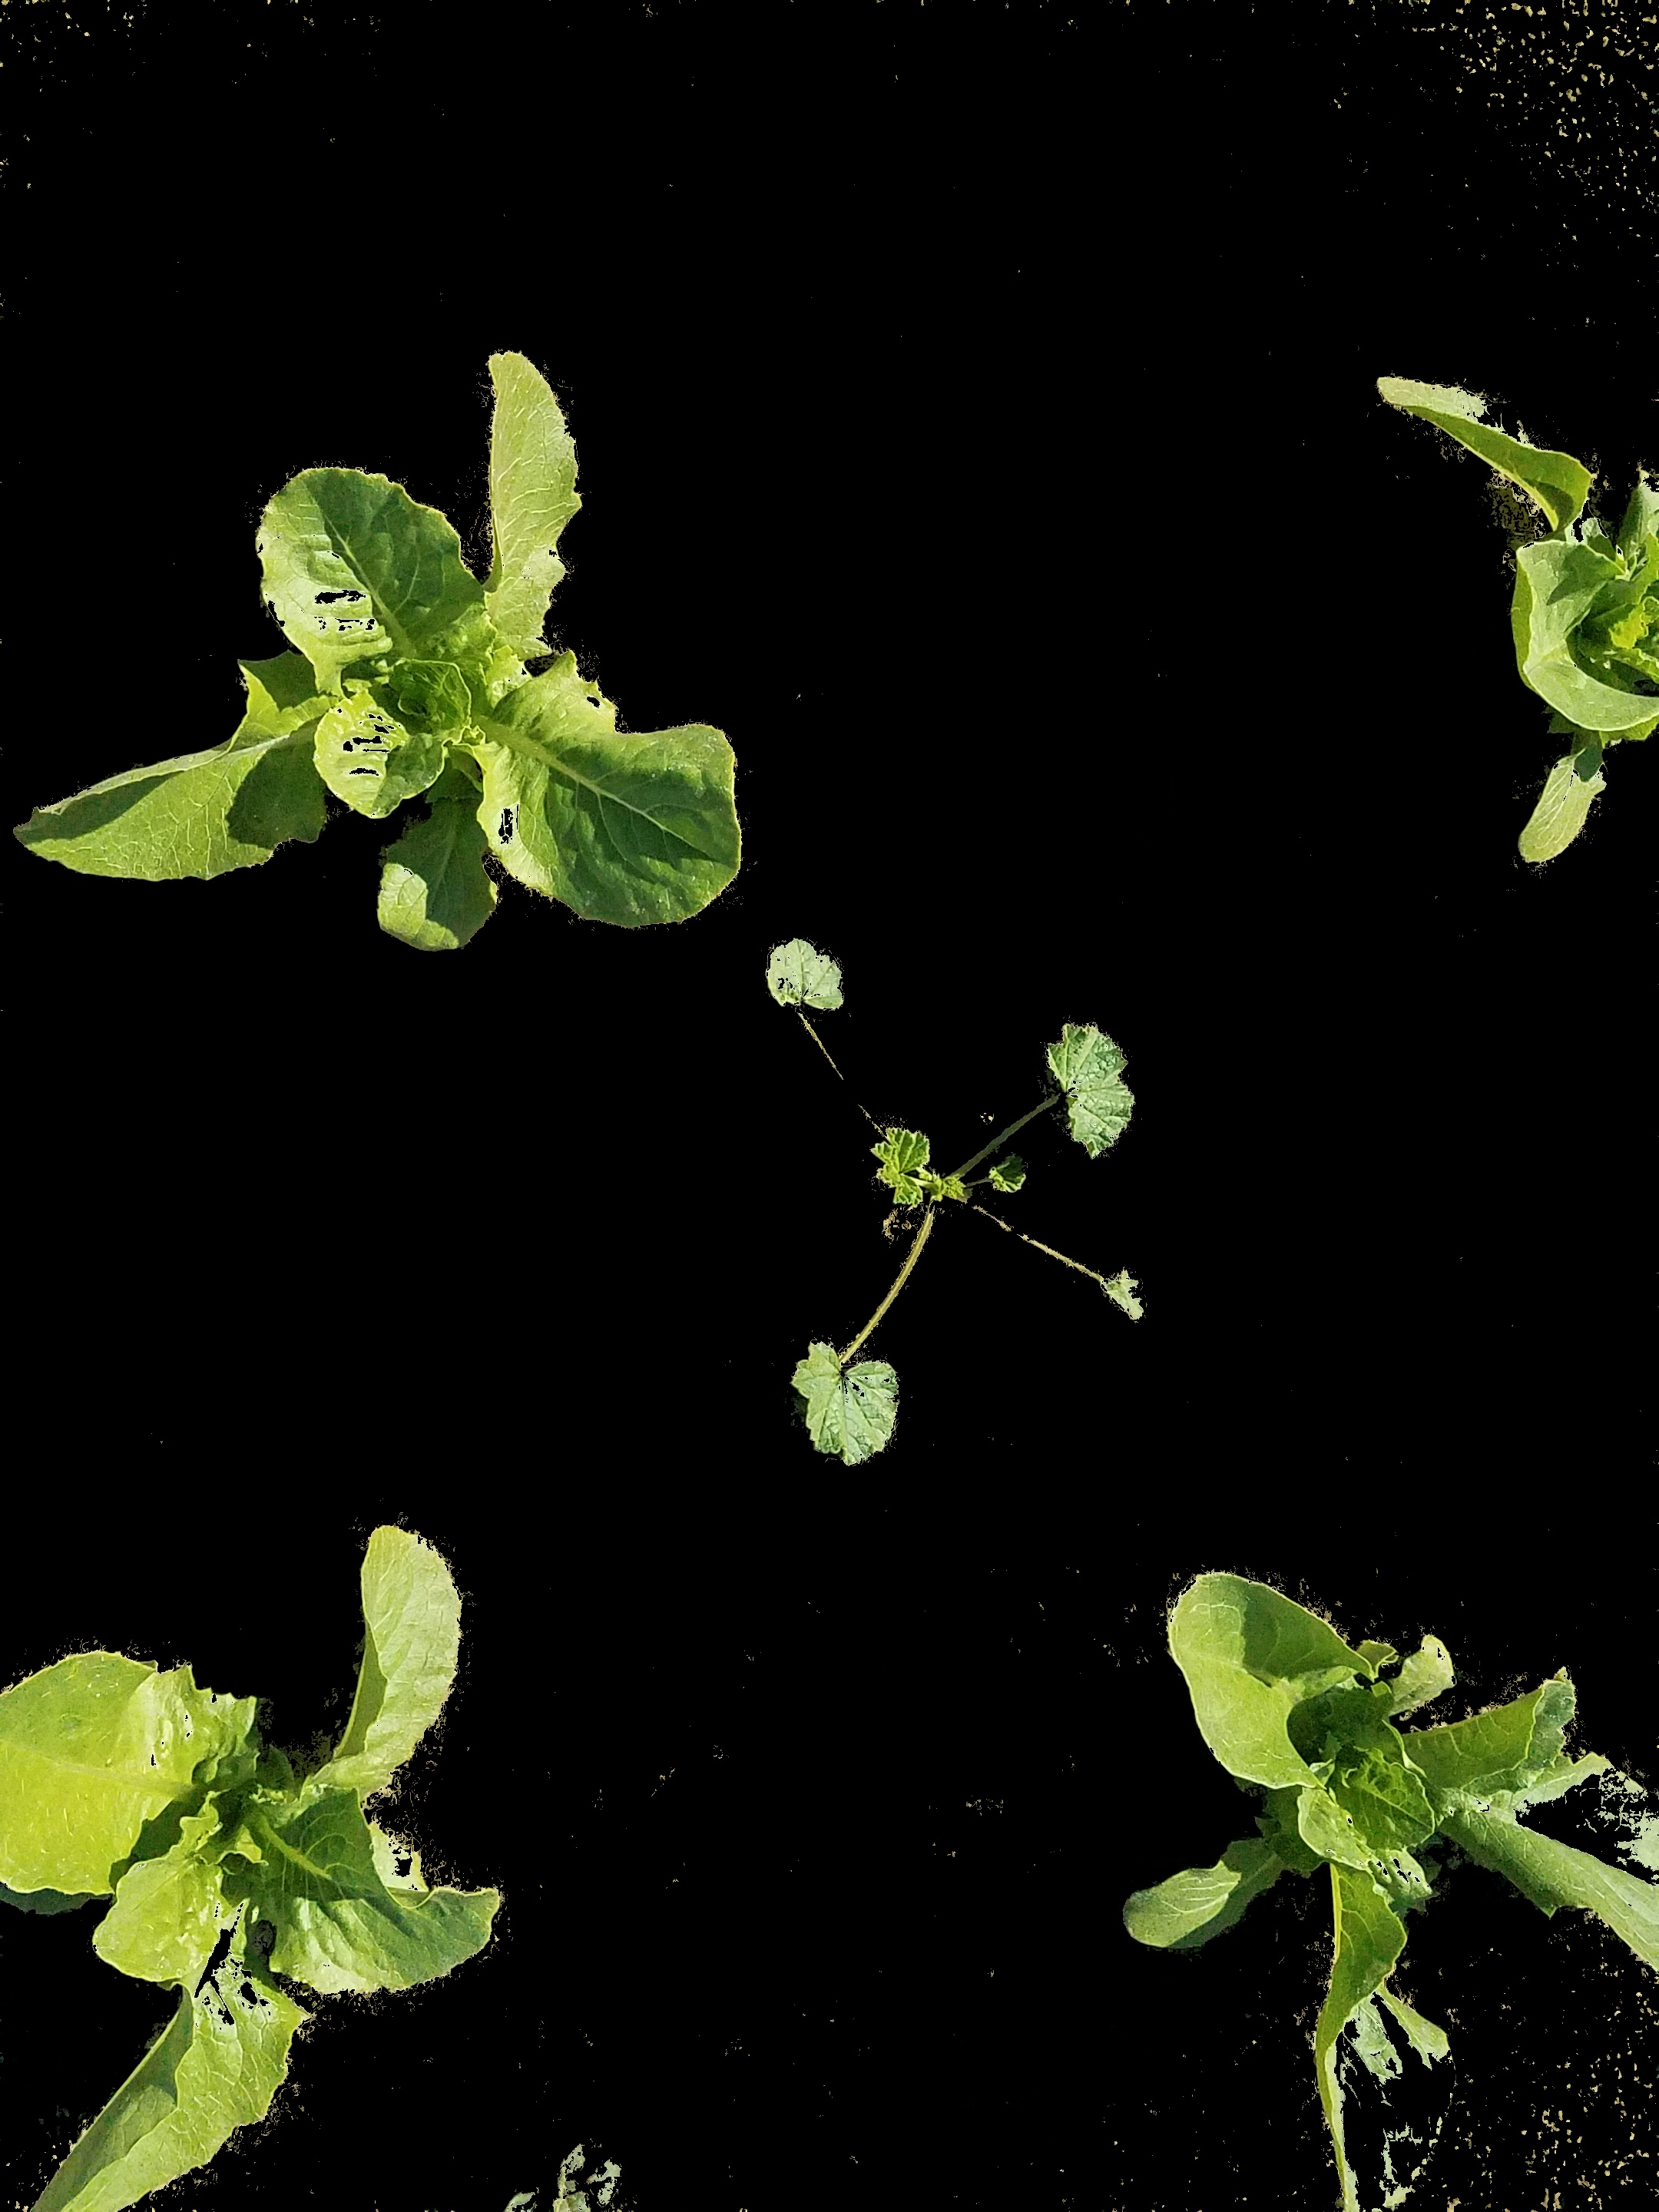
\includegraphics[width = 1.25in]{figures/20201117_112624-ExG.jpg} \label{fig:exg}} &
\subfloat[EXR]{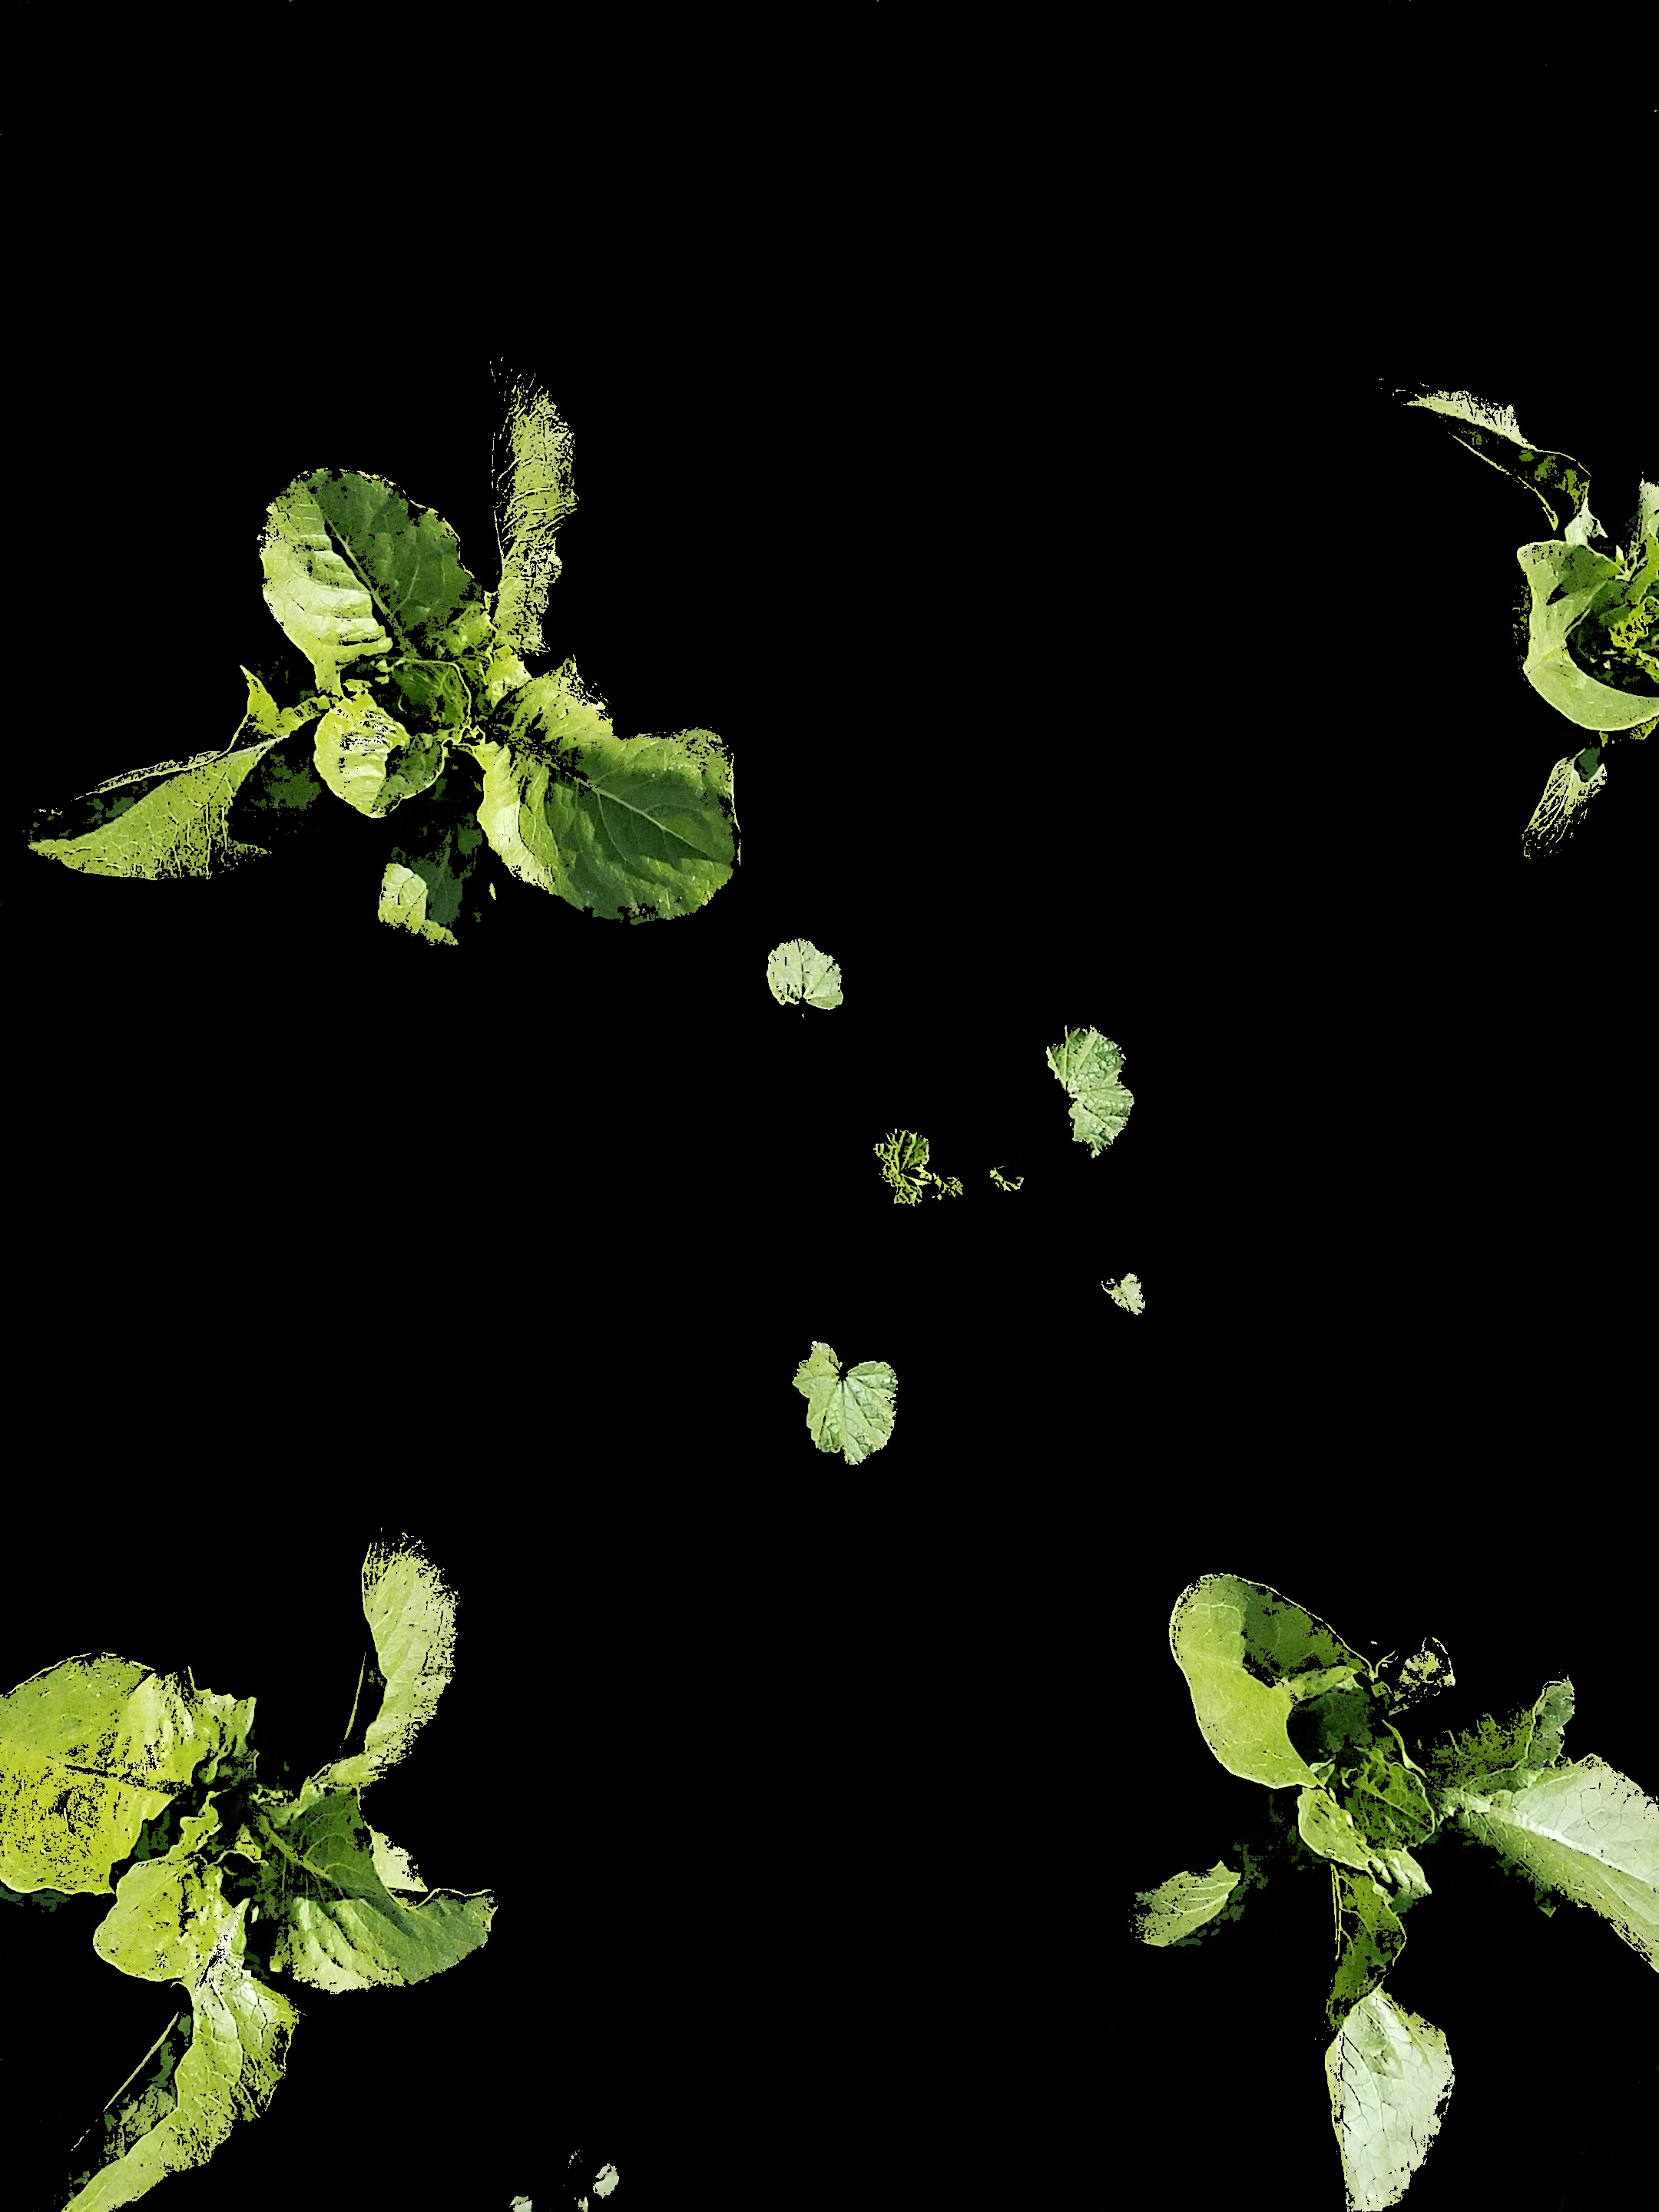
\includegraphics[width = 1.25in]{figures/20201117_112624-ExR.jpg} \label{fig:exr}} \\
\subfloat[CIVE]{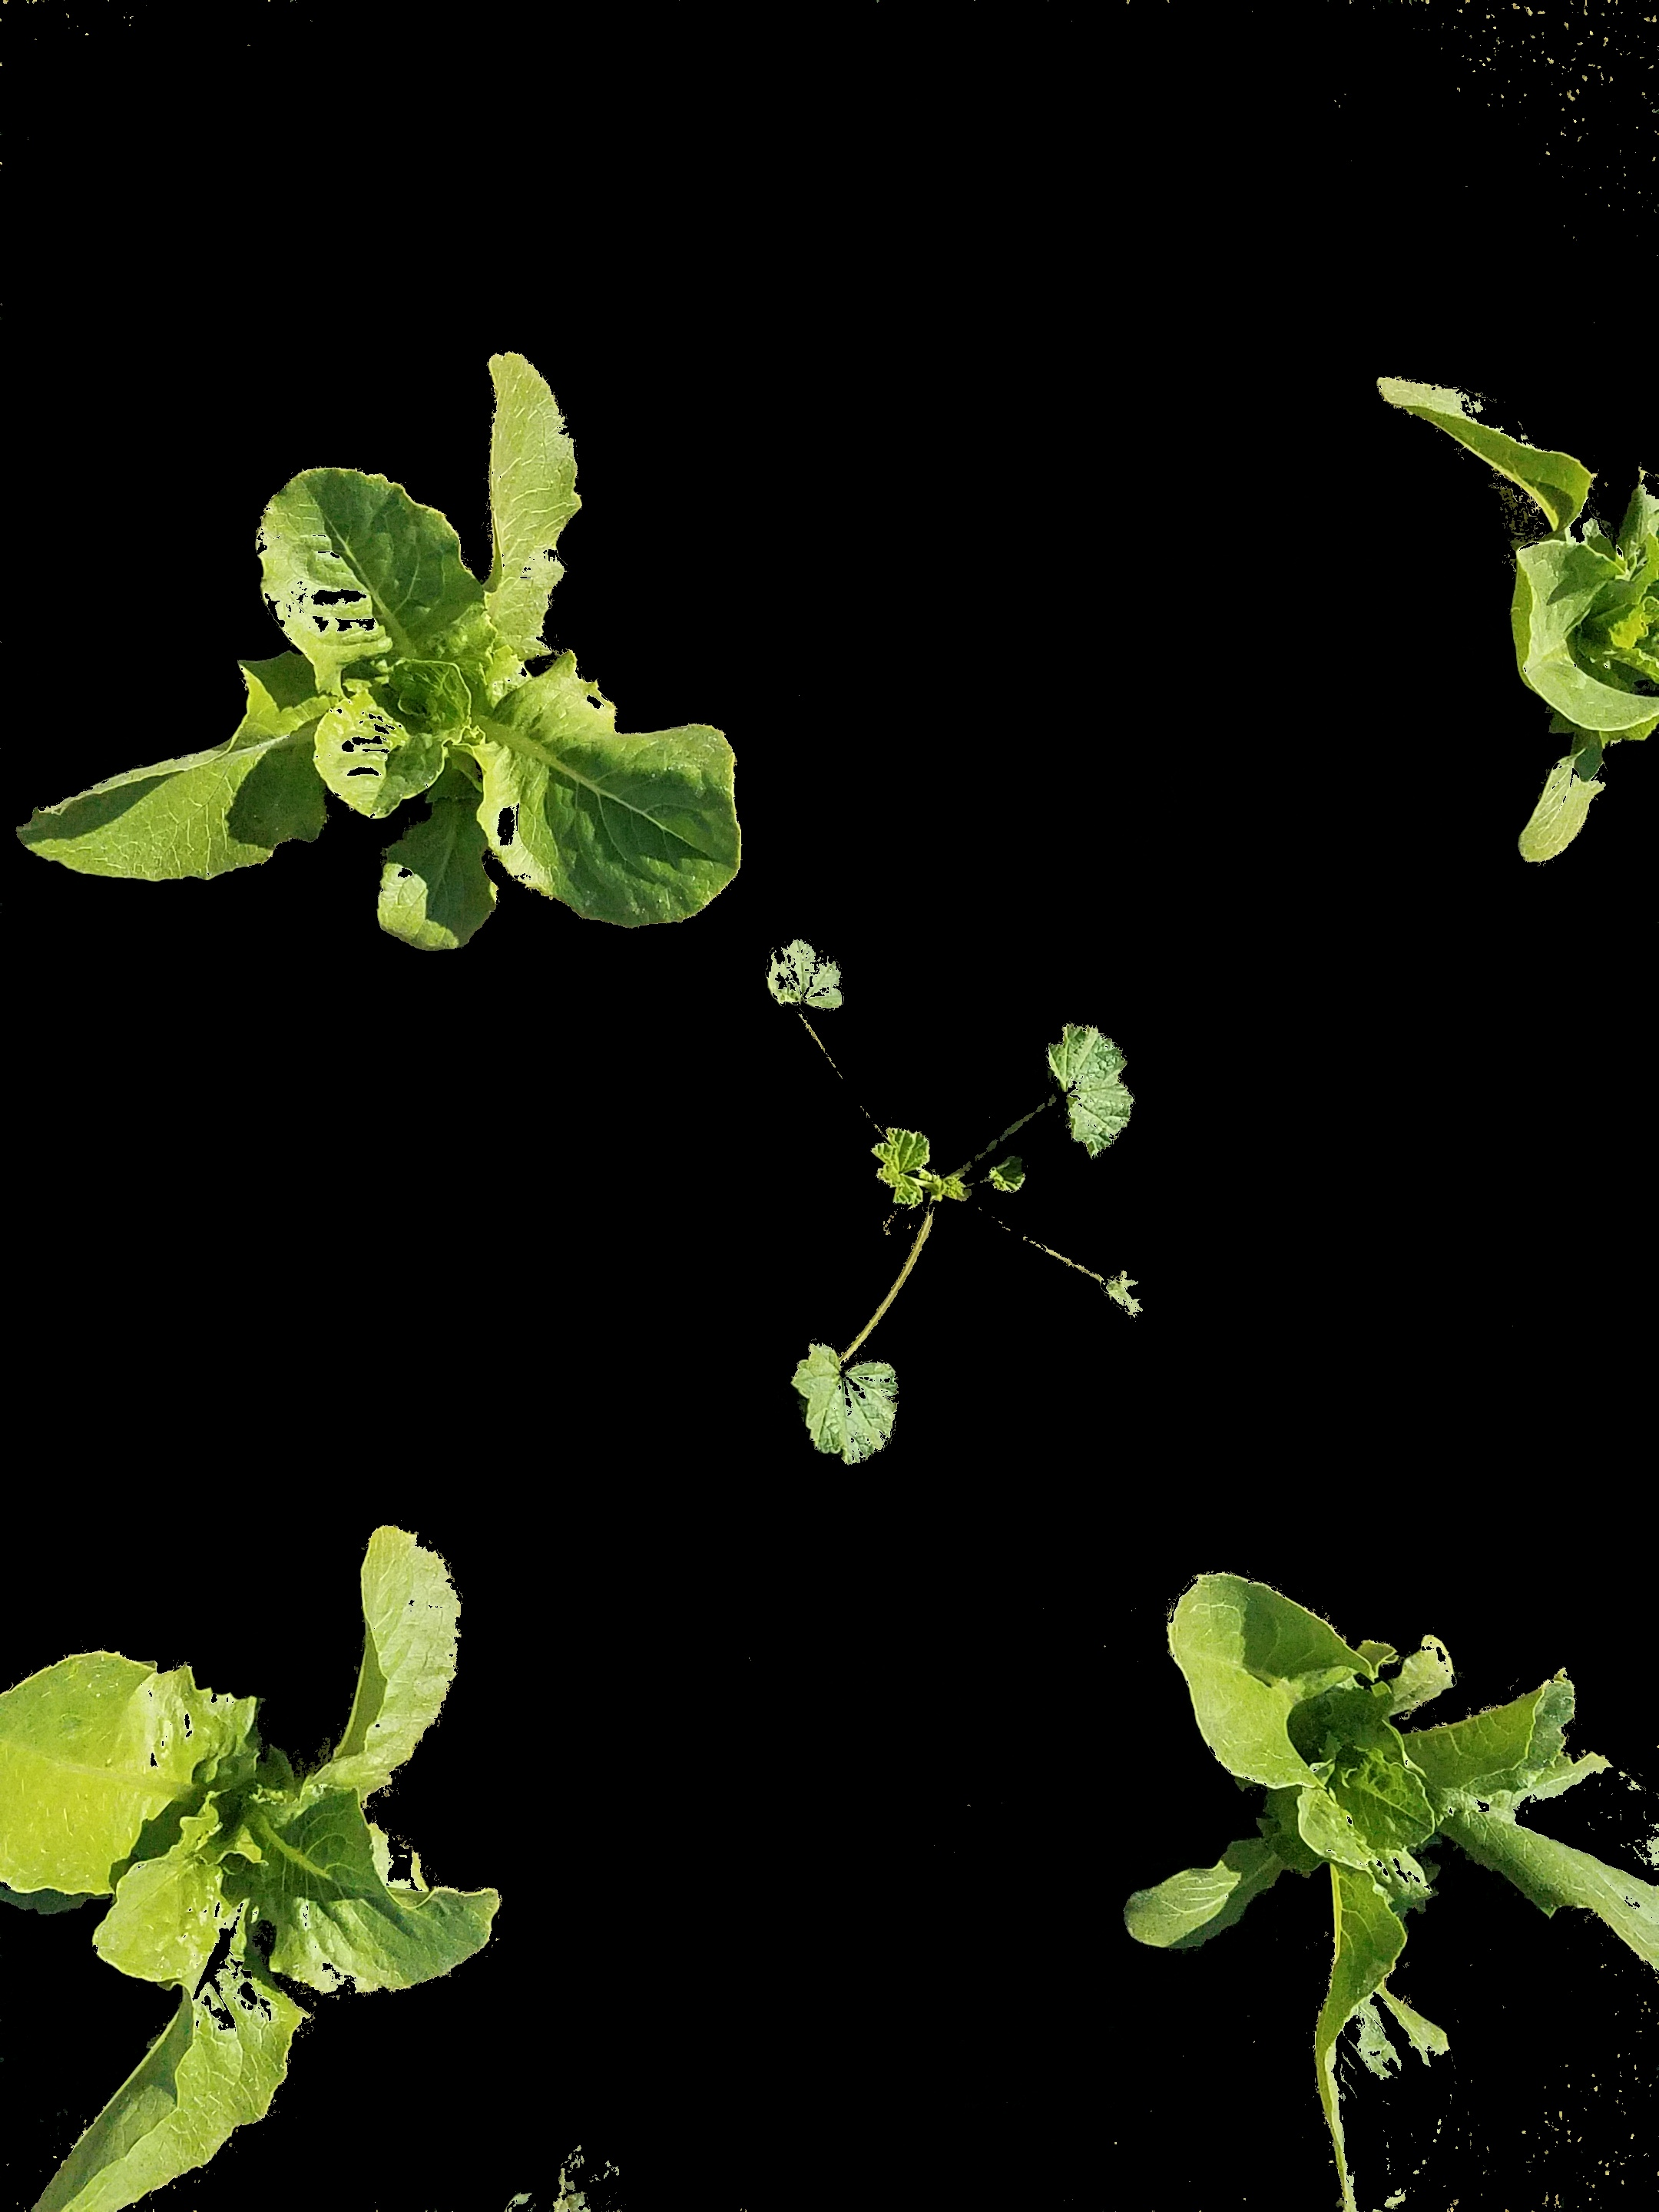
\includegraphics[width = 1.25in]{figures/20201117_112624-CIVE.jpg} \label{fig:cive}} &
\subfloat[EXG-EXR]{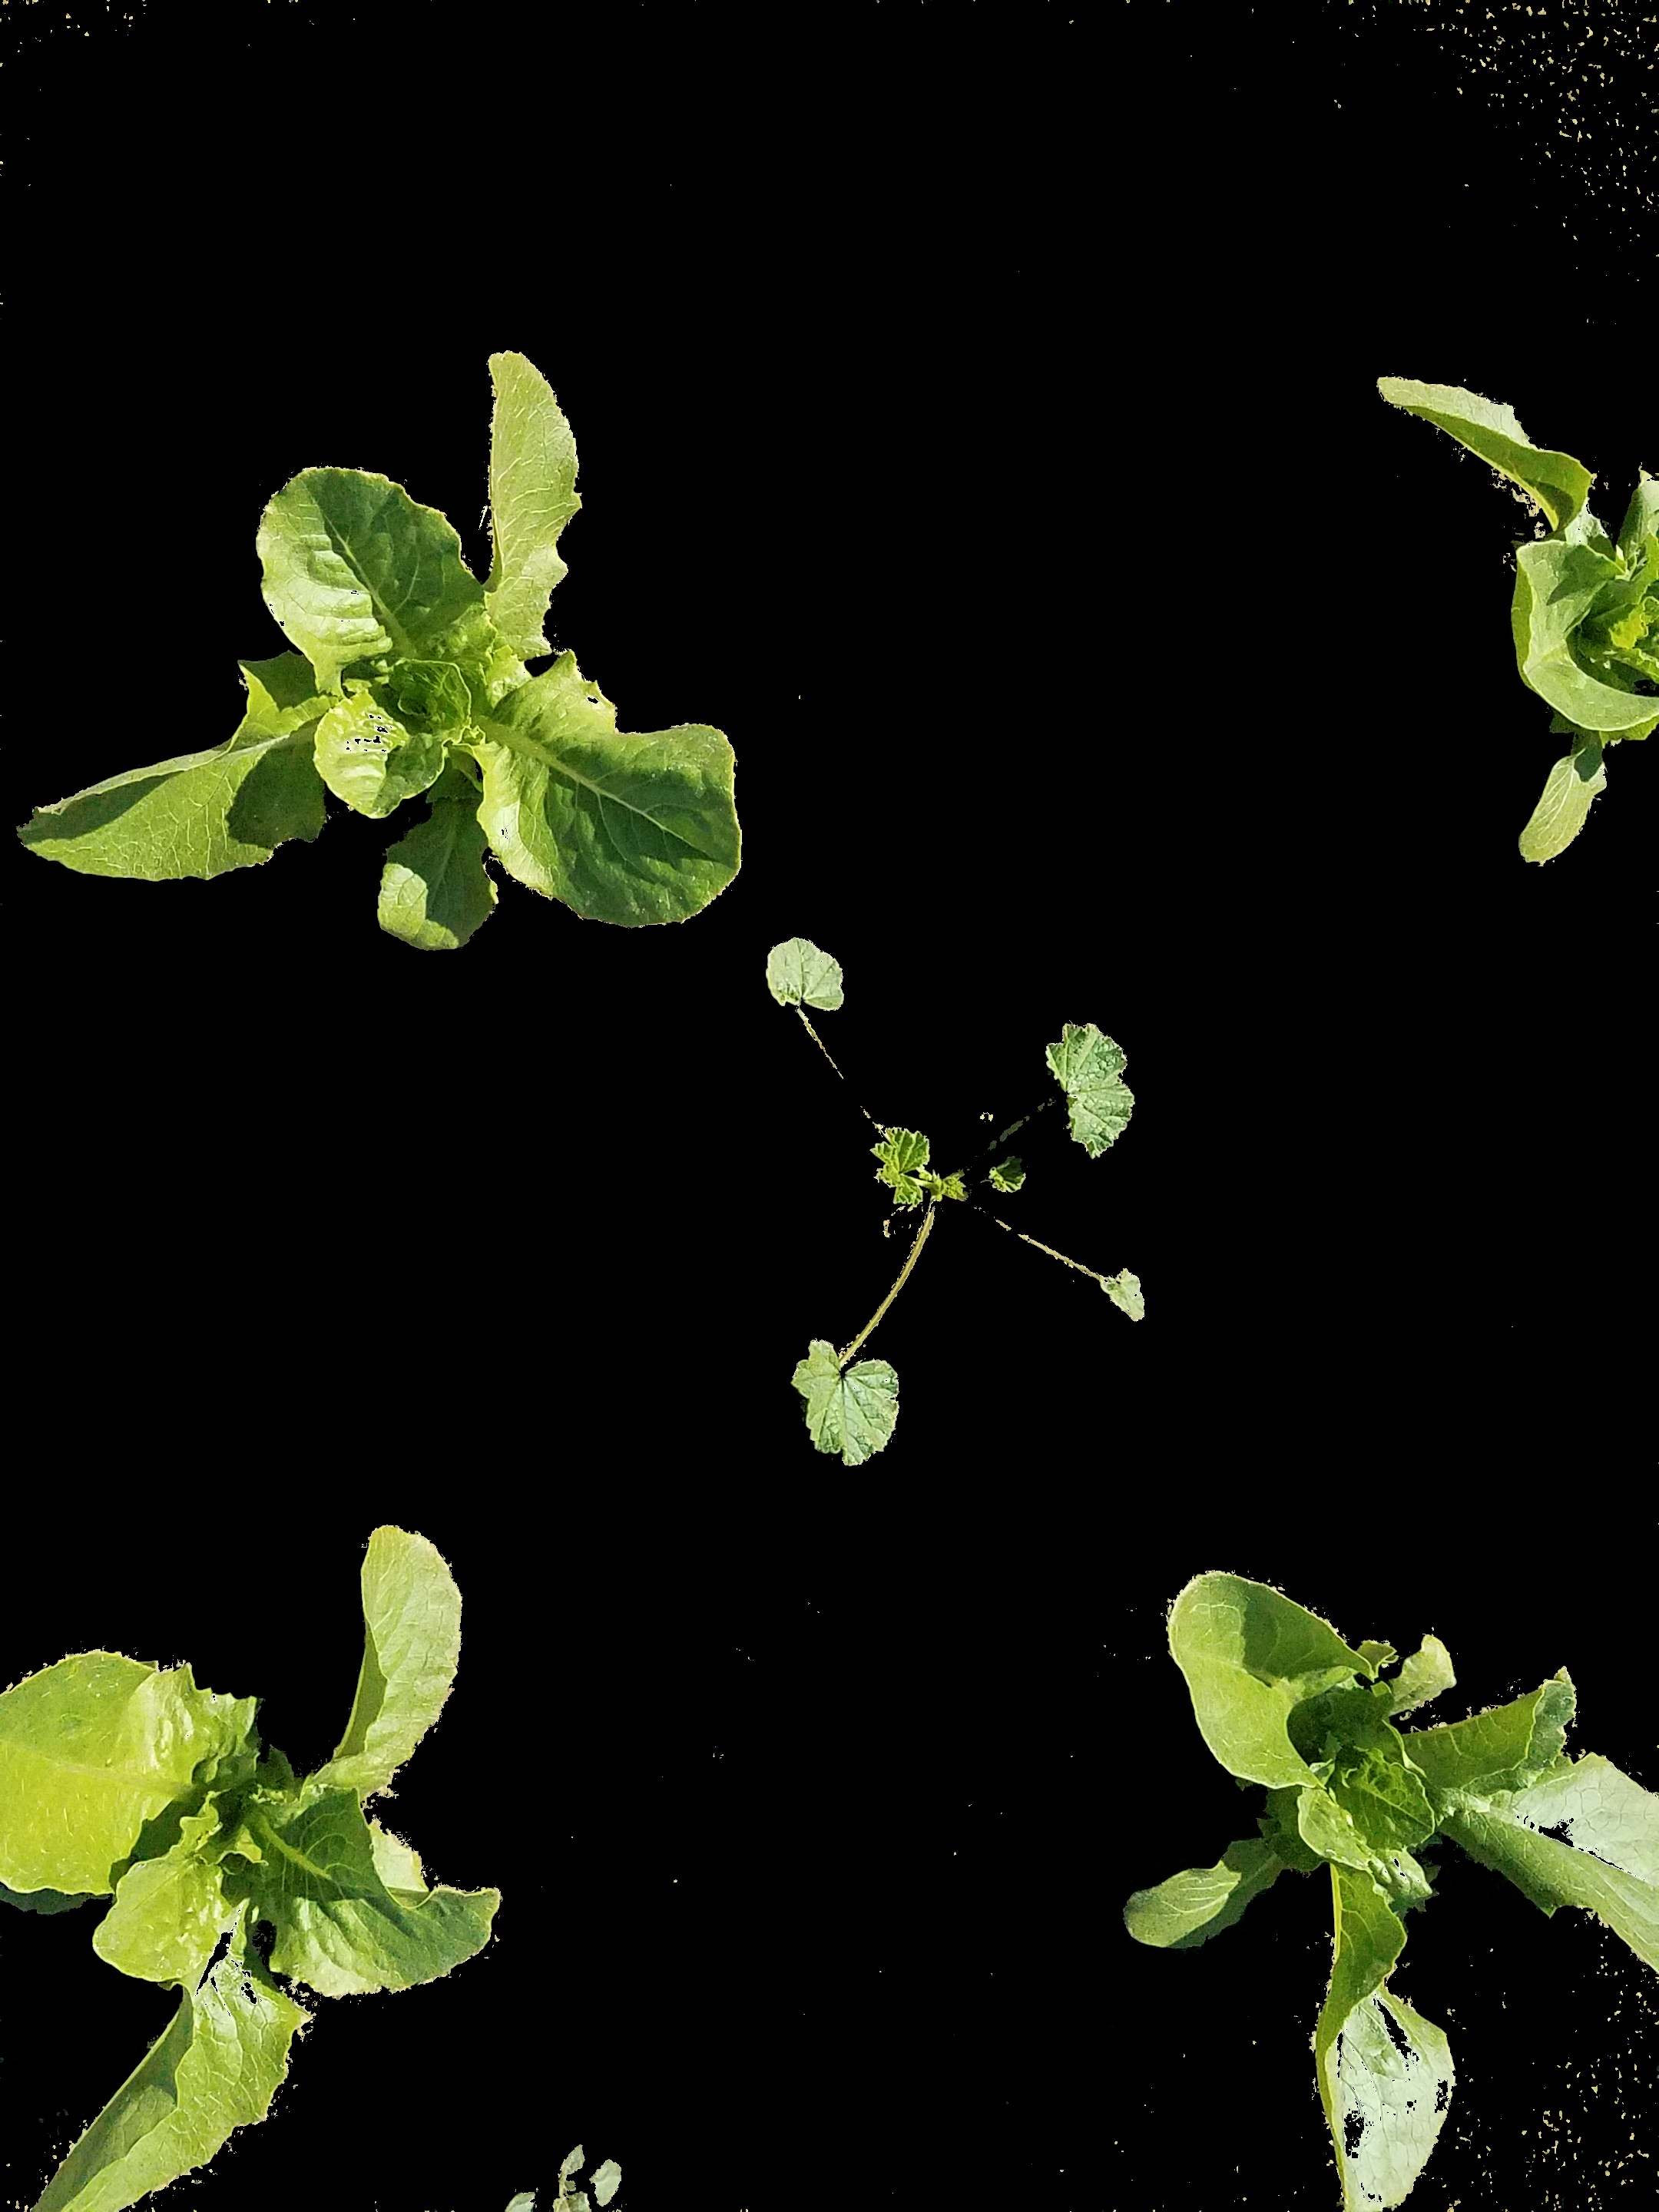
\includegraphics[width = 1.25in]{figures/20201117_112624-ExGR.jpg} \label{fig:exgexr}} &
\subfloat[NGRDI]{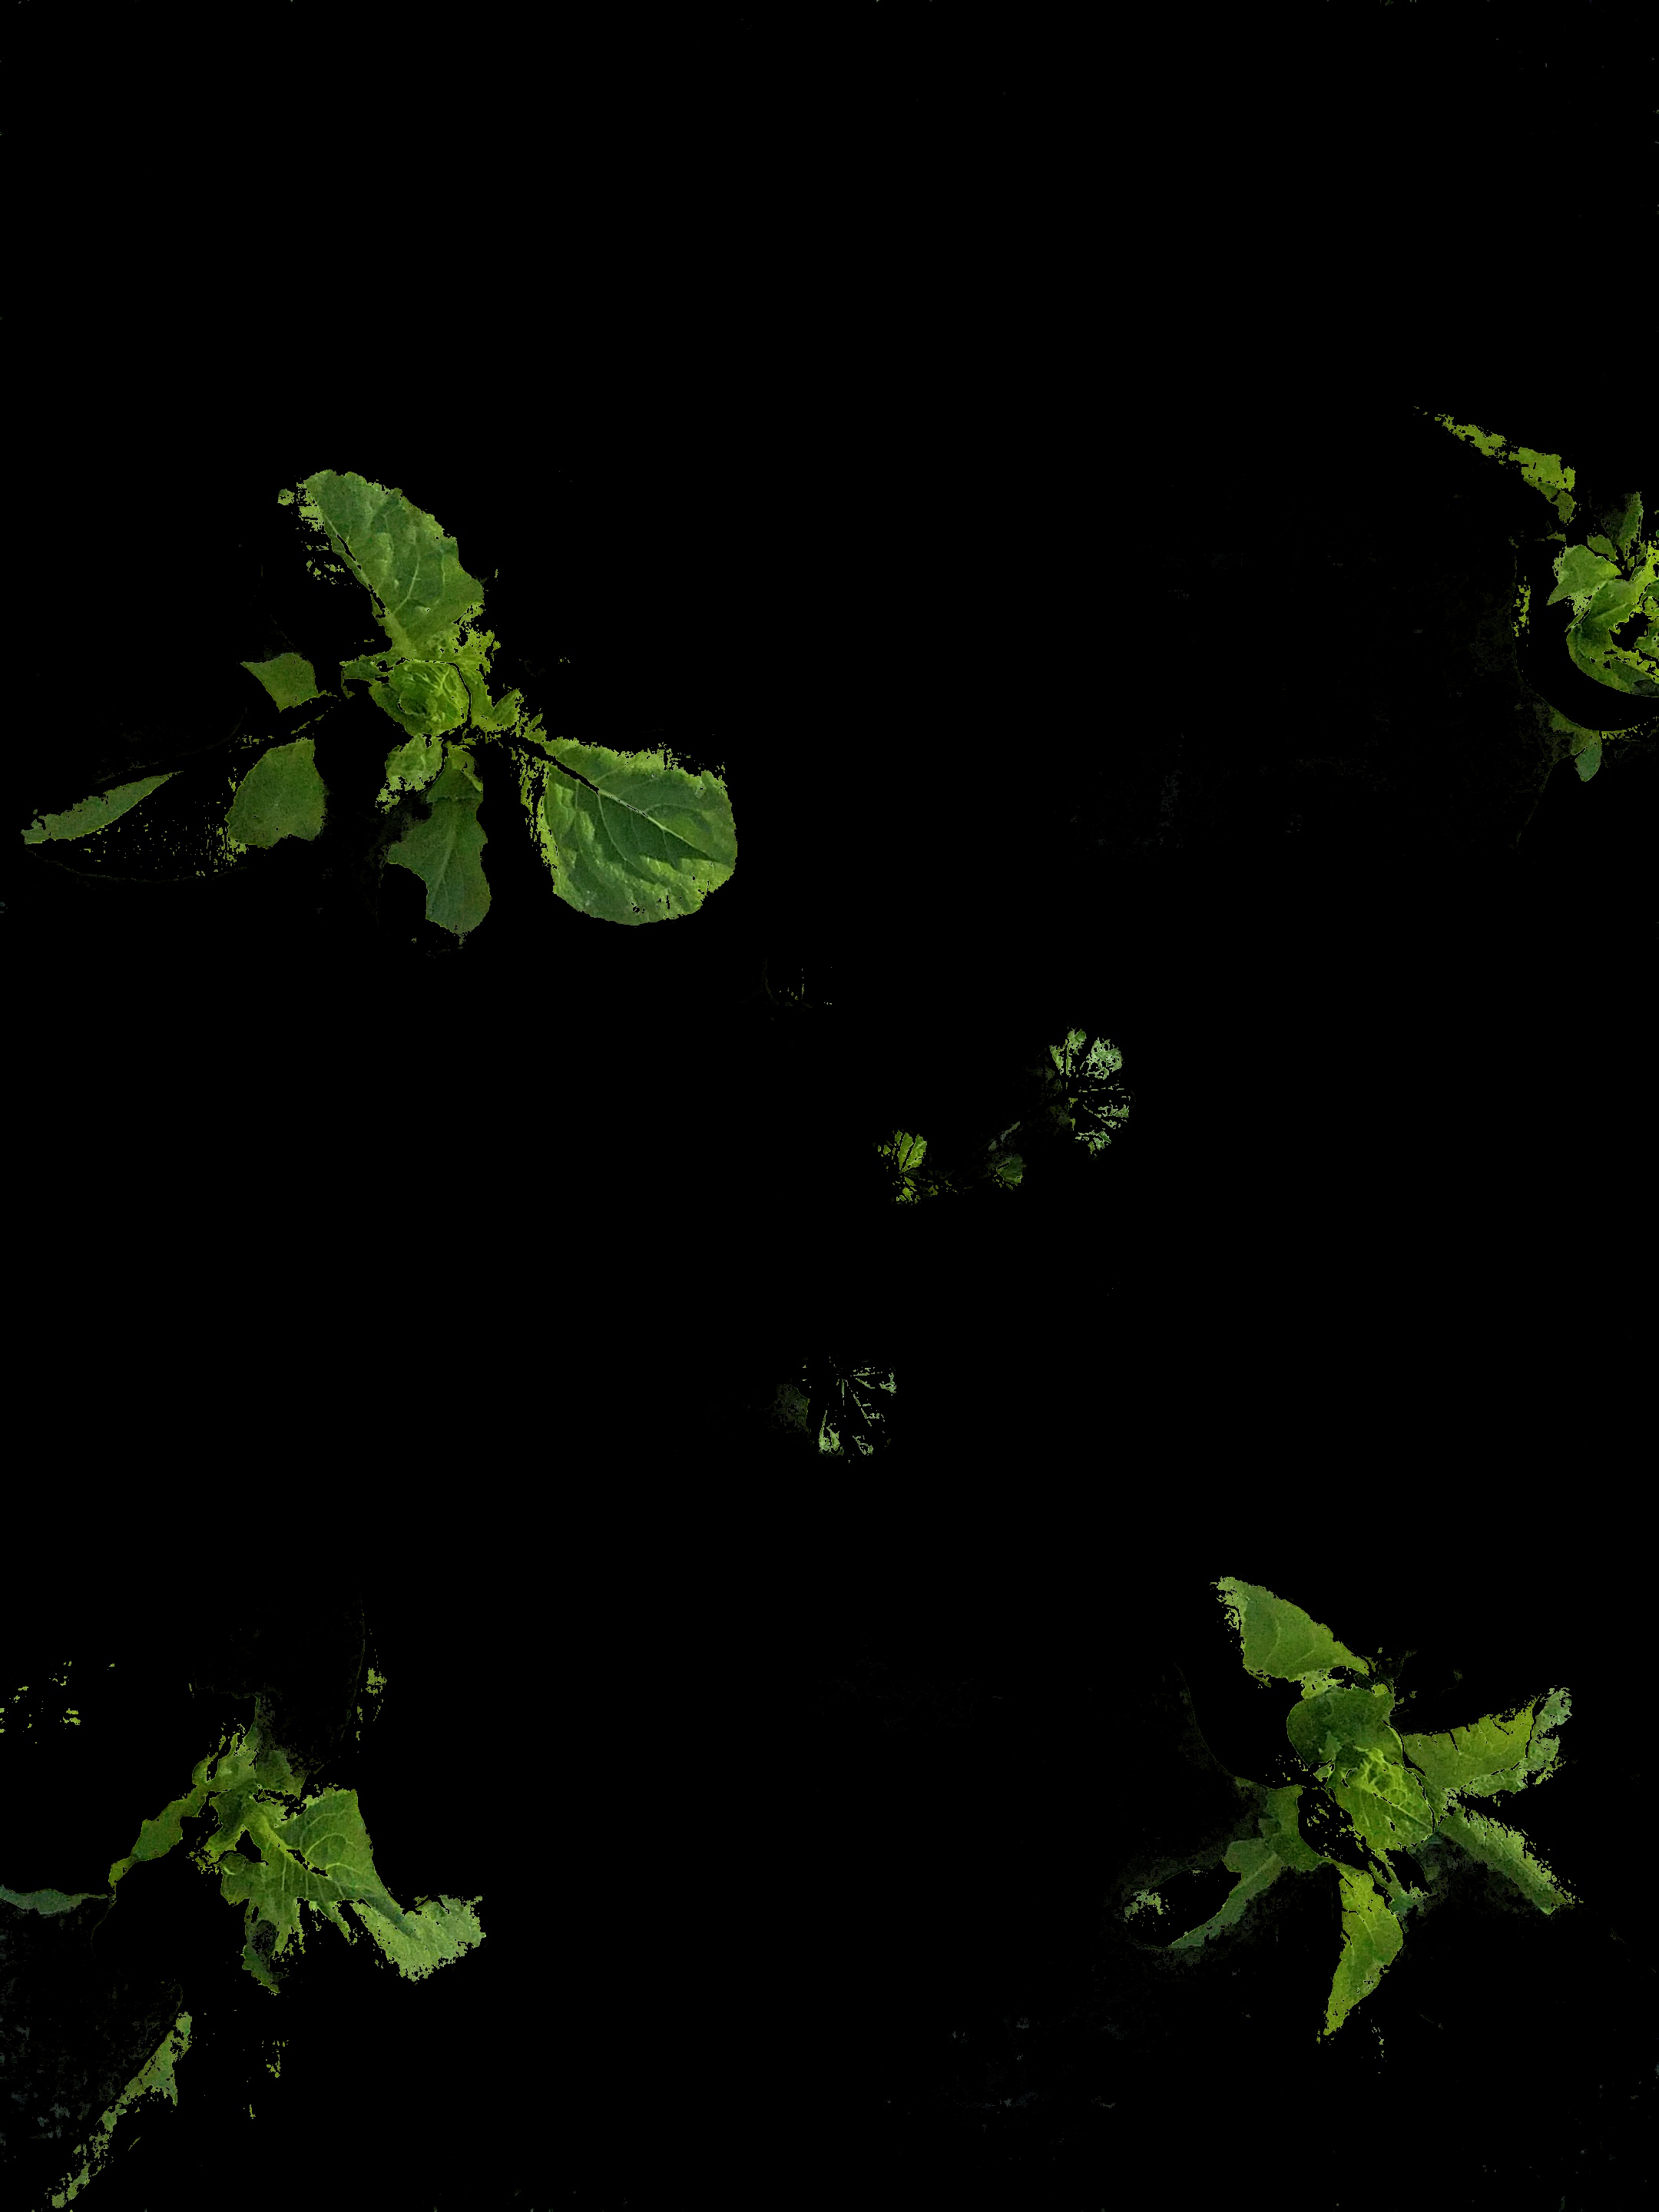
\includegraphics[width = 1.25in]{figures/20201117_112624-NGRDI.jpg} \label{fig:nrgdi}} \\
\subfloat[Com1]{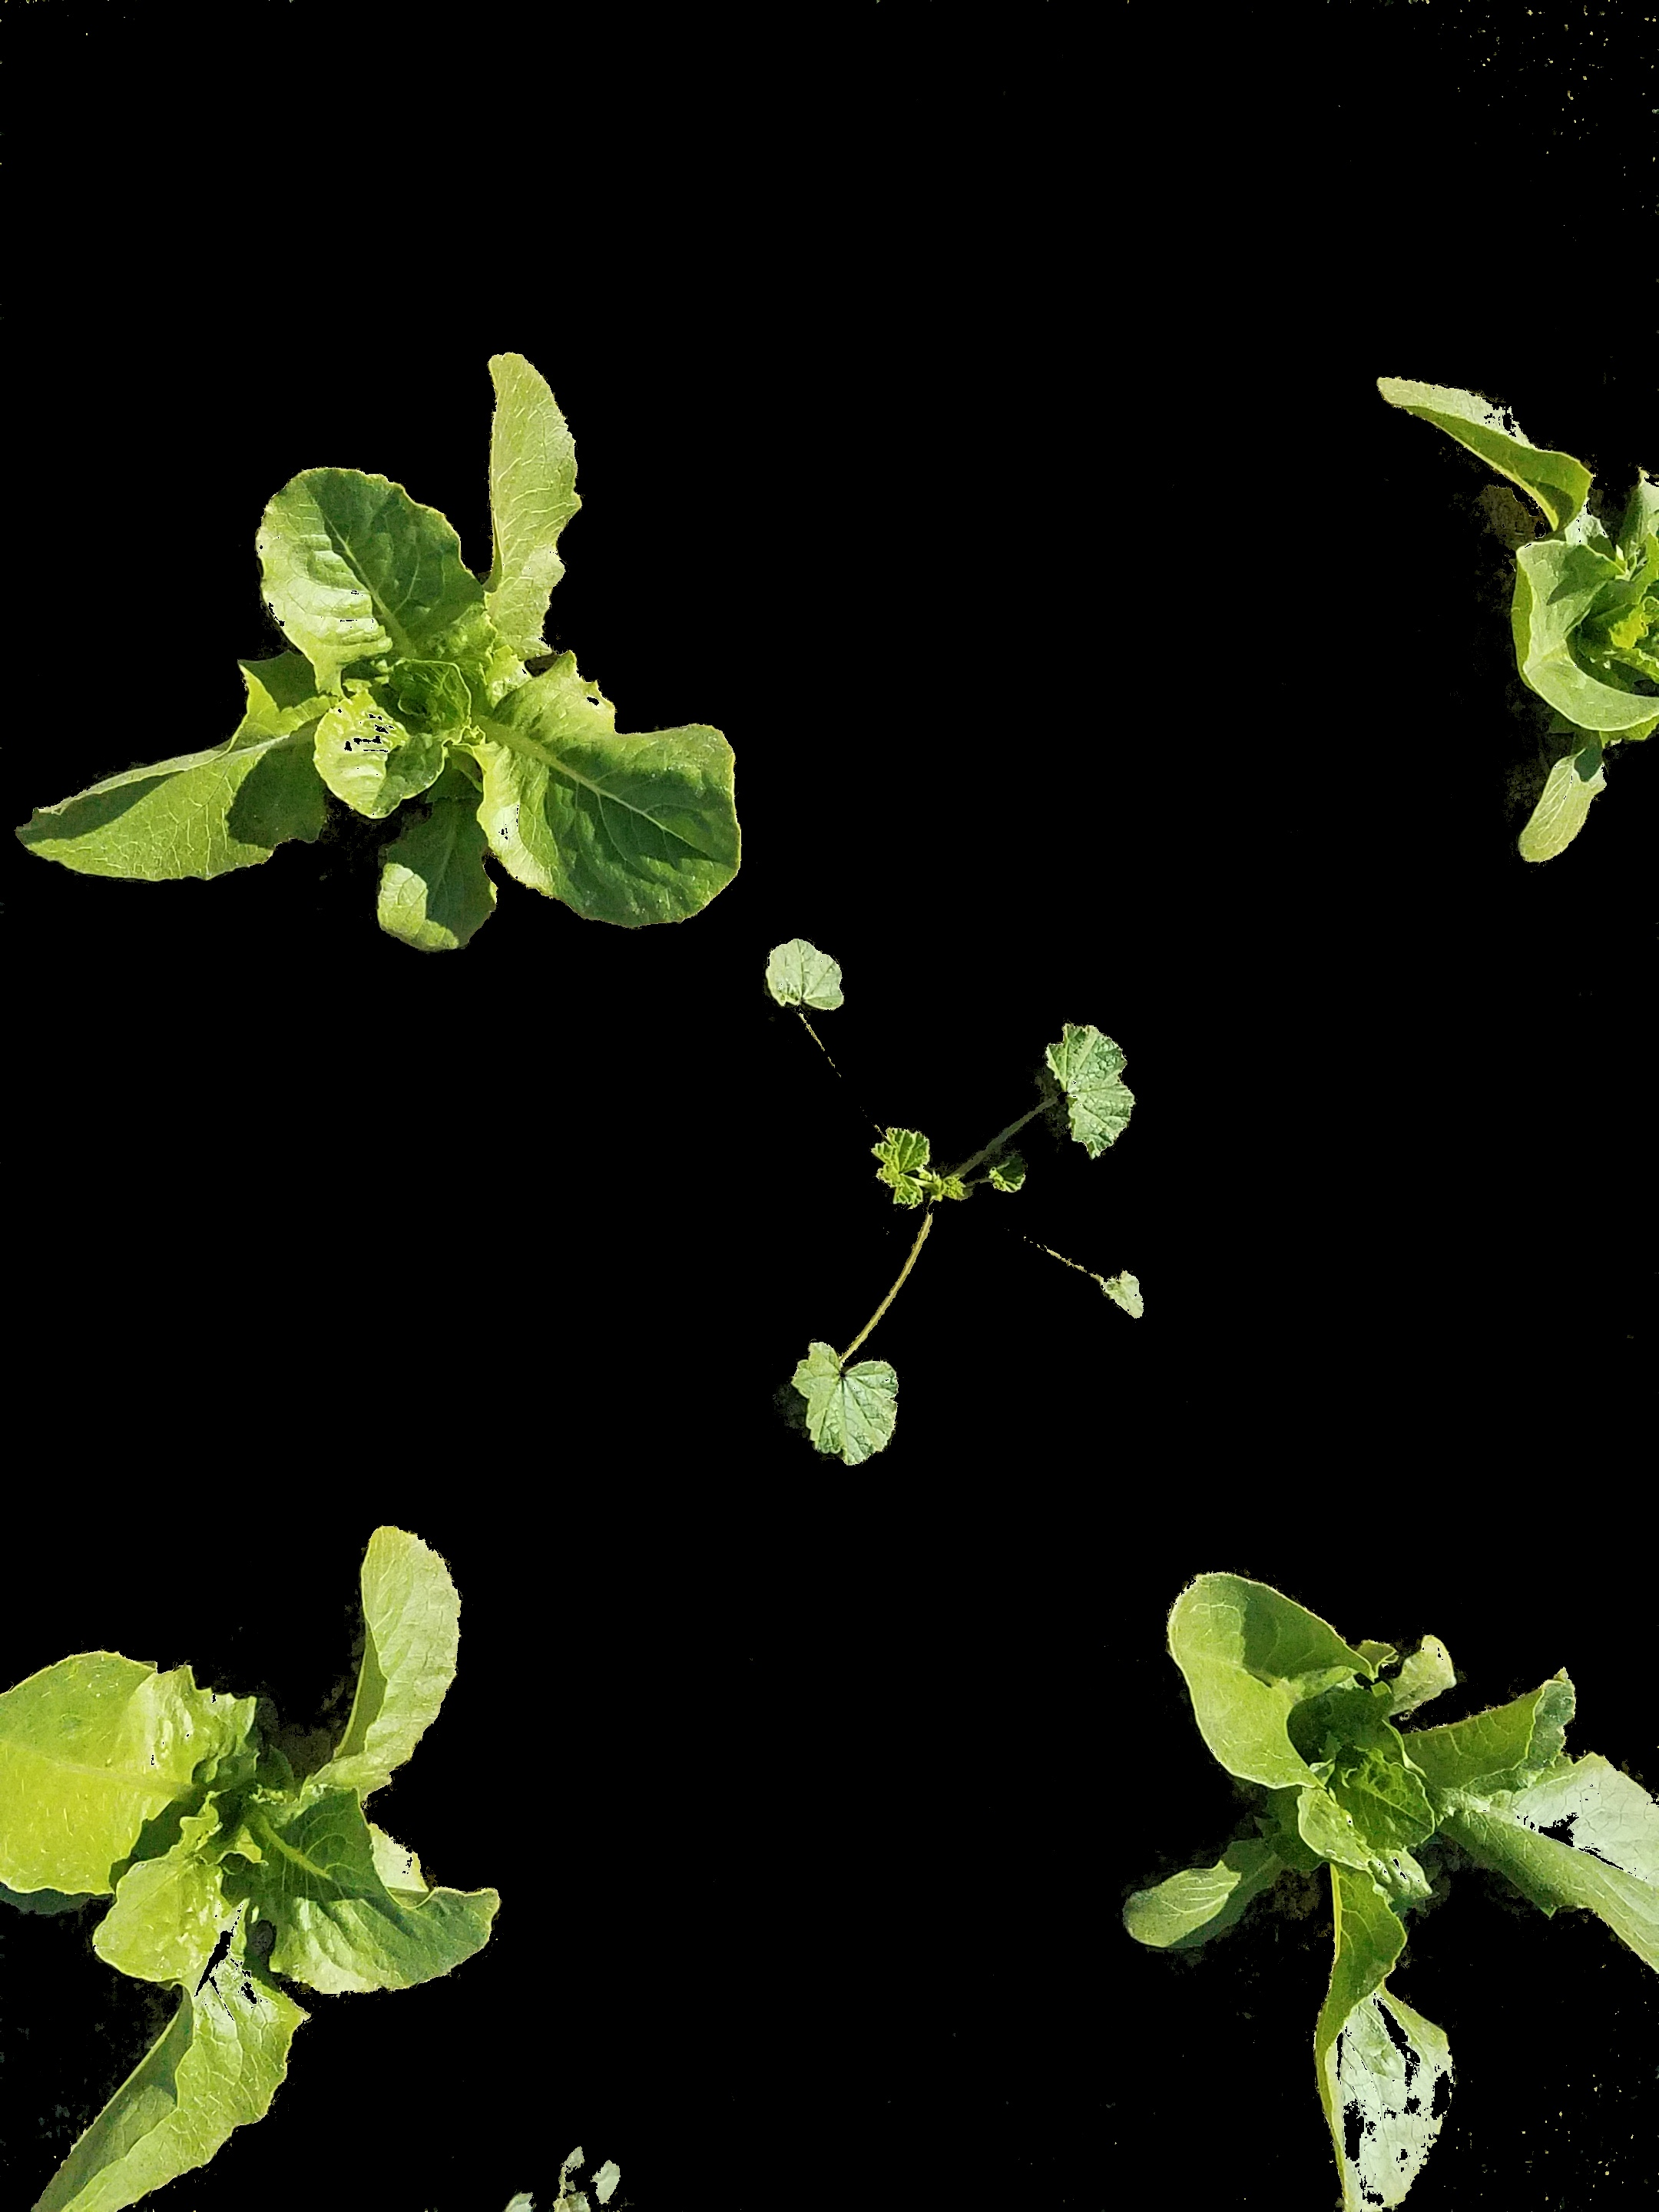
\includegraphics[width = 1.25in]{figures/20201117_112624-COM1.jpg} \label{fig:com1}} &
\subfloat[Com2]{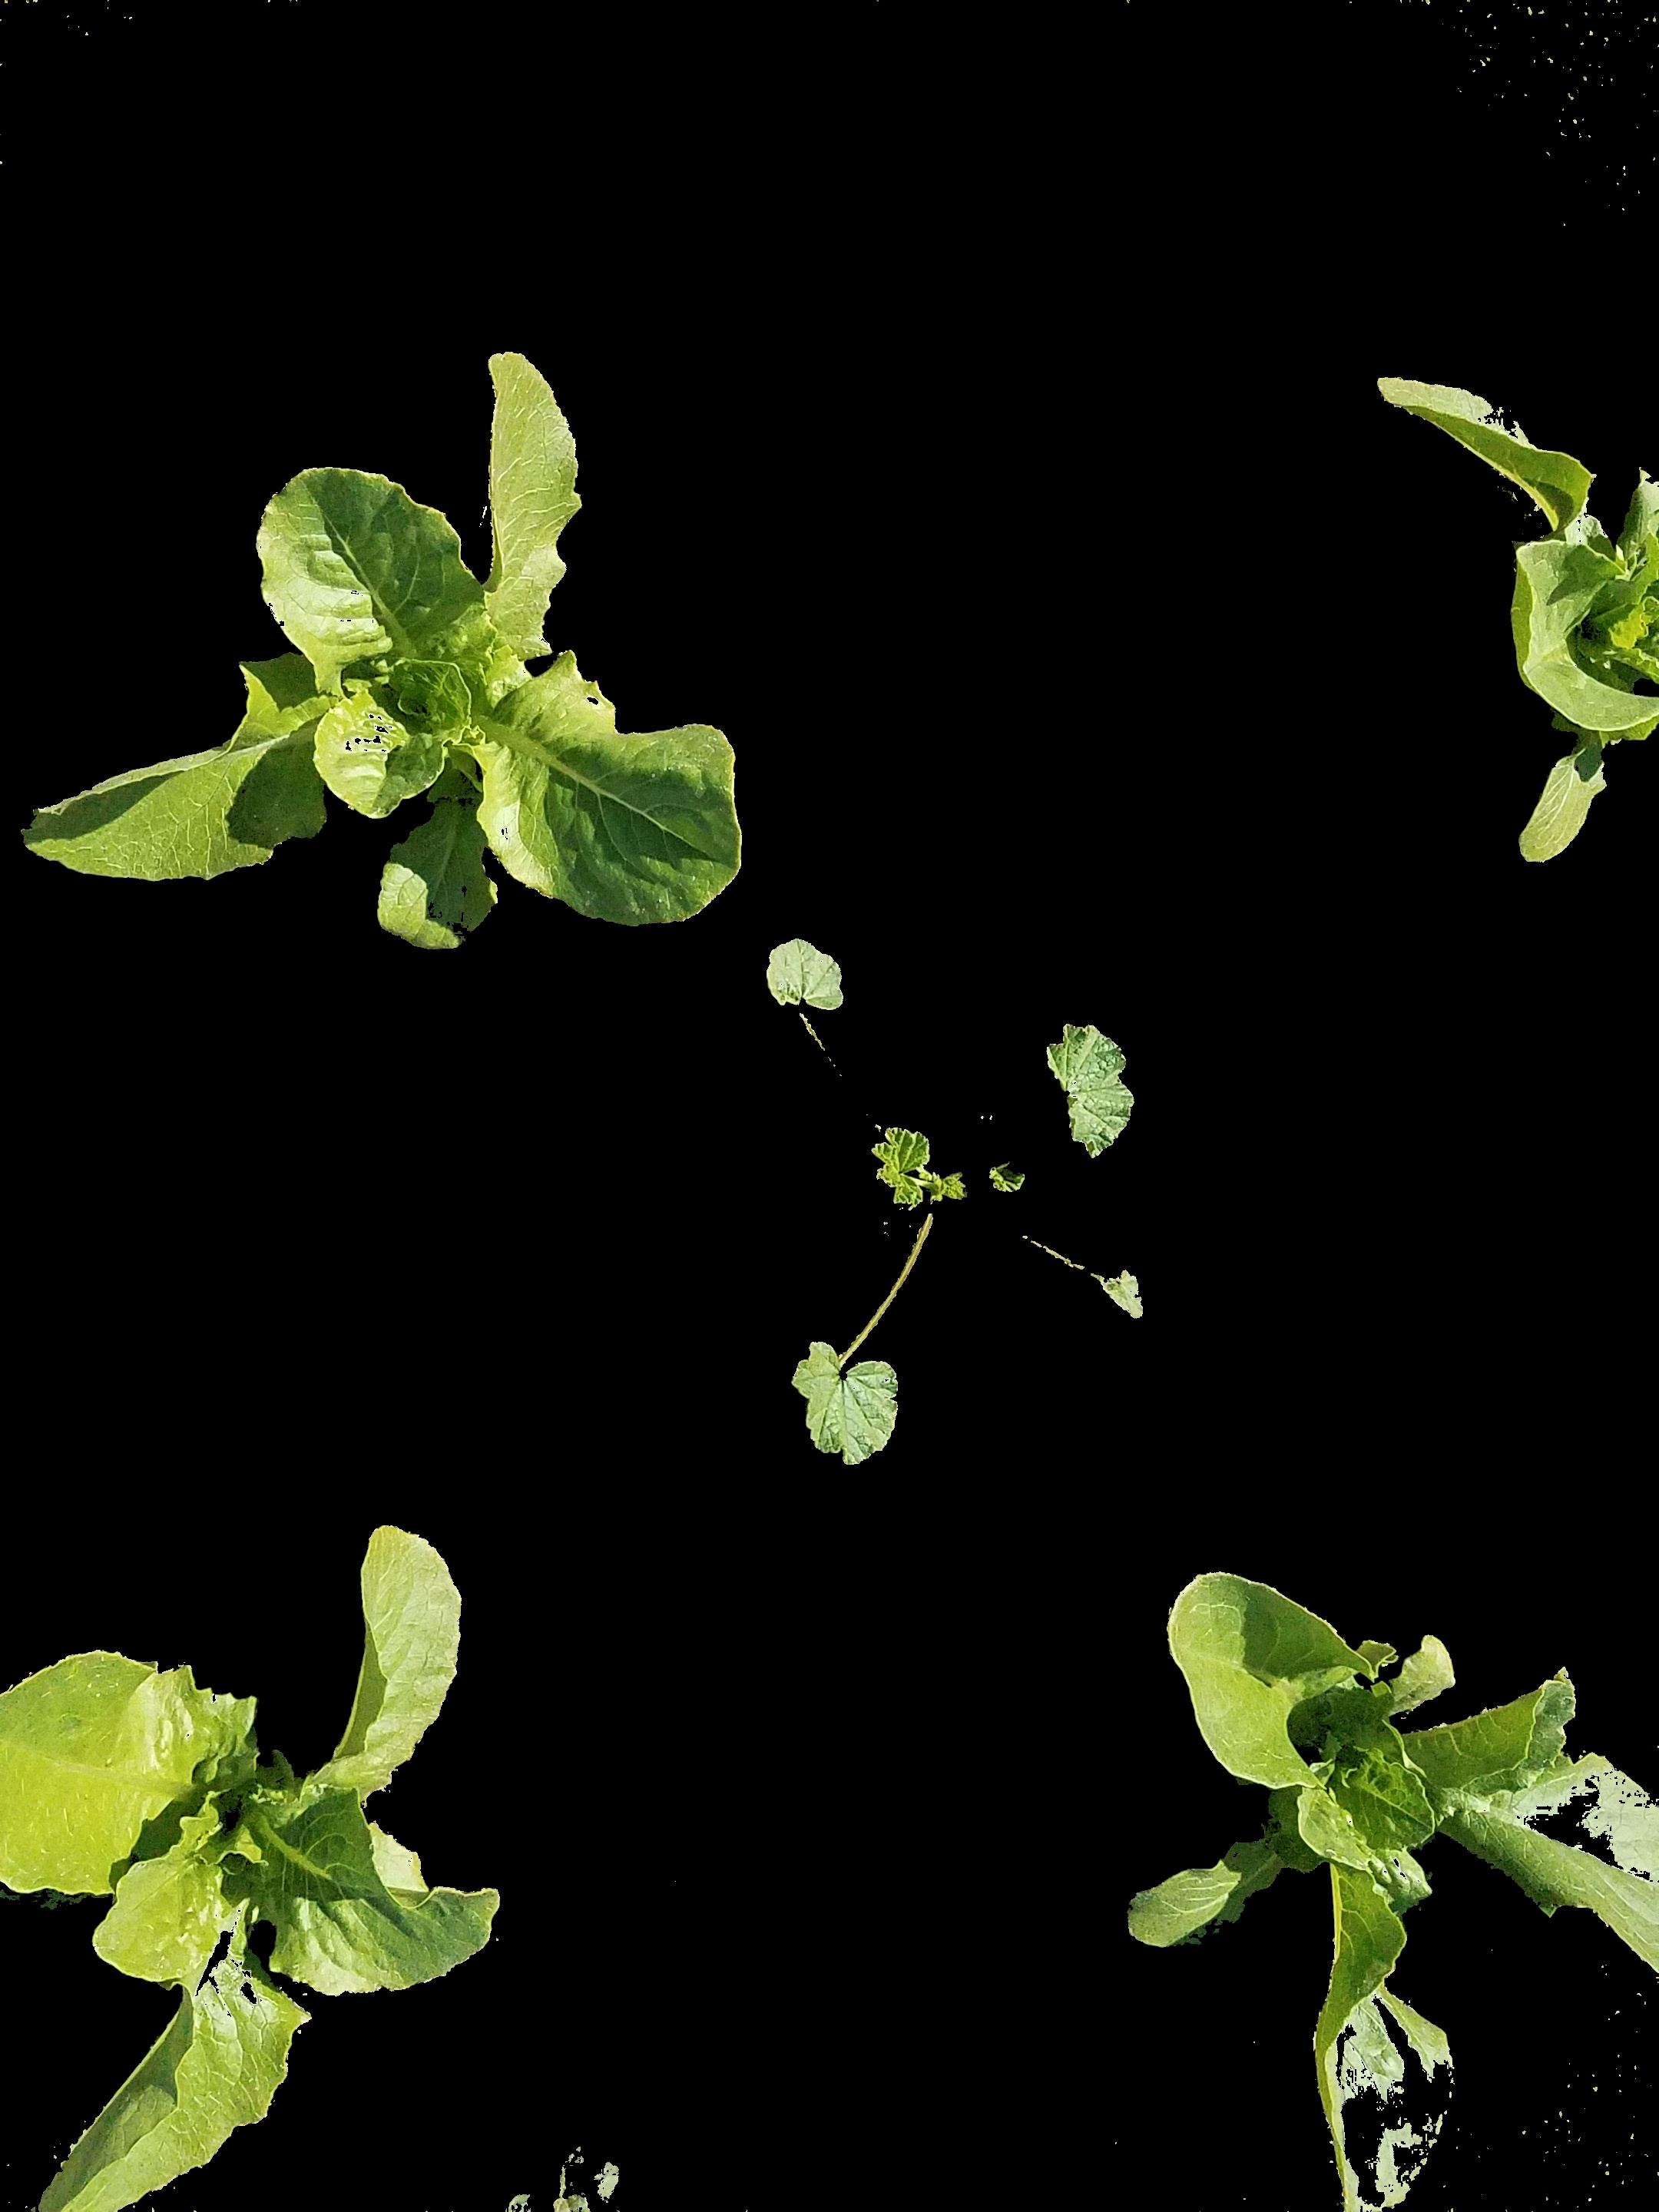
\includegraphics[width = 1.25in]{figures/20201117_112624-COM2.jpg} \label{fig:com2}}&
\subfloat[MEXG]{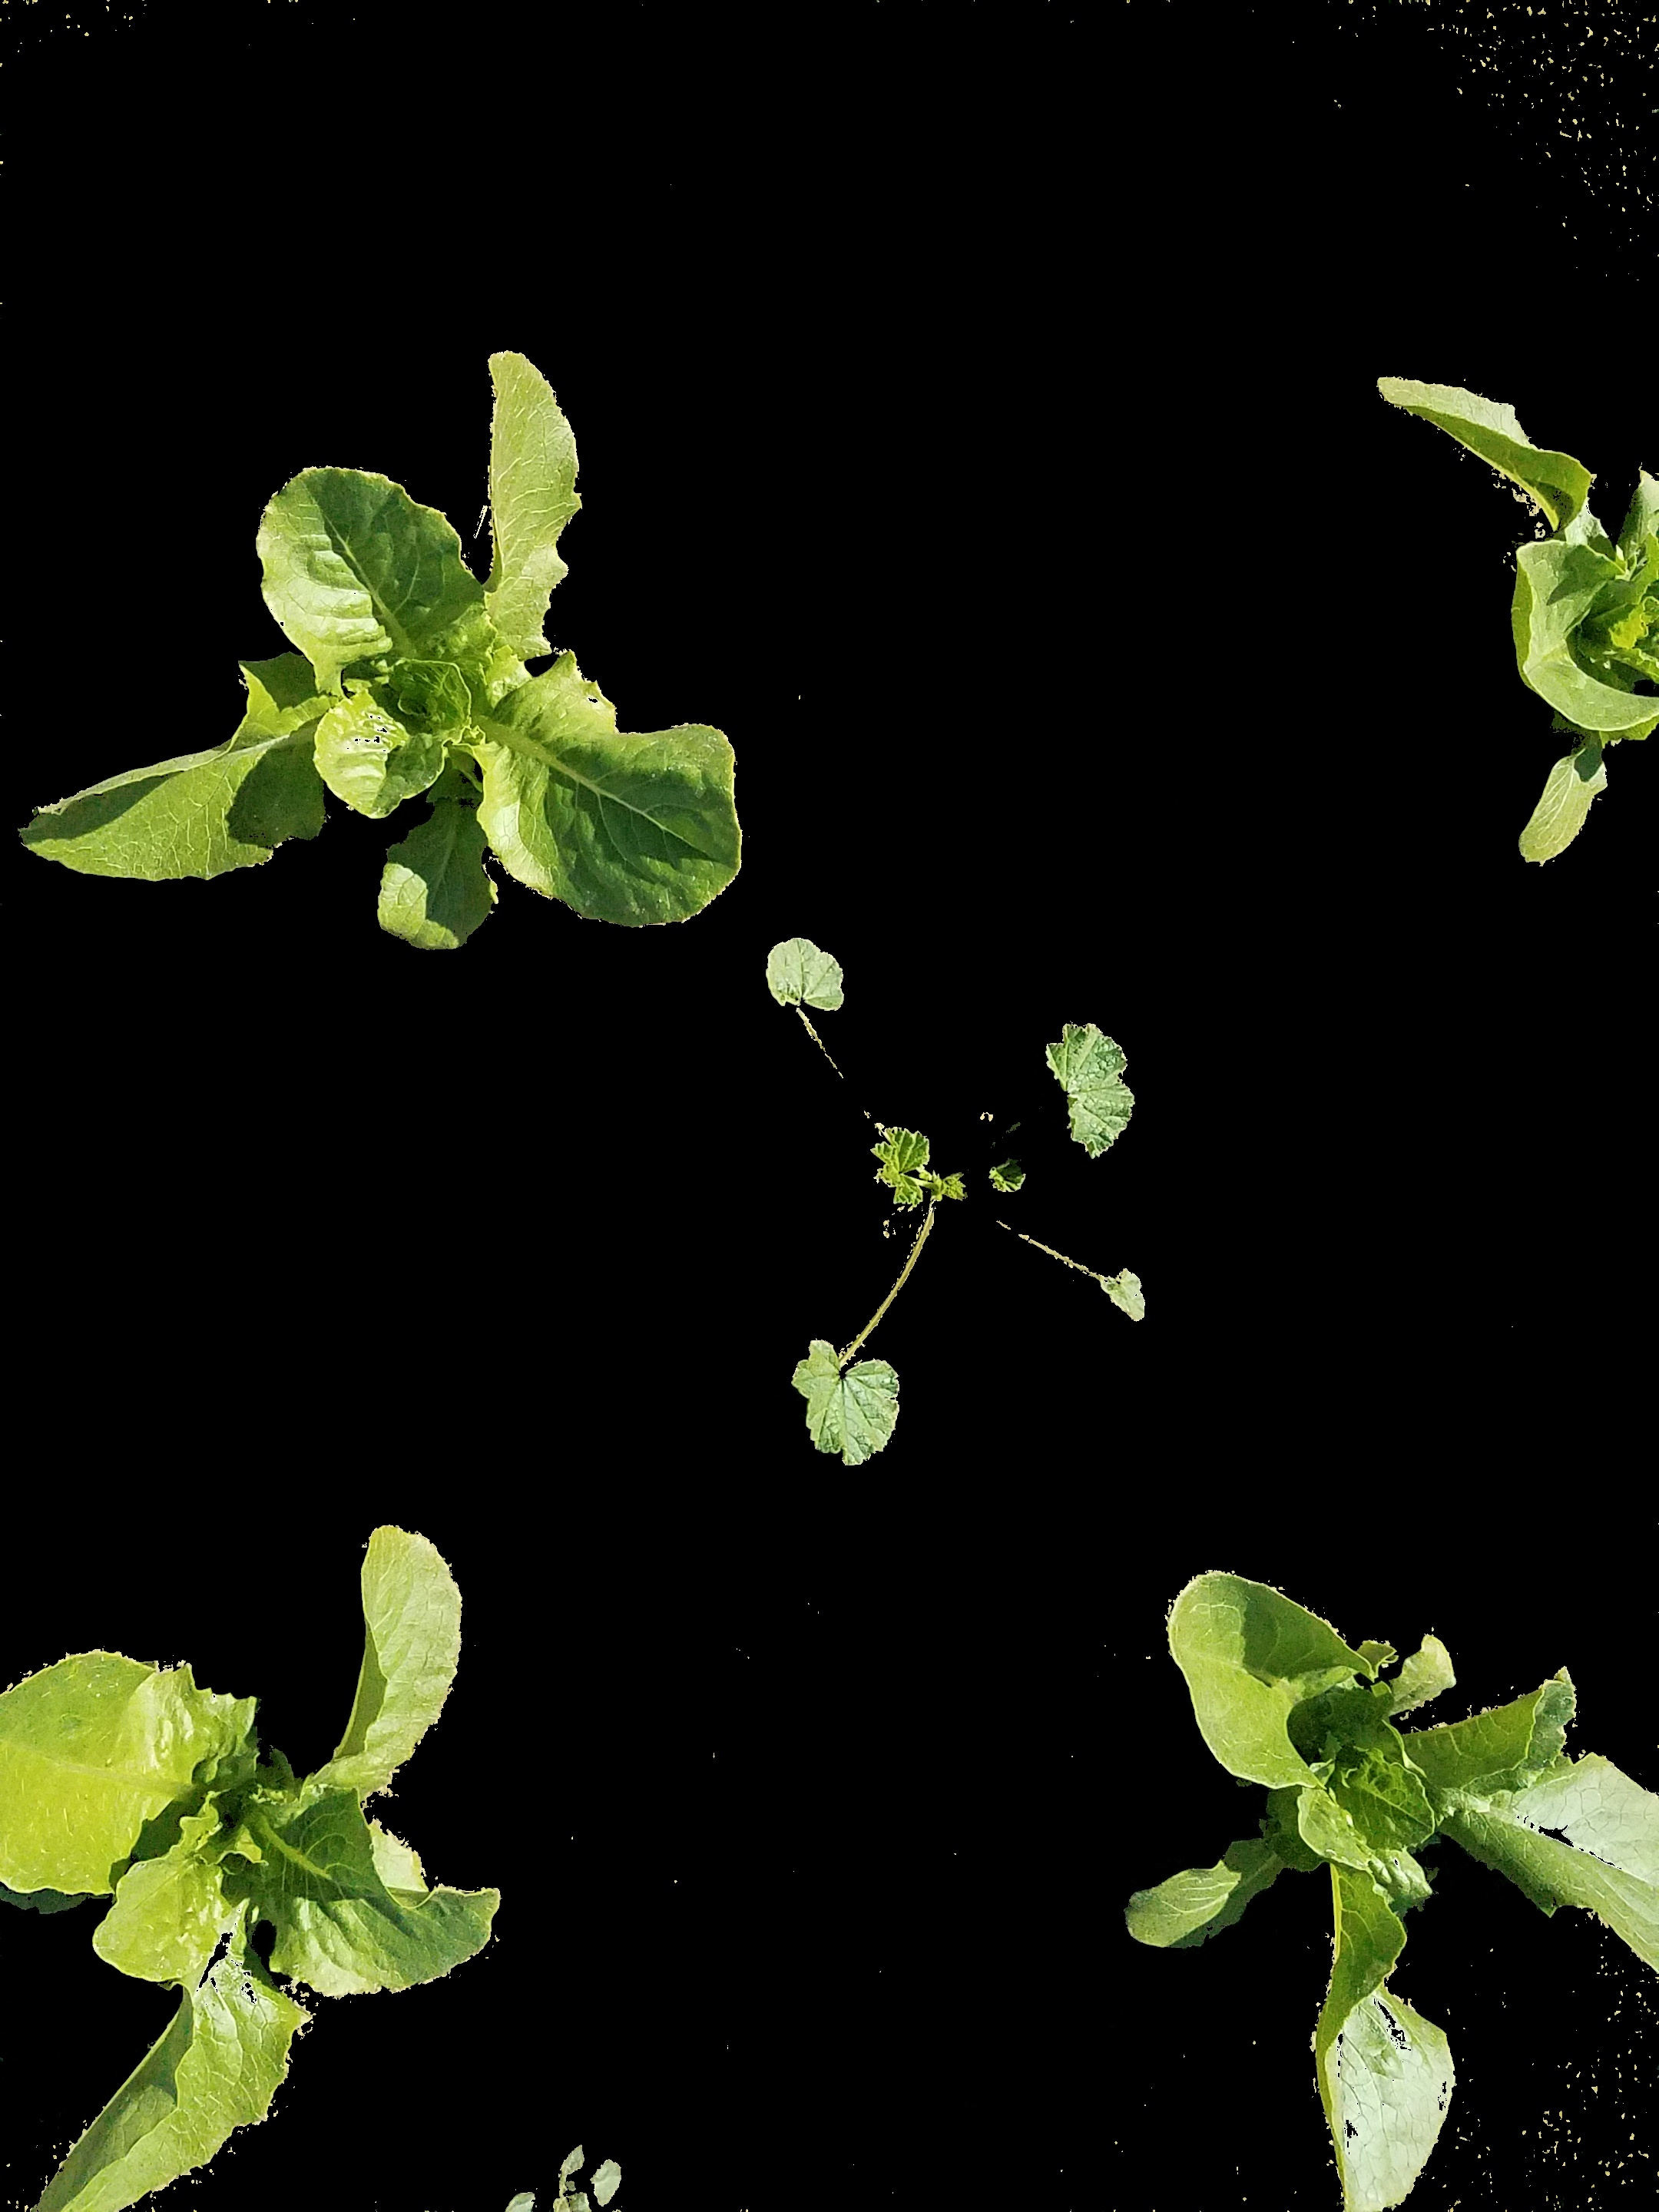
\includegraphics[width =1.25in]{figures/20201117_112624-MexG.jpg} \label{fig:mexg}} \\
\subfloat[TGI]{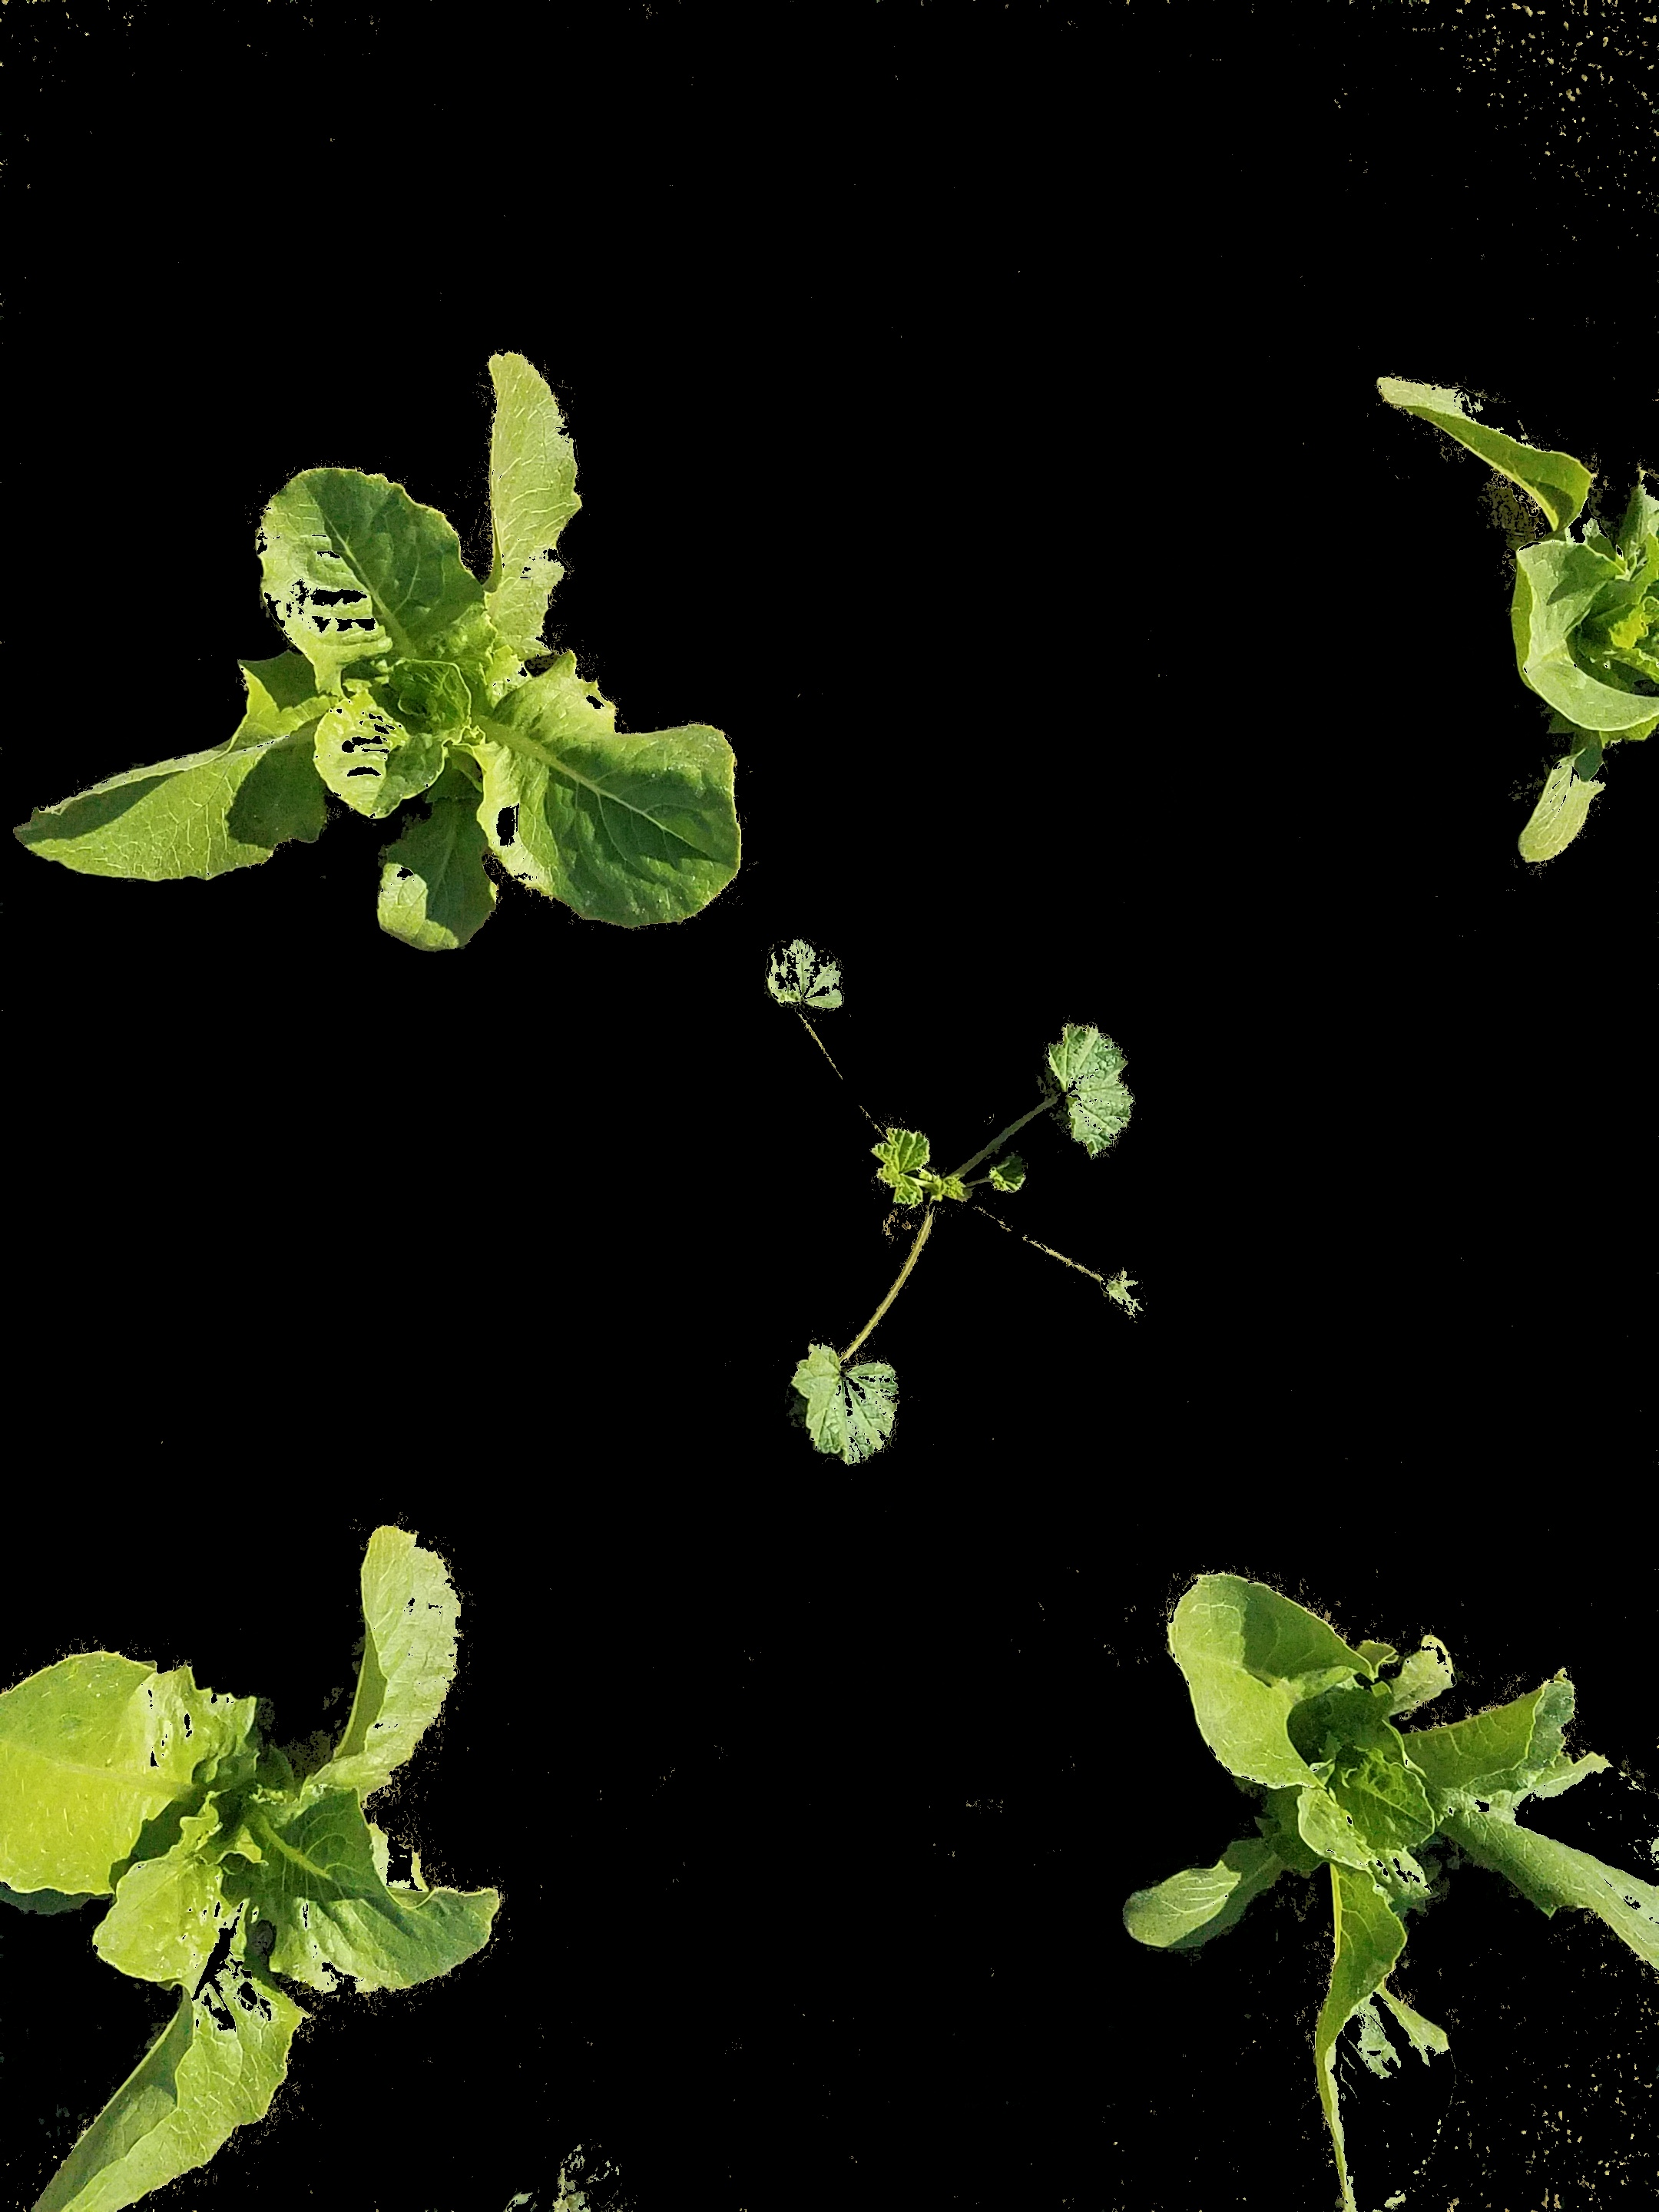
\includegraphics[width =1.25in]{figures/20201117_112624-TGI.jpg} \label{fig:tgi}} &
\subfloat[VEG]{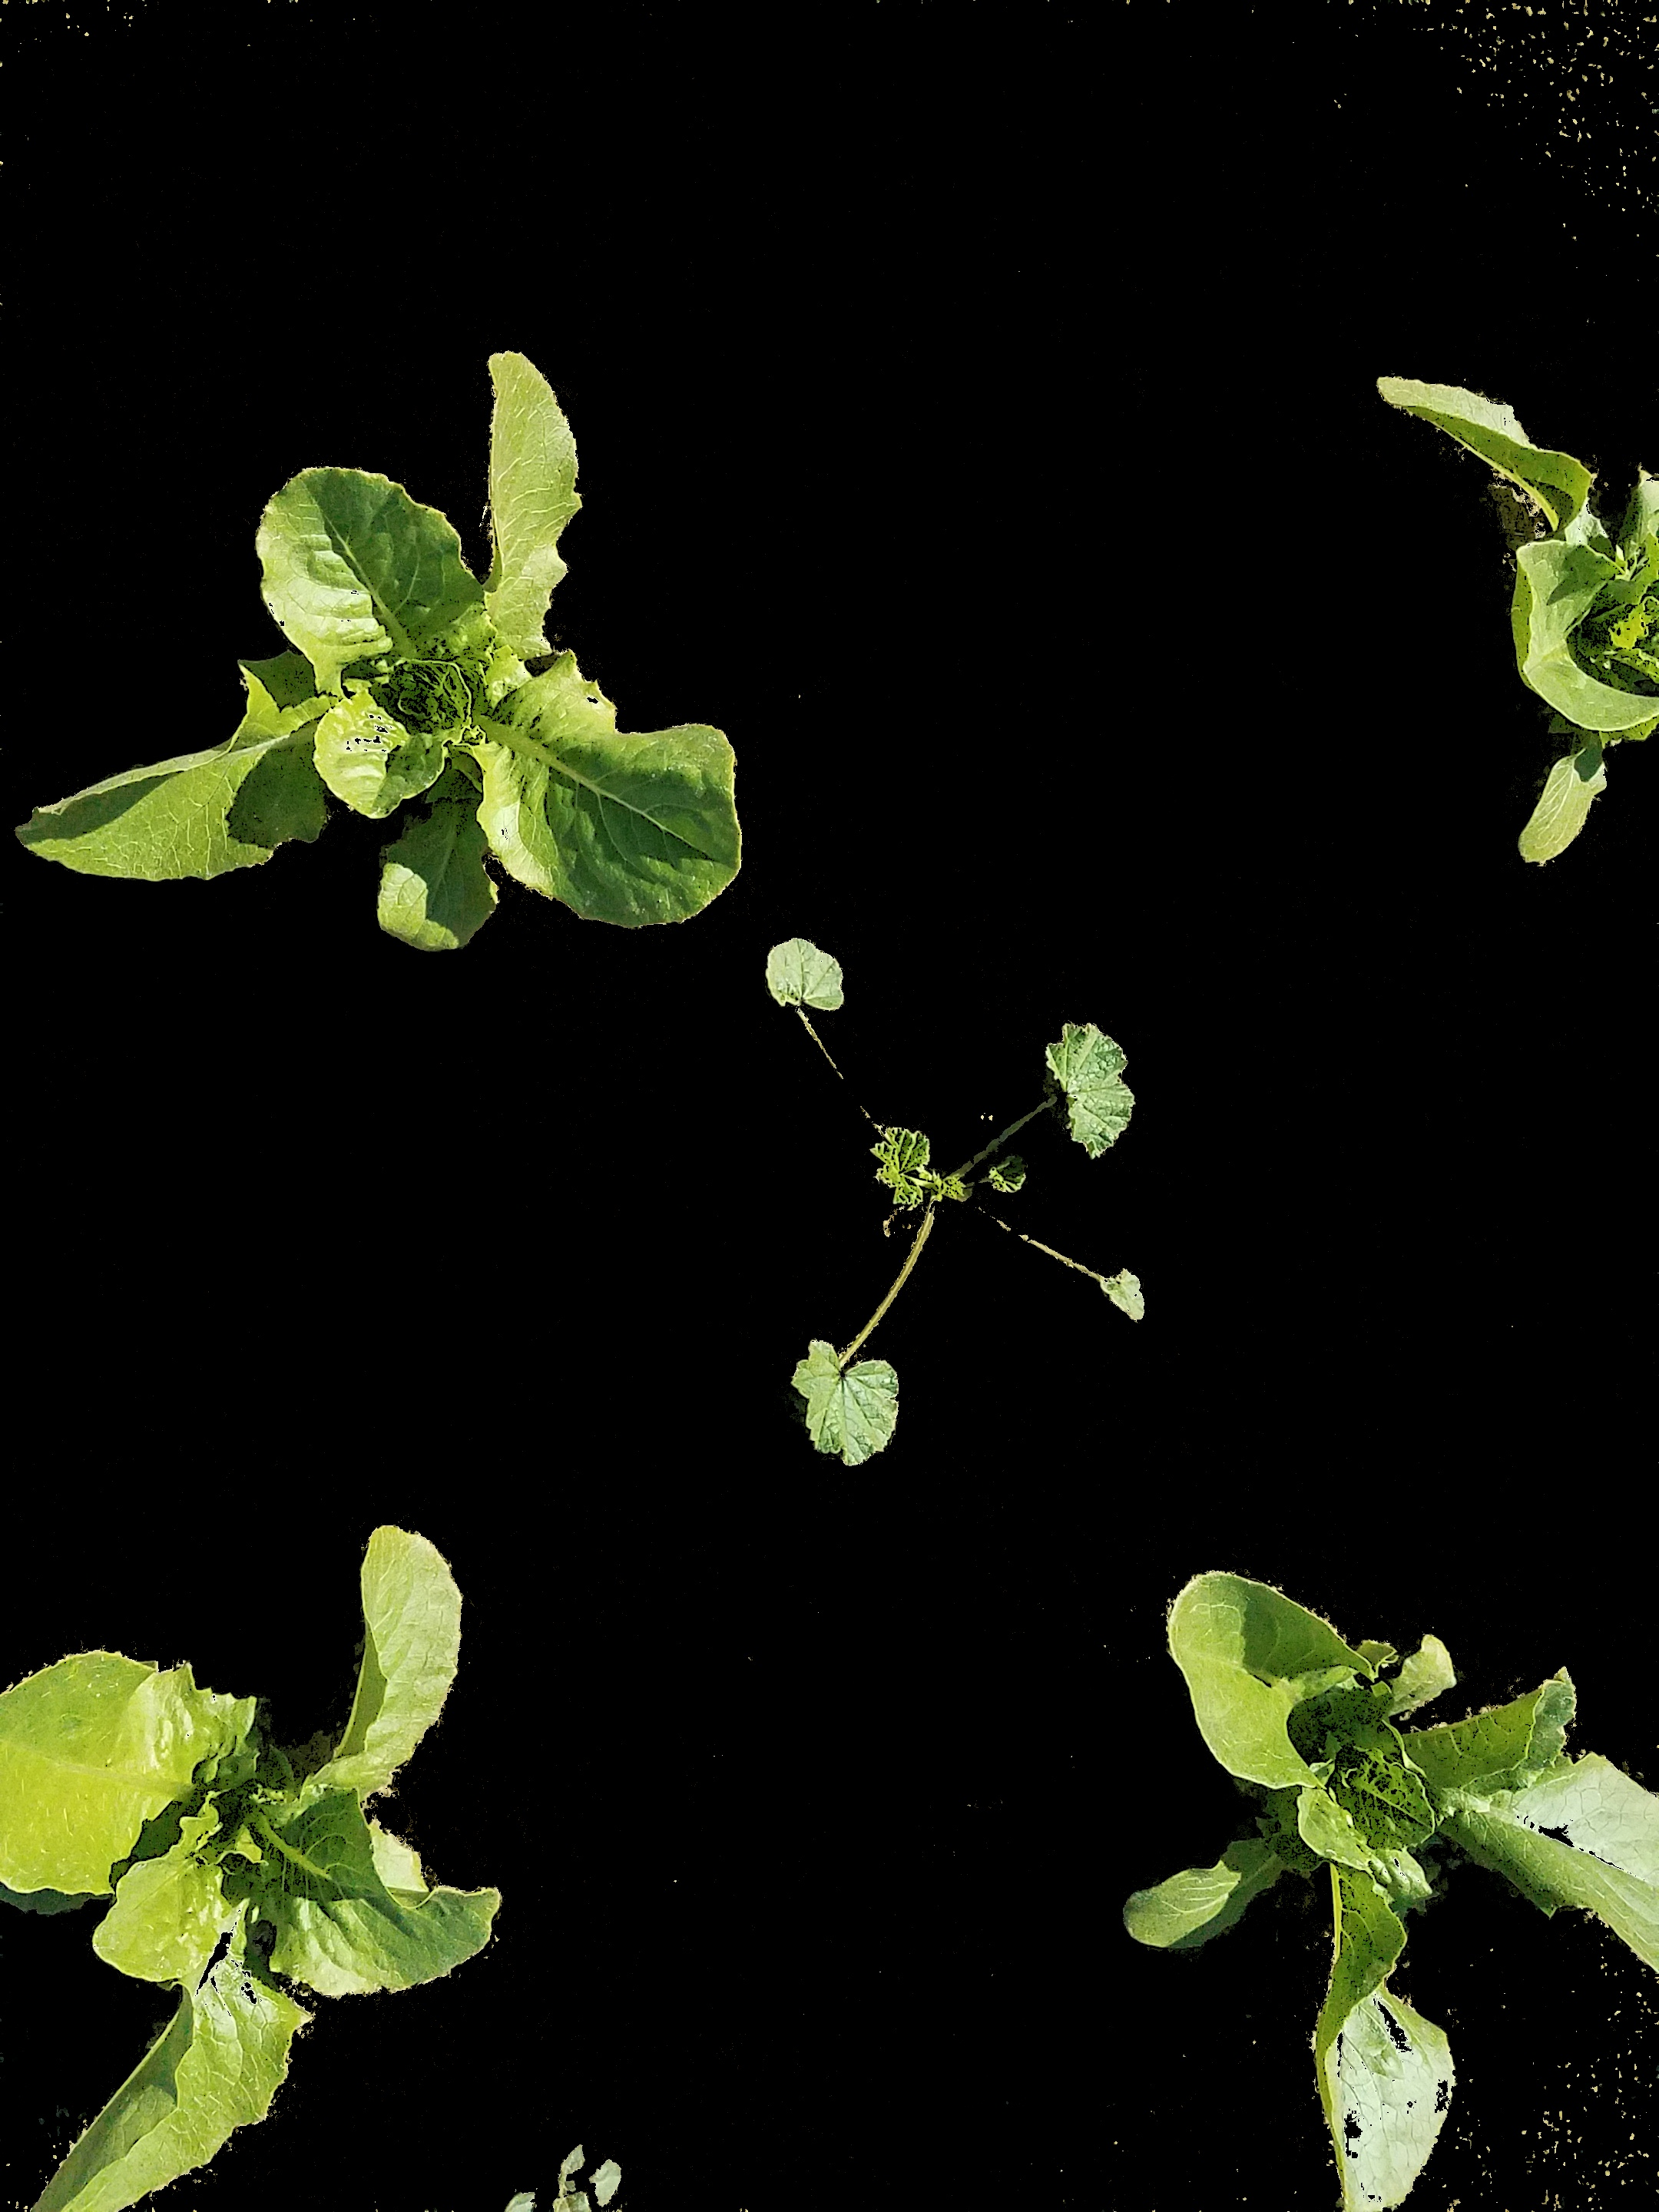
\includegraphics[width =1.25in]{figures/20201117_112624-VEG.jpg} \label{fig:veg}} &
\subfloat[Original]{\includegraphics[scale=0.0415,angle=270]{figures/20201117_112624.jpg} \label{fig:original}} \\
\end{tabular}
\caption[Results of various visible-light image segmentation techniques]{Various visible-light image segmentation techniques (See Table \ref{table:segmentation} for details). At first glance, many of the segmentation algorithms produce similar results, but some of the methods are not sensitive to less green portions of the plants -- slender stems. Contrast the results seen in \ref{fig:exr} and \ref{fig:mexg}, with the slender stems of the plant in the middle of the image not present in the result of the former.}
\label{figure:results}
\end{figure}

There are two sorts of mistakes encountered in segmentation, as there are only two sorts of things in the image: things that are vegetation (crop and weeds) and things that aren't (typically, the ground). Omission of a crop leaf is apparent in Figure \ref{fig:ndi}, showing the result of using NDI.  The center plant is only partially visible. Contrast that with the result shown in Figures \ref{fig:hi} and  \ref{fig:hv}, where the ground is featured. This case may be due to the shadow of the plant containing too much green as sunlight passes through the leaf. Figure \ref{fig:overlay} illustrates the effects of the index and errors -- of special note here is the error that is shown in the upper right-hand portion of Figure \ref{fig:overlay-cive}. Applying the NDI mask produces the errors discussed previously -- the leaf shadow is identified as vegetation. The evaluation of errors in index-based approaches is illustrated 

% Bar chart produced with this command
%  python evaluate-masks.py -i ../lib/mask.jpg -t ../lib/testing/20201117_112624
\begin{figure}[h]
	\centering
	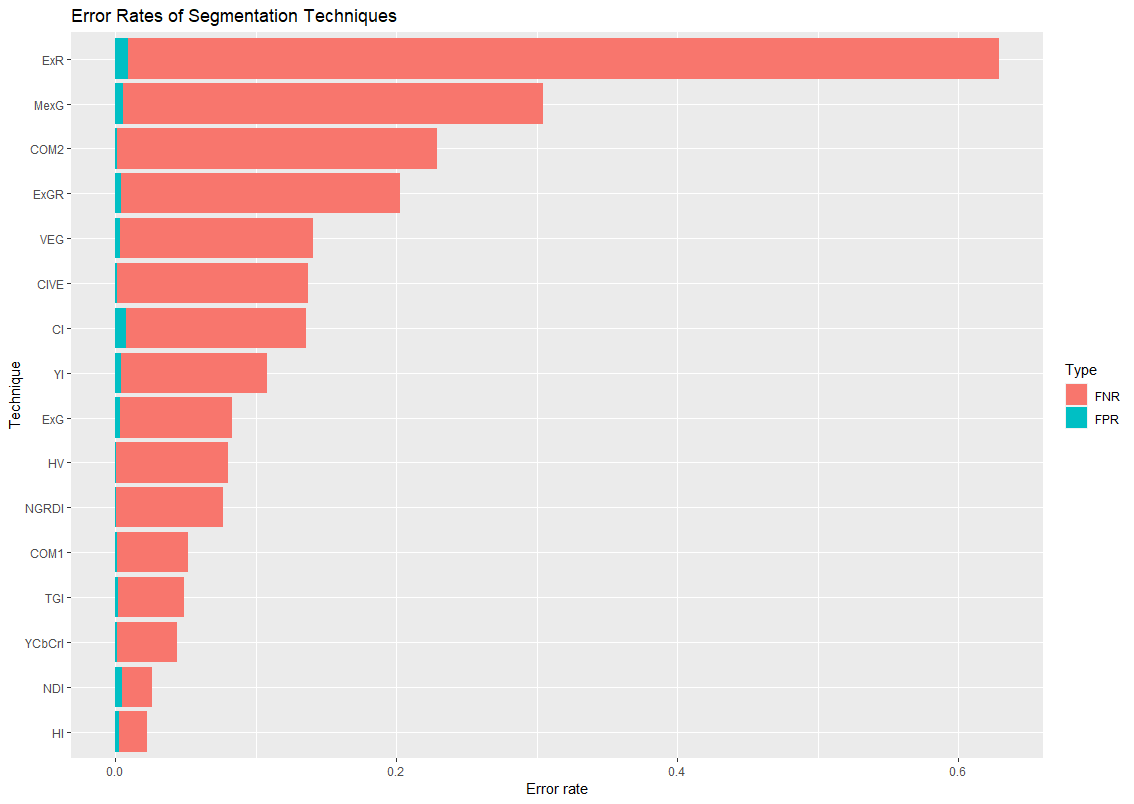
\includegraphics[width=.75\linewidth]{figures/segmentation-error-rates.png}
	\caption[Error rates of segmentation algorithms]{Average error rates for the images. Type I (Vegetation identified as ground) and Type II (Ground identified as vegetation) error are summarized by this figure. Of special note here are the errors encountered with NRGDI and HI approaches, as they represent clear differences in errors. The majority of the errors shown by the HI index mistakenly shows the ground as vegetation, with NDGRI  doing the opposite, hiding vegetation.}
	\label{fig:segmentation-errors}
\end{figure}

\begin{figure}[H]
\centering
\begin{tabular}{ccc}
	\subfloat[CIElab]{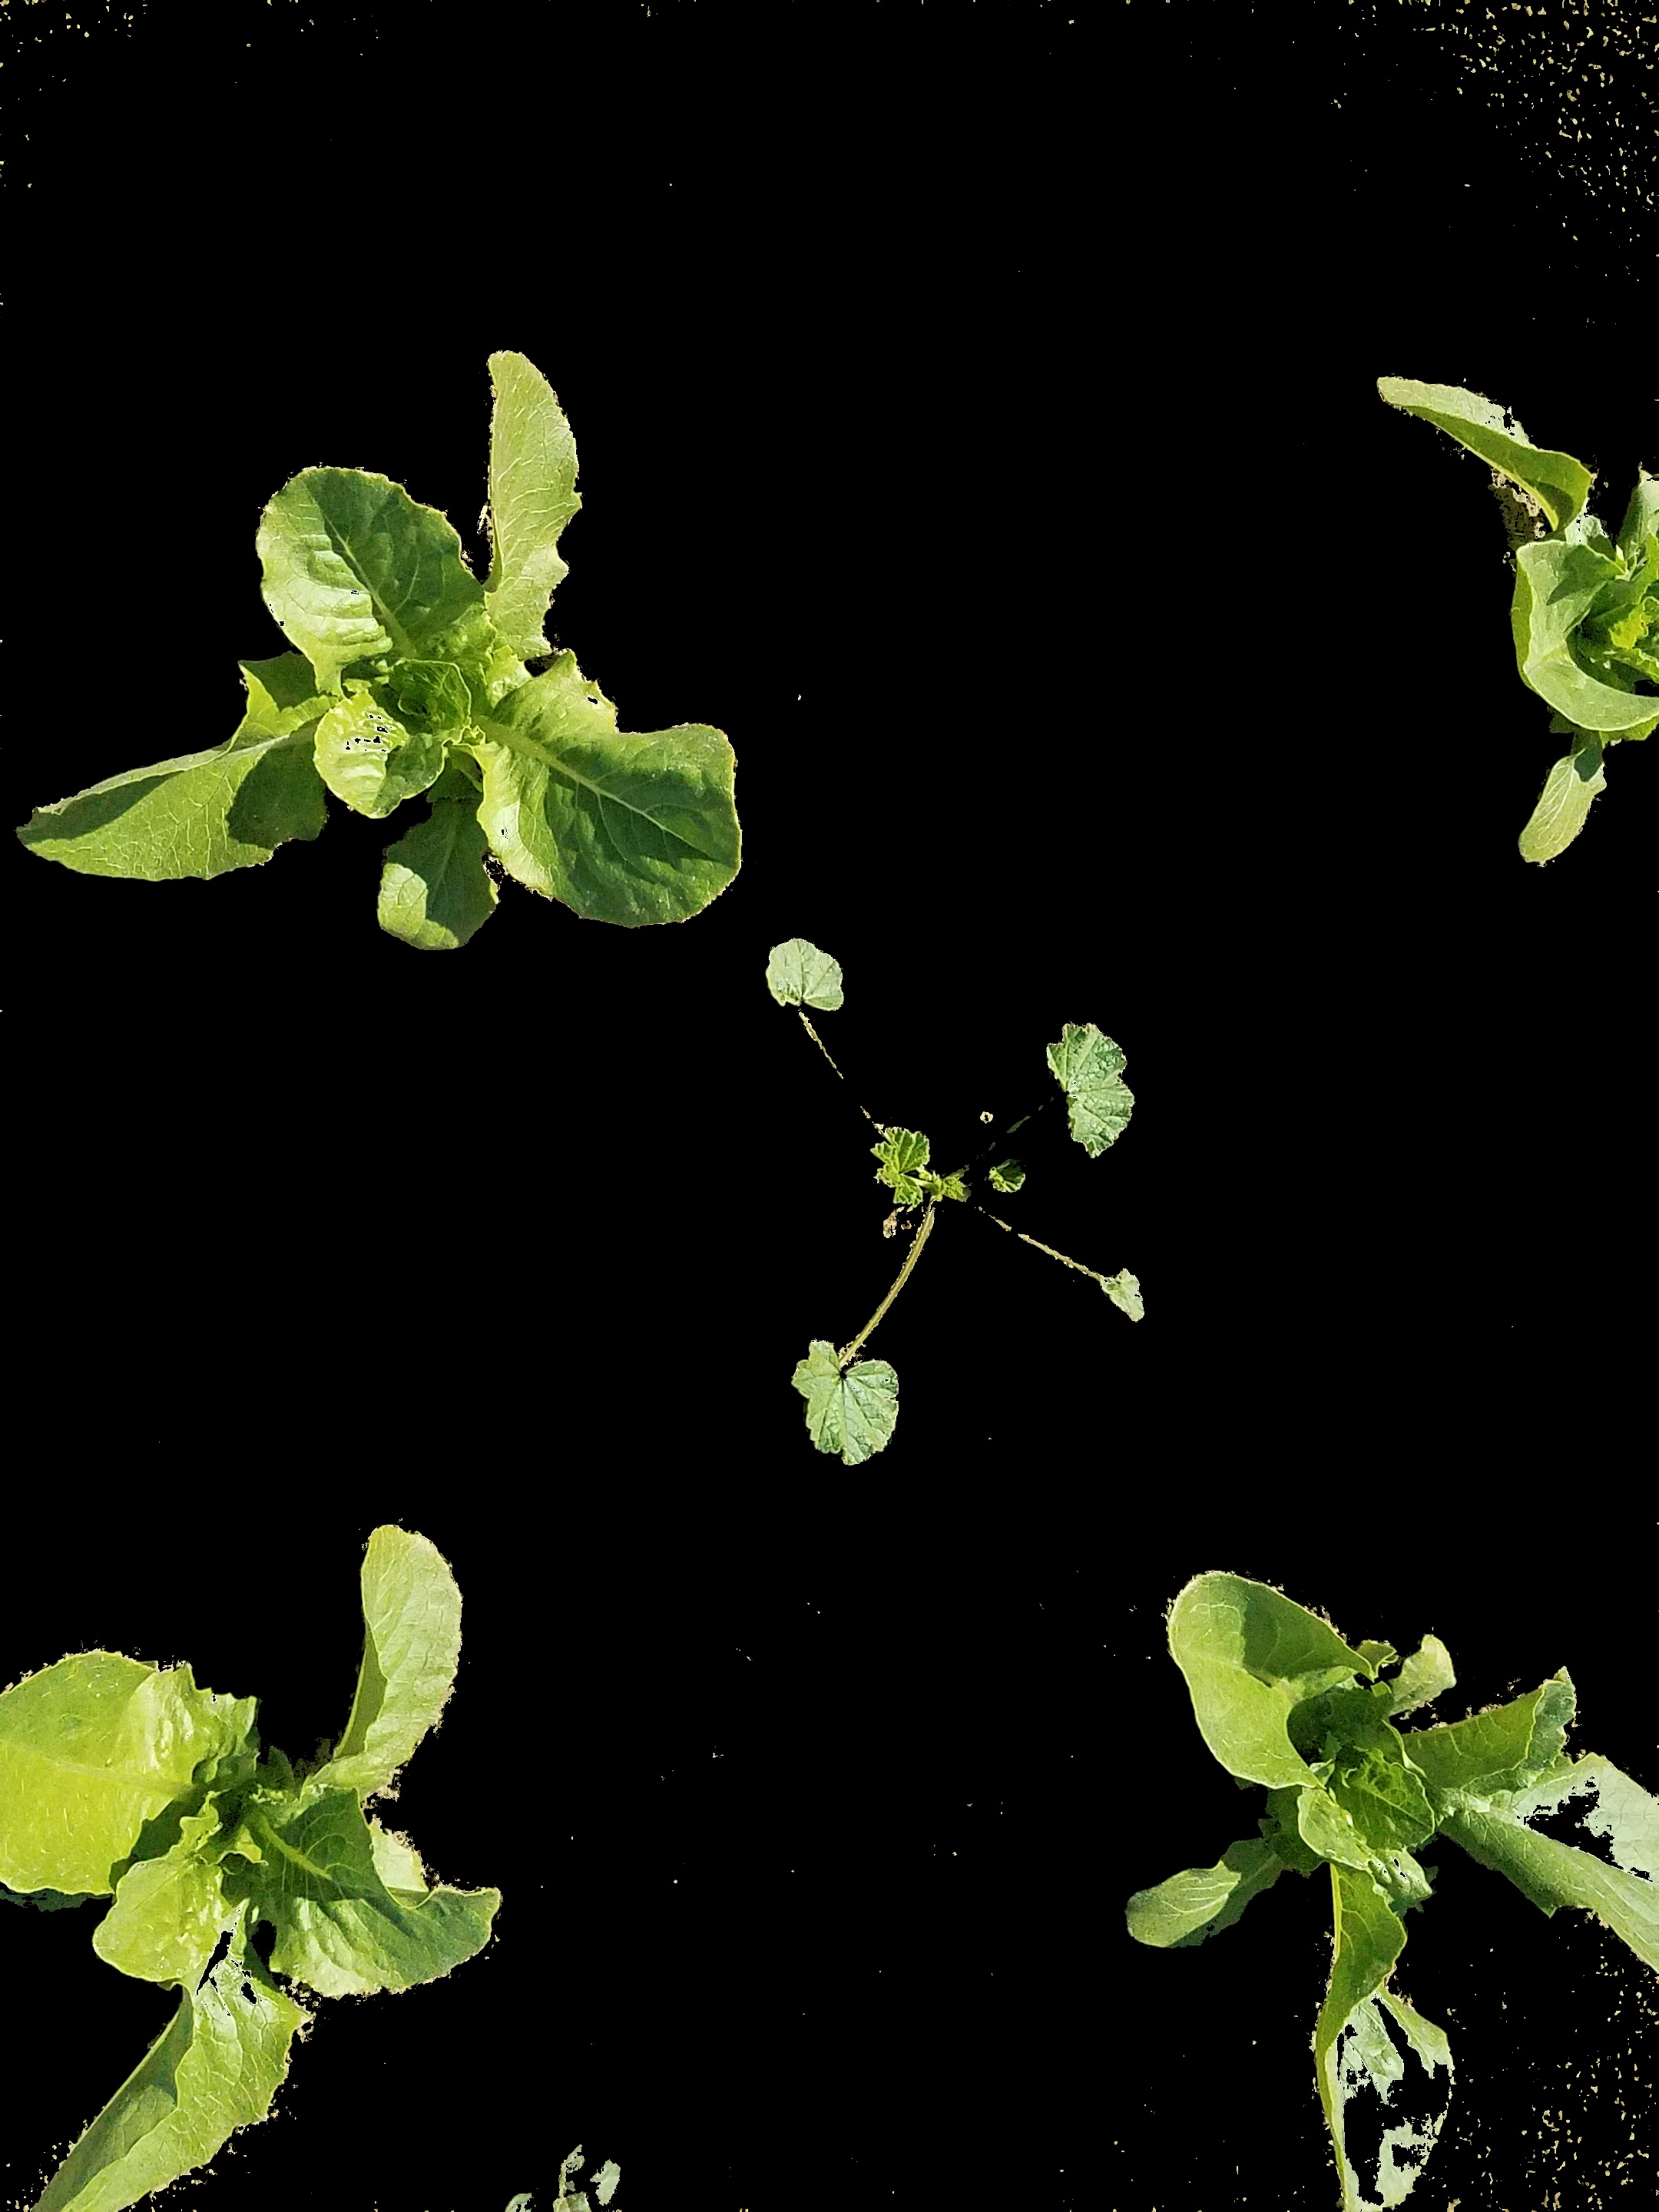
\includegraphics[width = 1.25in]{figures/20201117_112624-CI.jpg} \label{fig:ci}} &
	\subfloat[HSI]{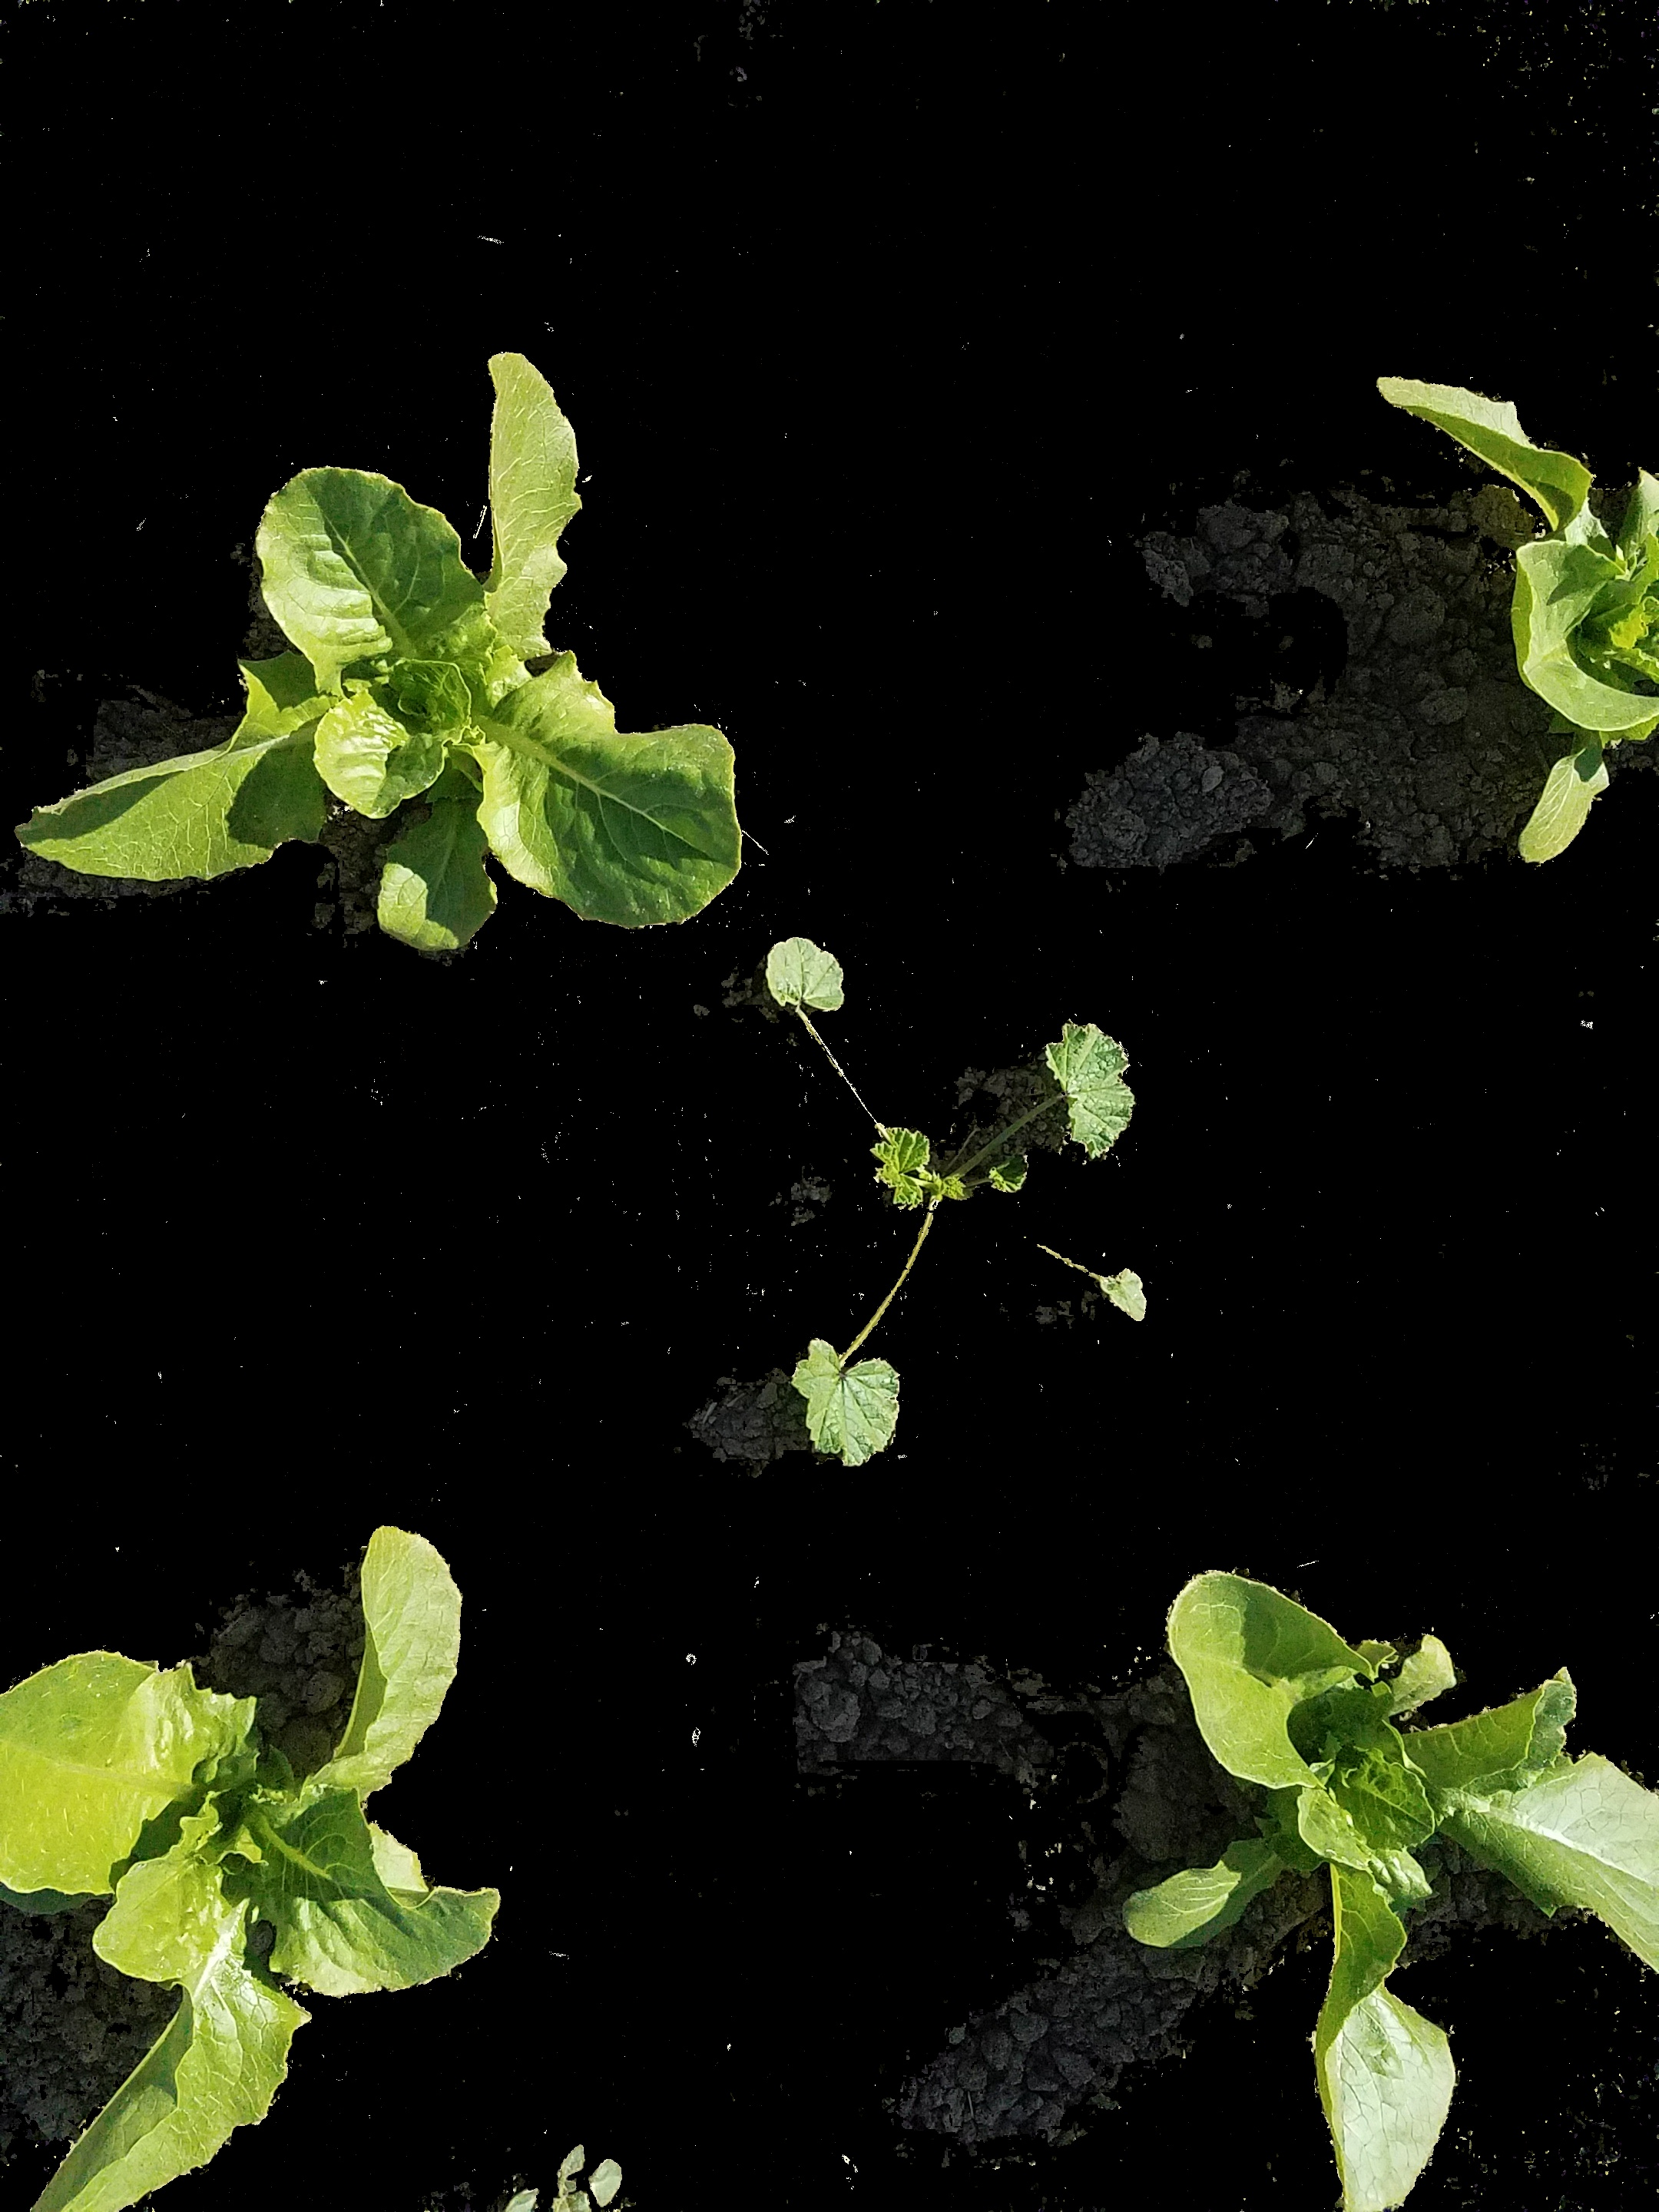
\includegraphics[width = 1.25in]{figures/20201117_112624-HI.jpg} \label{fig:hi}} &
	\subfloat[HSV]{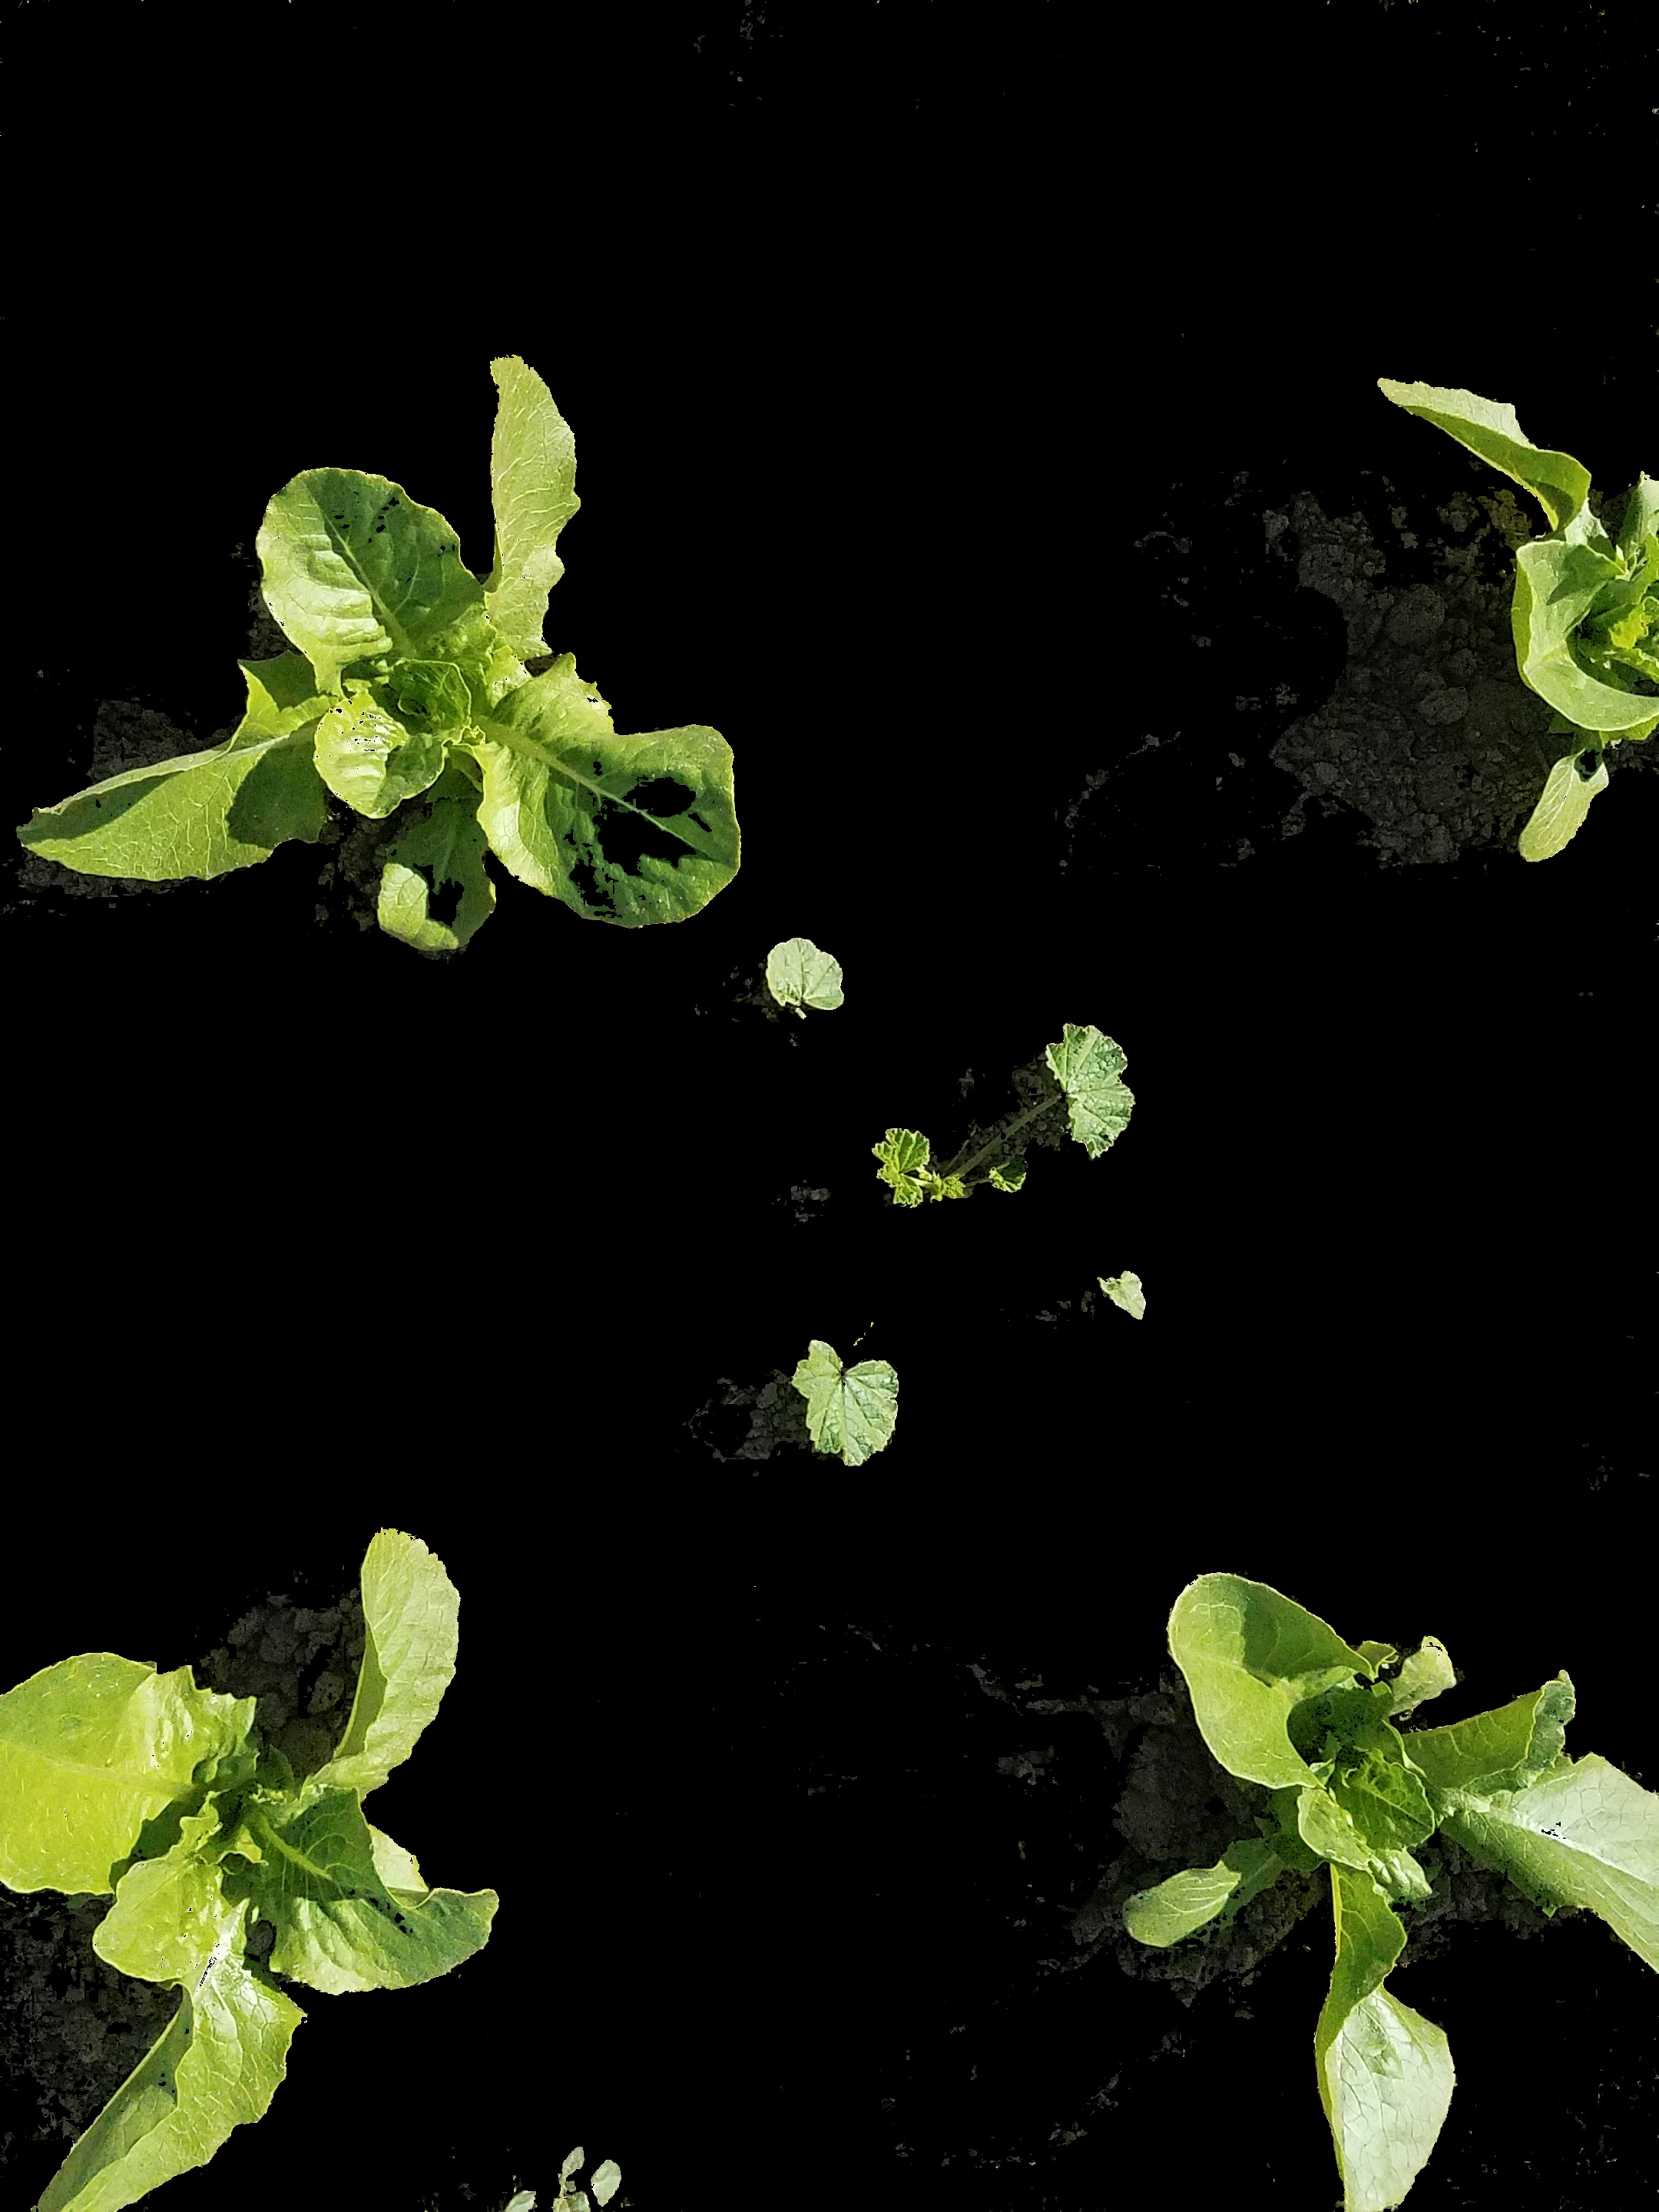
\includegraphics[width = 1.25in]{figures/20201117_112624-HV.jpg} \label{fig:hv}} \\
	\subfloat[YCbCr]{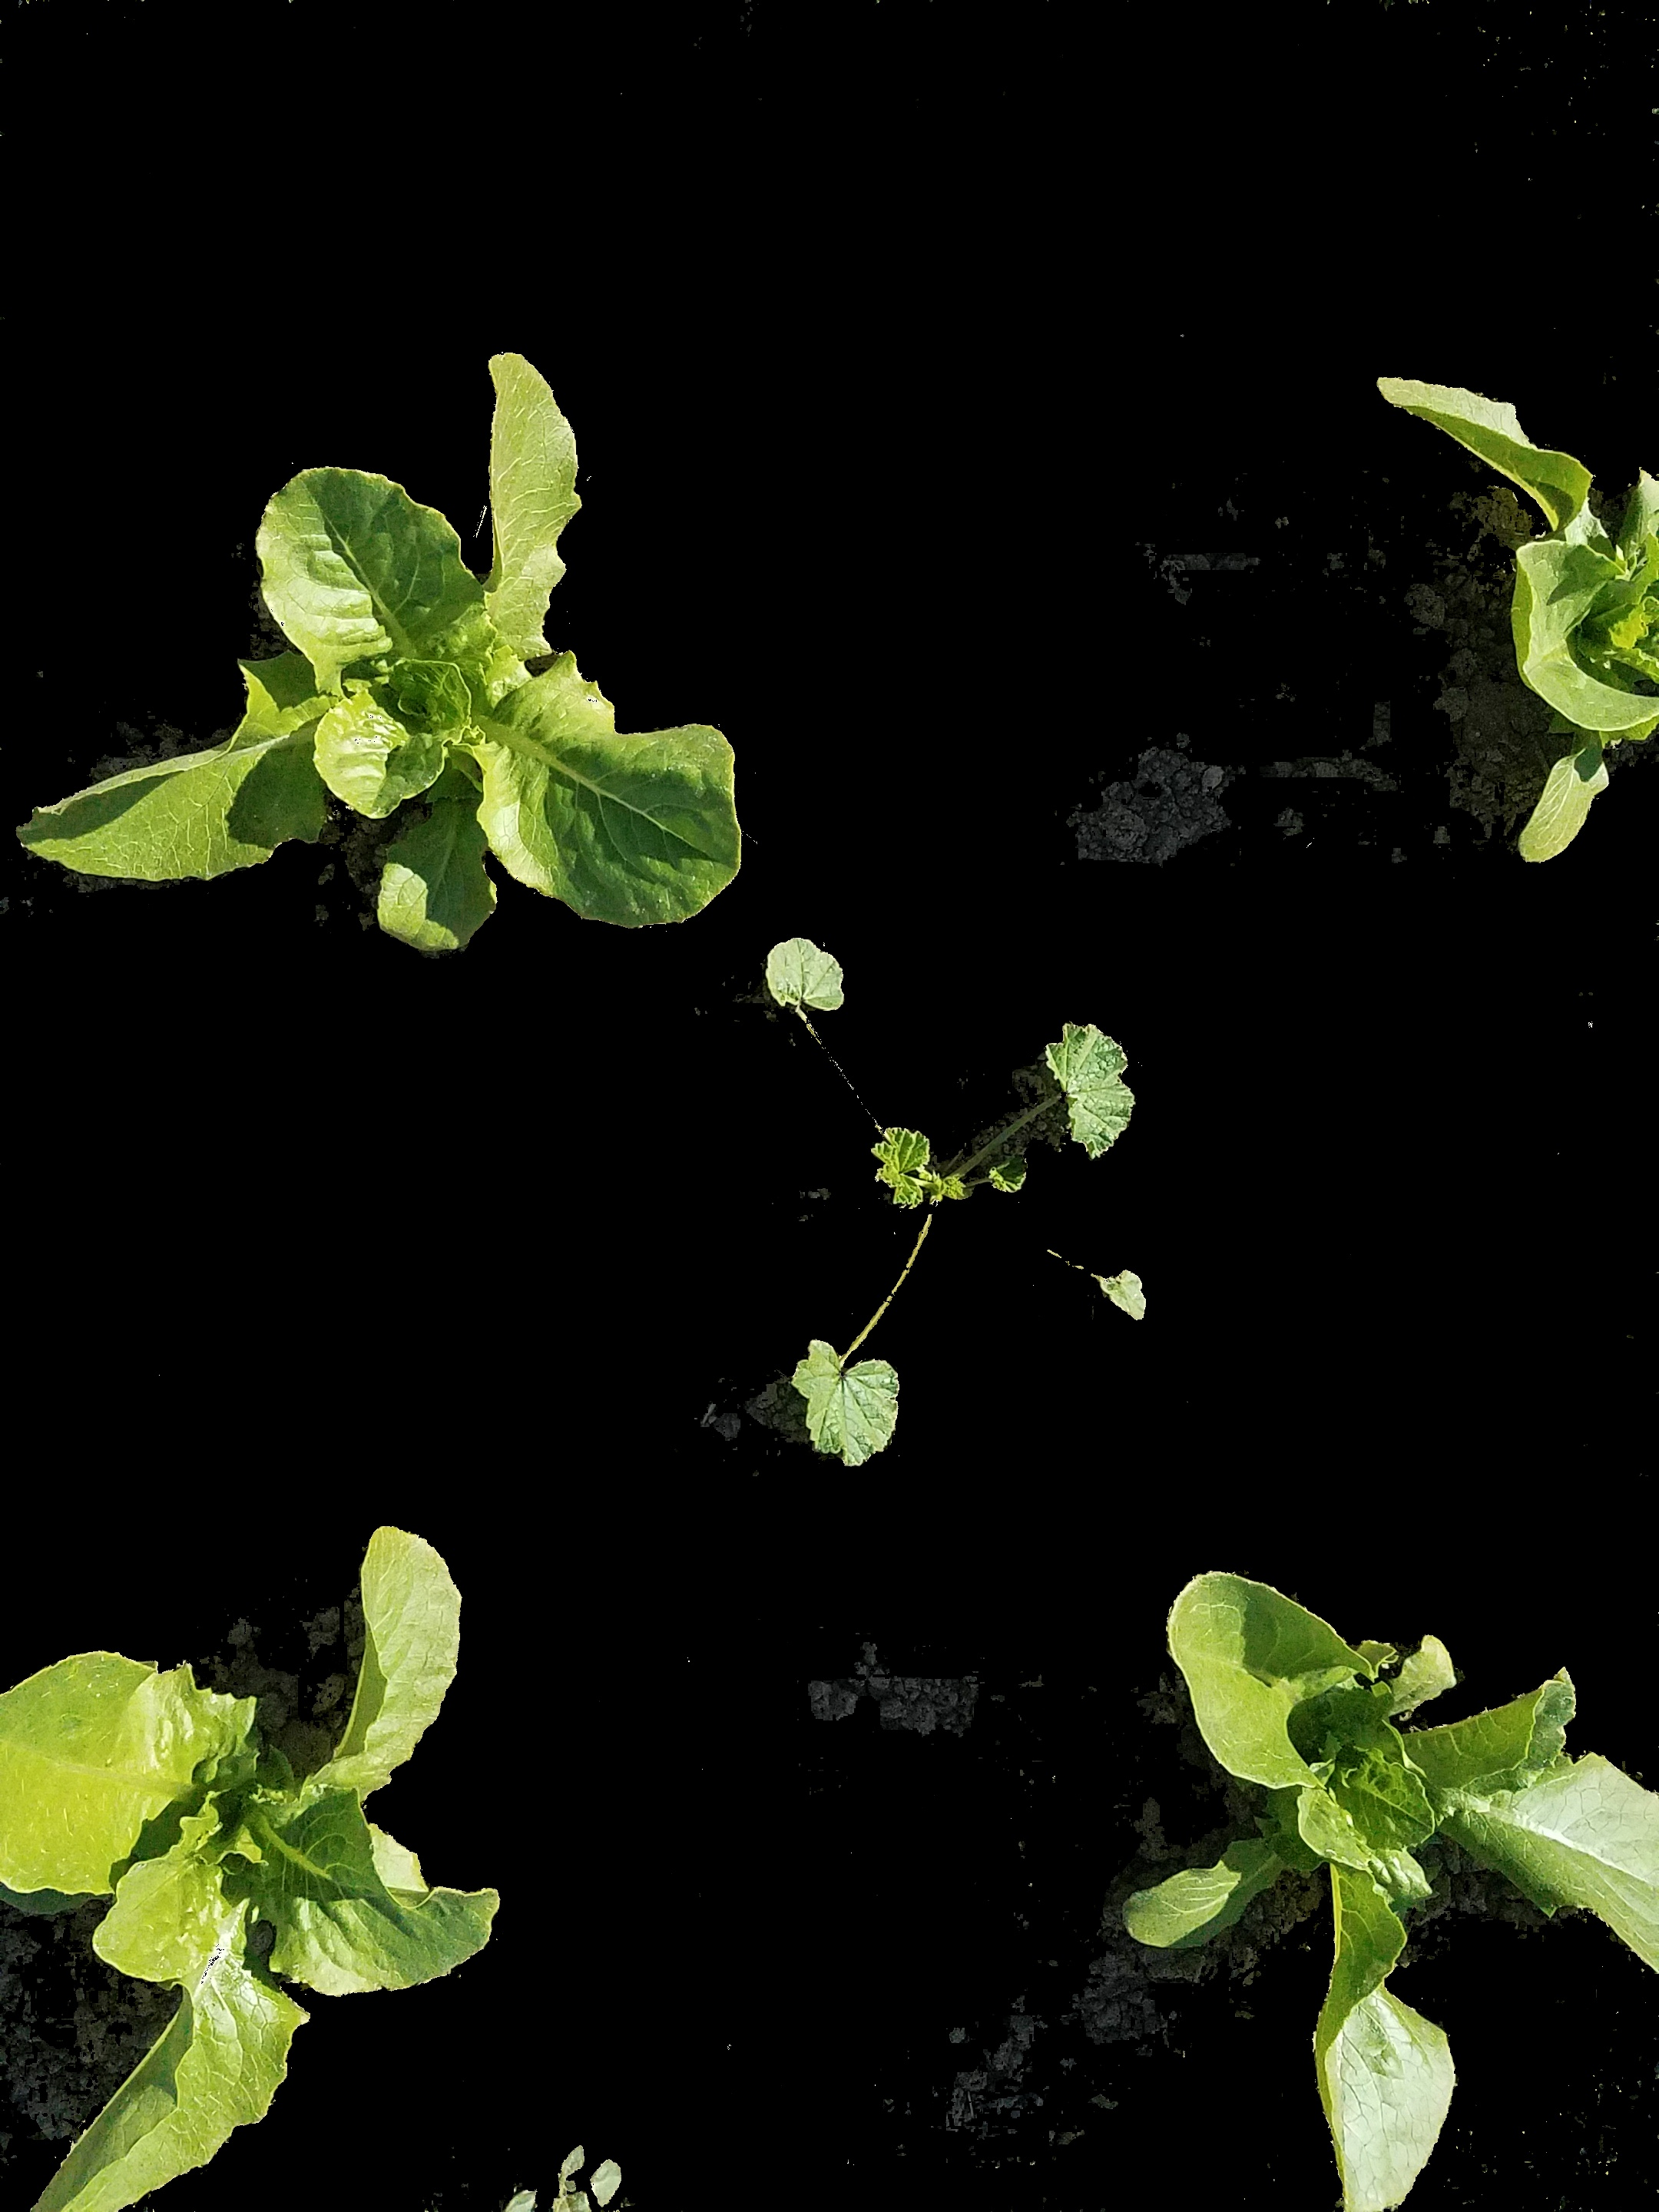
\includegraphics[width = 1.25in]{figures/20201117_112624-YCbCrI.jpg} \label{fig:ycbcr}} &
	\subfloat[YIQ]{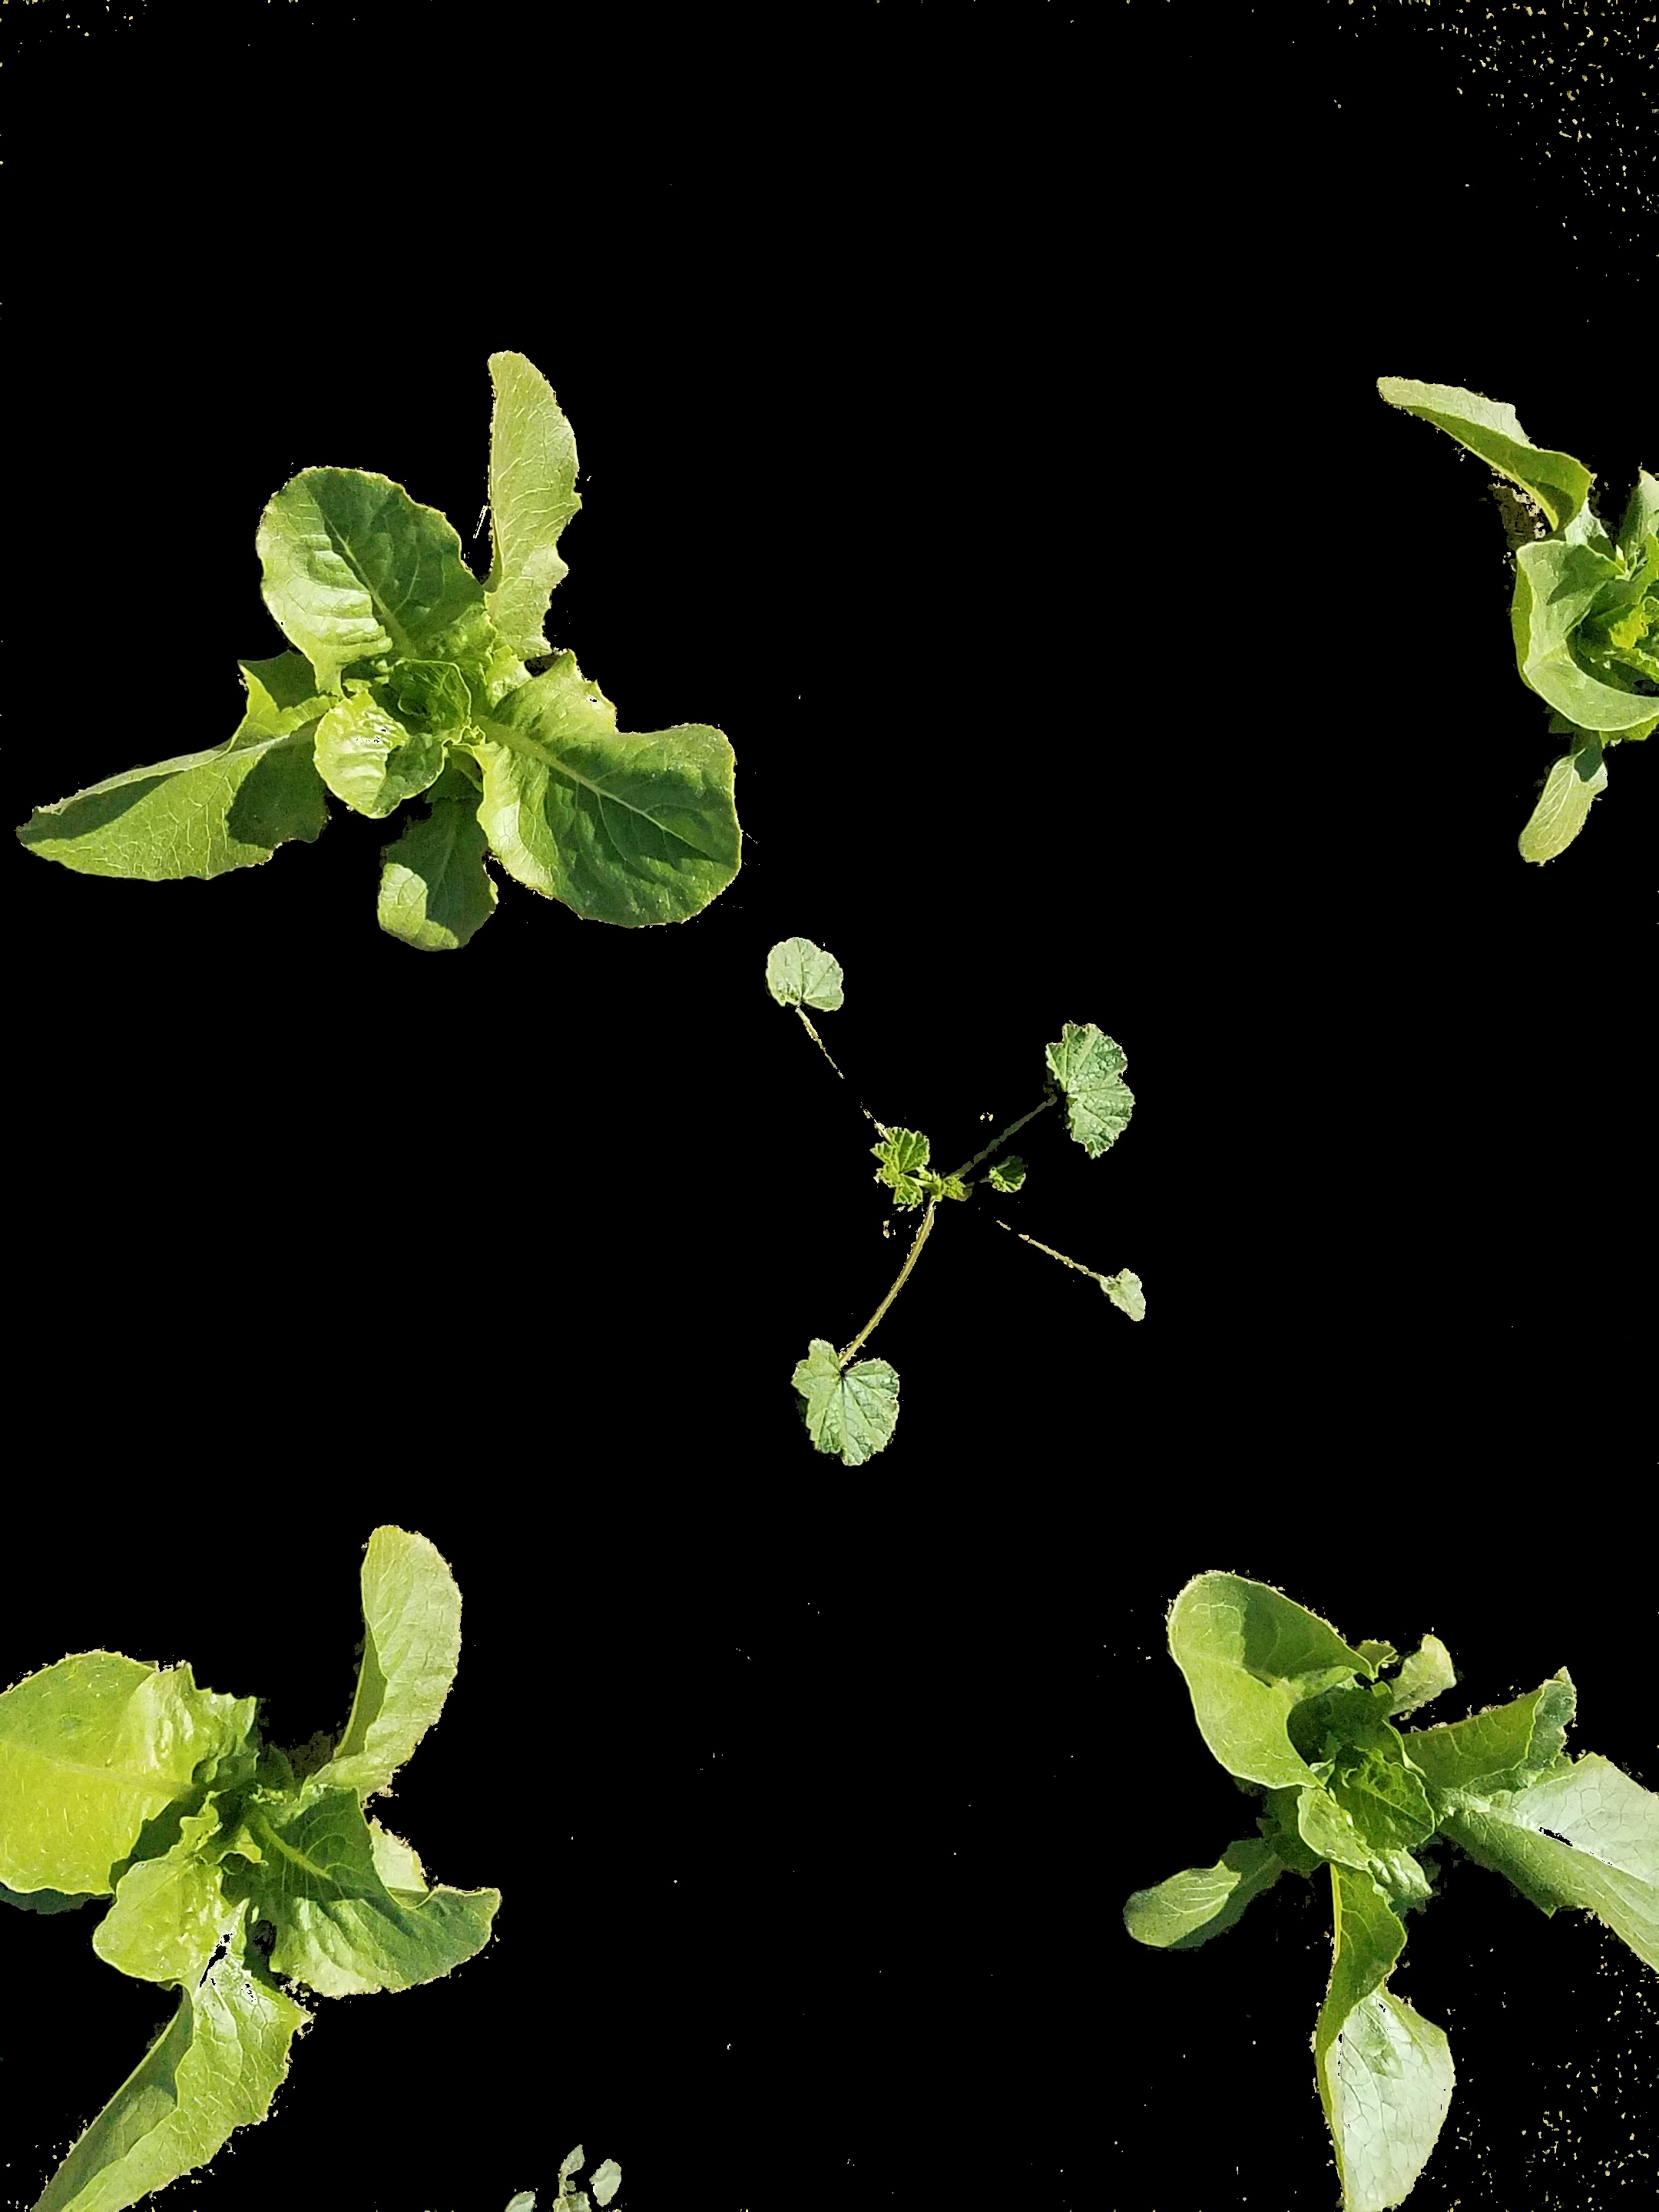
\includegraphics[width = 1.25in]{figures/20201117_112624-YI.jpg} \label{fig:yiq}} &
	\subfloat[Original]{\includegraphics[scale=0.0415,angle=270]{figures/20201117_112624.jpg} \label{fig:original}} \\
	\end{tabular}
	\caption[Segmentation results from various colorspaces outside RGB]{Segmentation results from various colorspaces outside RGB. The \ref{fig:ci} and \ref{fig:yiq} segmentation approaches are relatively clean, providing vegetation images that are free of ground clutter. The other three approaches, while providing good vegetation images, show too much of the ground, particularly in areas near to a plant, likely due to color contamination in the shadow area}
	\label{figure:results-colorspaces}
\end{figure}

\subsubsection{Problem: Reflections and Shadows}
Reflections within vegetation provide a challenge not easily surmounted.  In some cases, the area in reflection is not merely brighter than the surrounding pixels, but is completely devoid of usable pixels, as it is completely white (sometimes referenced as \textit{clipped}). This leads to the situation where portions of the vegetation are not present in the final segmented image, as the pixels do not contain the values associated with vegetation.  Deep shadows suffer from a problem similar to reflections in that they may be seen as nearly pure black. While mild shadows or reflections do not present much of a challenge, as vegetation in these areas typically have pixel values that are closely associated with their class. Reflections and shadows can be partially mitigated by a technique that improves the overall contrast of the image: histogram equalization. Histogram equalization, for lack of a more precise description, stretches out the contrast over a broad range. While histogram equalization cannot reconstruct pixels than have been registered as pure white or pure black.

% This produces figures that have aligned captions -- the [t] bit does the trick
\begin{figure*}[h]
	\centering
	\begin{subfigure}[t]{.24\textwidth}
	  \centering
	  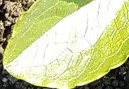
\includegraphics[width=.8\textwidth]{figures/reflection.jpg}
	  \caption{A leaf with reflection}
	  \label{fig:leaf-with-reflection}
	\end{subfigure}
	\begin{subfigure}[t]{.24\textwidth}
	  \centering
	  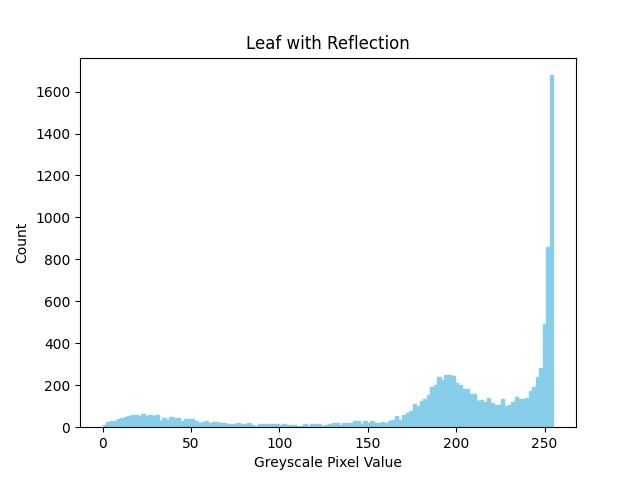
\includegraphics[width=.8\textwidth]{figures/reflection-histogram.jpg}
	  \caption{Before equalization}
	  \label{fig:reflection-histogram}
	\end{subfigure}
	\begin{subfigure}[t]{.24\textwidth}
	  \centering
	  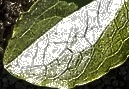
\includegraphics[width=.8\textwidth]{figures/reflection.equalized.jpg}
	  \caption{A leaf after equalization}
	  \label{fig:leaf-equalized}
	\end{subfigure}
	\begin{subfigure}[t]{.24\textwidth}
	  \centering
	  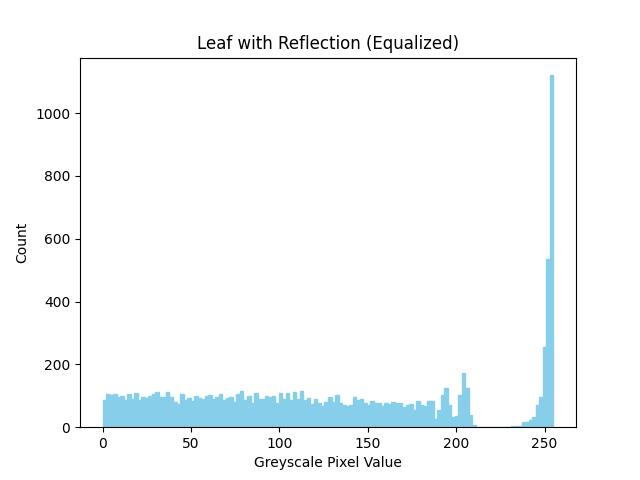
\includegraphics[width=.8\textwidth]{figures/reflection-histogram-equalized.jpg}
	  \caption{After equalization}
	  \label{fig:leaf-equalized-histogram}
	\end{subfigure}
	\caption[Reflection problems in segmented vegetation]{Reflections may be clipped (completely white) containing no usable information. While histogram equalization improves the image somewhat, applying that technique cannot reconstruct pixels that have been recorded as pure white. Figure~\ref{fig:leaf-with-reflection} shows a portion of an image with a reflection strong enough to render a significant portion of the image unusable. Note the pixel count for pure or nearly pure white pixels in both \ref{fig:reflection-histogram} and \ref{fig:leaf-equalized-histogram} remain constant.  Those pixels should contain values indicative of vegetation.}
	\label{fig:reflection}
\end{figure*}



\subsubsection{Color problems}
\label{section:problems-color}
Many of the indexes suffer from the same problem: they are focused on vegetation being green. Green stems and leaves are easily detected, but stems and leaves of other colors are not. Consider commonly encountered red-leaf lettuce. Depending on the stage of development and the angle of view, the leaves can be partially or entirely red (or a deep purple color). This is not limited to crops, of course, weeds such as redroot pigweed (\textit{Amaranthus retroflexus}) have red at the base of the leaves. Likewise, some weeds exhibit red stems. Purslane (\textit{Portulaca oleracea}) has red stems, and as an added complication, red edges on the leaves. Attempts to reveal the stems are complicated by the ground often containing a strong red coloration. Unfortunately, the band of color featured in the stems (red) is frequently found in the background (soil), so attempts to make the stems appear in the masked image are problematic, as this solution tends to bring unwanted ground pixels in the final image that contain hues found within the stems. The result of this is that the non-green portions of the vegetation does not appear in the resulting segmentation.  Even predominately green vegetation has non-green portions. Flowers are often missed by a green-centric index. While the omission of flowers may be desirable in further processing, if the flower obscures green vegetation that would otherwise be identified as such, that complicates further processing, especially when the green portion is significantly obscured. Uncorrected colors also complicate segmentation, as the same plant's leaves may be captured differently with two different cameras or under different lighting conditions. Under controlled lighting conditions (such as would be encountered in an enclosed system) color calibration is not essential every time, but systems that use ambient lighting require calibration each time to achieve optimal results. While the loss of red portions of the plant may not be a significant factor in subsequent processing, this should be taken into account. It may be the case that a single plant appears to be many more, as seen in \ref{fig:ndi}.
Even green portions of the vegetation may be green ``enough''. The segmented images in Figure~\ref{fig:result} have discarded ground pixels while retaining most of the vegetated pixels that will be used is subsequent processing, but a close examination reveals that pixels in the stems of the weed in the center are also eliminated, as they are less green than the rest of the plant. Likewise, immature vegetation where stems are not sufficiently green will not appear in the final image.

\begin{figure*}[h]
	\centering
	\begin{subfigure}[t]{.30\textwidth}
	  \centering
	  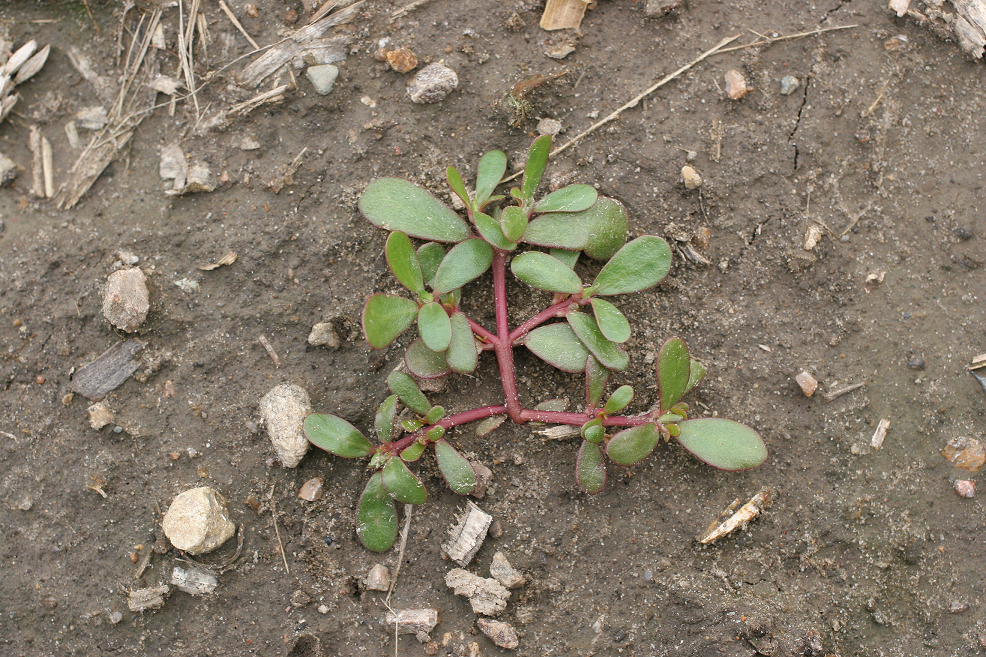
\includegraphics[width=1\linewidth]{figures/purslane.png}
	  \caption{Field view of Purslane}
	  \label{fig:original}
	\end{subfigure}
	\begin{subfigure}[t]{.30\textwidth}
	  \centering
	  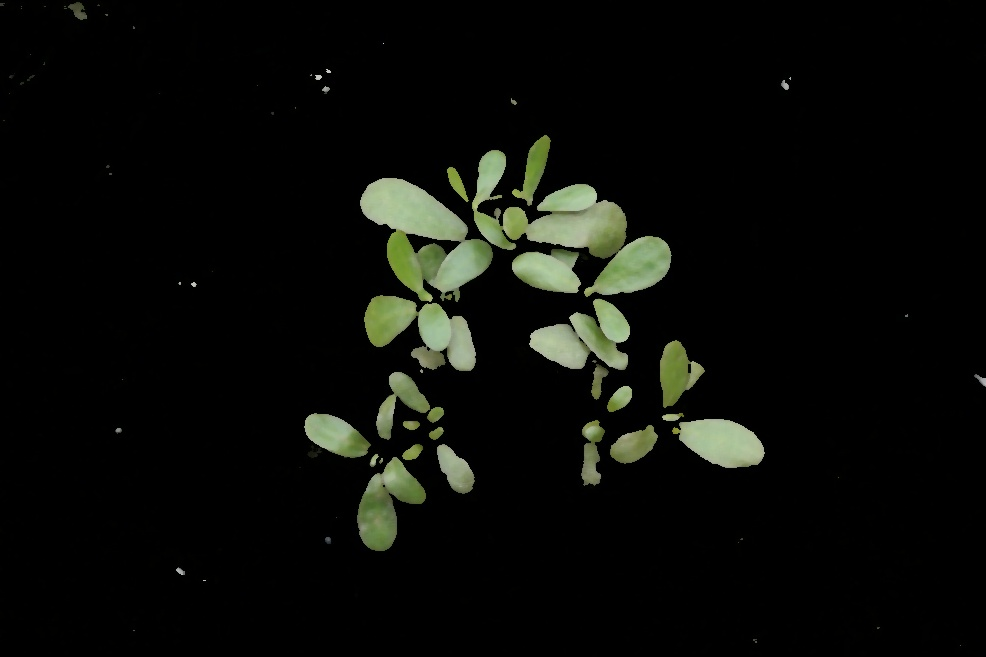
\includegraphics[width=1\linewidth]{figures/ndi-purslane.jpg}
	  \caption{Image processed with NDI}
	  \label{fig:ndi}
	\end{subfigure}
	% Bar chart produced with this command
	% python evaluate-masks.py -i c:\uofa\weeds\lib\testing\IMG_1133 -s c:\uofa\maricopa\corrected\2024-04-24\iphone-drip\IMG_1133.jpg -t d:\maricopa\masks\2024-04-24\IMG_1133-mask.jpg -l ..\jetson\logging.ini
	\begin{subfigure}[t]{.30\textwidth}
	 	\centering
	  	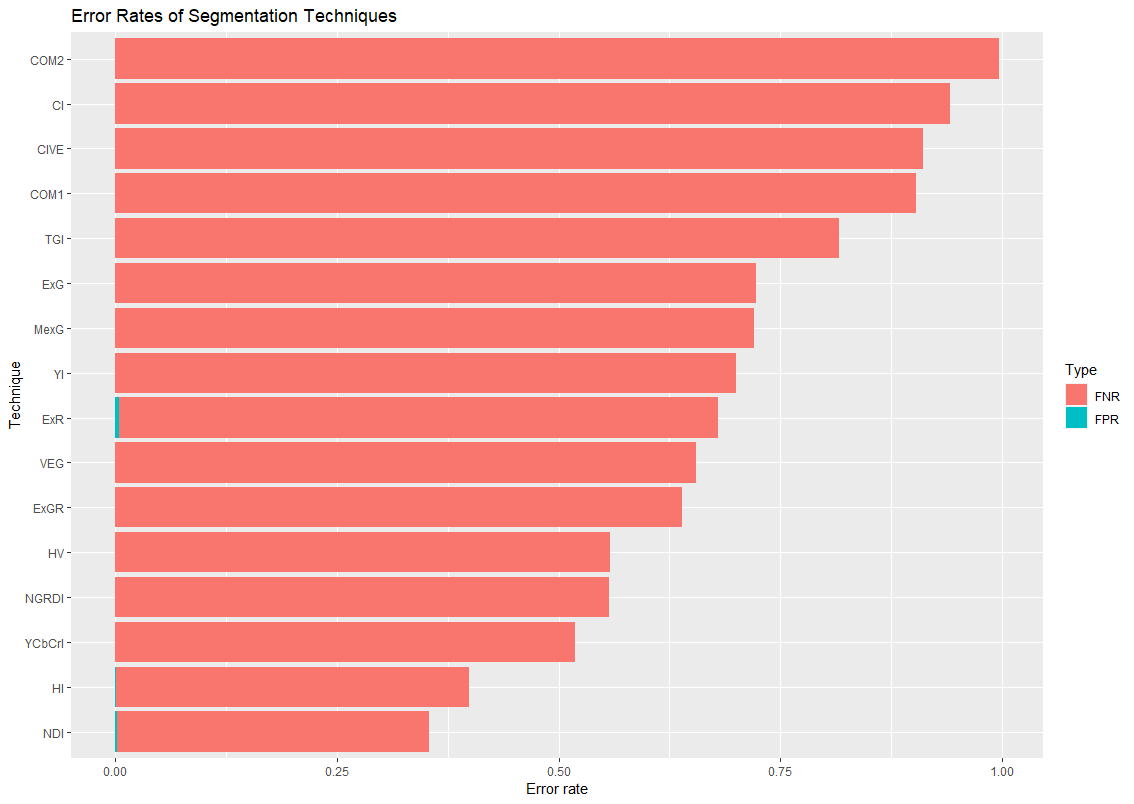
\includegraphics[width=1\linewidth]{figures/segmentation-error-rates-color.png}
	  	\caption{Error rates}
	  	\label{fig:error-rates}
	\end{subfigure}
	\caption[Missing red portions of vegetation]{The red portions of the vegetation are missing after the index has been applied, as ~\ref{fig:ndi} shows. While the absence of stems may not affect further image processing using factors like leaf texture in classification, the absence of the red portions of features such as leaves may complicate attempts to use factors that are affected such as shape. As \ref{fig:error-rates} shows, the presence of red in a significant portion of the vegetation has a negative impact on the error rates of the algorithms examined}
	\label{fig:segmentation}
\end{figure*}


% Correct equaliztion:
%  python manipulate.py -i ../../post-equalization/20201117_112624.jpg -o ../../post-equalization/equalized.jpg -e -l logging.ini
% Produce the masks:
%  python VegetationIndex.py -i ../../post-equalization/equalized.jpg -o ../../post-equalization
% Evaluate, and produce plot
%  python evaluate-masks.py -i ../lib/mask.jpg -t ../../post-equalization/equalized


\subsection{Classification Based}
\label{section:classification}
A different approach is to classify each of the pixels in an image as belonging to one of two classes: vegetation or ground (This is often referred to as \textit{semantic segmentation}) Table \ref{table:ml-segmentation} shows the results of building models using the following approaches:  Support Vector Machine, Linear Discriminant Analysis, and Multi-layer Perceptron (MLP). Each technique was applied to these color spaces: RGB, YIQ, YUV, HSI, HSV, YCbCr, and CIELab. A set of images taken from 2M AGL was selected and 20 samples taken from each of the 58 images, 10 ground points and 10 vegetation points. The term \textit{samples} in this context means that for each of the points sampled, the values for each of the color spaces identified in Section \ref{section:classification} were recorded. Based on these sample points, models were created and trained on 60\% of the data using the Scikit-learn Python library. While the RGB color space is commonly encountered, using it did not produce the best results for any of the techniques examined. That distinction tended to be -- but not always was -- the YIQ space. There are some important exceptions to keep in mind, particularly the performance of LDA, where identical scores for both RGB and YIQ spaces are seen. Using these classification approaches is not particularly pragmatic from a realtime perspective, as classifying every pixel in a modest 12MP image can take several hours on a modestly powerful CPU.\footnote{An approach optimized for a GPU would, no doubt, be much faster, but that is an exercise that is beyond the scope of this document}

%\subsubsection{Methods}
%Images were taken at the University of Arizona's Maricopa Agricultural Center (MAC) located in Maricopa, AZ (N 33.061857, E 111.967145) of a cantaloupe planting in May 2024. Images were obtained using a DJI Air 2S drone equipped with a standard RGB 20MP sensor for that model. These images were color corrected using values obtained from images taken under of a Datacolor Sypder correction chart. A set of images taken from 2M AGL was selected and 20 samples taken from each of the 58 images, 10 ground points and 10 vegetation points. The term \textit{samples} in this context means that for each of the points sampled, the values for each of the color spaces identified in Section \ref{section:classification} were recorded. Based on these sample points, models were created and trained on 60\% of the data using the Scikit-learn Python library.

%
% Begin Copied Table from this command
% python segment.py -i images -o segmented -t ../util/segmentation-training.csv  -b -s -l logging.ini -a all
% Minor manual edit: Remove leading space from header lines

Table \ref{table:ml-segmentation} shows a summary of the three classification approaches in various color spaces, giving the Area Under the Curve (AUC), Precision, Recall, and F1 scores. And while the the scores reported are encouraging, the resulting segmented images are not.

% Spacing between the rows
\renewcommand*{\arraystretch}{1.1}

%
% Begin Copied Table from this command
% python segment.py -i images -o segmented -t ../util/segmentation-training.csv  -b -s -l logging.ini -a all
% Minor manual edit: Remove leading space from header lines & data


\begin{longtable}{llrrrr}
\caption[Machine Learning Segmentation]{Machine Learning Segmentation}
\label{table:ml-segmentation}\\
\toprule
Technique &  Color &  AUC & Precision & Recall &   F1 \\
\midrule
\endfirsthead
\caption[]{Machine Learning Segmentation} \\
\toprule
Technique &  Color &  AUC & Precision & Recall &   F1 \\
\midrule
\endhead
\midrule
\multicolumn{6}{r}{{Continued on next page}} \\
\midrule
\endfoot

\bottomrule
\endlastfoot
MLP &RGB & 0.93 &      0.88 &   0.95 & 0.91 \\
MLP &YIQ & 0.94 &      0.88 &   0.96 & 0.92 \\
MLP &YUV & 0.94 &      0.88 &   0.96 & 0.92 \\
MLP &HSI & 0.91 &      0.86 &   0.94 & 0.90 \\
MLP &HSV & 0.90 &      0.87 &   0.94 & 0.91 \\
MLP &YCBCR & 0.94 &      0.88 &   0.96 & 0.92 \\
MLP &CIELAB & 0.94 &      0.88 &   0.96 & 0.92 \\
LDA &RGB & 0.94 &      0.88 &   0.96 & 0.92 \\
LDA &YIQ & 0.94 &      0.88 &   0.96 & 0.92 \\
LDA &YUV & 0.94 &      0.88 &   0.96 & 0.92 \\
LDA &HSI & 0.91 &      0.86 &   0.95 & 0.90 \\
LDA &HSV & 0.90 &      0.86 &   0.95 & 0.90 \\
LDA &YCBCR & 0.94 &      0.88 &   0.96 & 0.92 \\
LDA &CIELAB & 0.94 &      0.88 &   0.96 & 0.92 \\
SVM &RGB & 0.94 &      0.89 &   0.96 & 0.92 \\
SVM &YIQ & 0.92 &      0.88 &   0.82 & 0.85 \\
SVM &YUV & 0.93 &      0.86 &   0.93 & 0.89 \\
SVM &HSI & 0.91 &      0.87 &   0.94 & 0.90 \\
SVM &HSV & 0.90 &      0.87 &   0.94 & 0.90 \\
SVM &YCBCR & 0.92 &      0.85 &   0.91 & 0.88 \\
SVM &CIELAB & 0.91 &      0.86 &   0.96 & 0.90 \\
\end{longtable}

% 
% End copied table
%
\subsection{Semantic Segmentation}
Semantic segmentation is a convolutional neural network (CNN) using a trained model to classify each pixel in an image with a class label.  For the most part, agricultural images contain only two things: plants and the ground. While there are exceptions to this, of course, as images may include debris on the ground, irrigation equipment, etc., but from another viewpoint, images contain pixels that are plants and pixels that aren't.  The focus here is not to actually classify what each pixel represents (a brocolli plant, a segment of pipe, the ground, etc.), but to produce a mask that can be applied to the image to isolate vegetated pixels. This approach differs from the prior two approaches in that while index-based approaches consider no information about other images, and learning base approaches consider samples of a set of images to predict class membership, the deep-learning techniques considered in this section are trained on both images and the corresponding masks.

\subsubsection{U-Net}
The name of the U-Net architecture derives from the U-shaped arrangement of the downard decoder section and the upward encoder section. Developed initially for the segmentation of bio-medical images \parencite{Ronneberger2015-ye}, this technique has been more widely adopted into various use cases.

\begin{figure}[H]
	\centering
	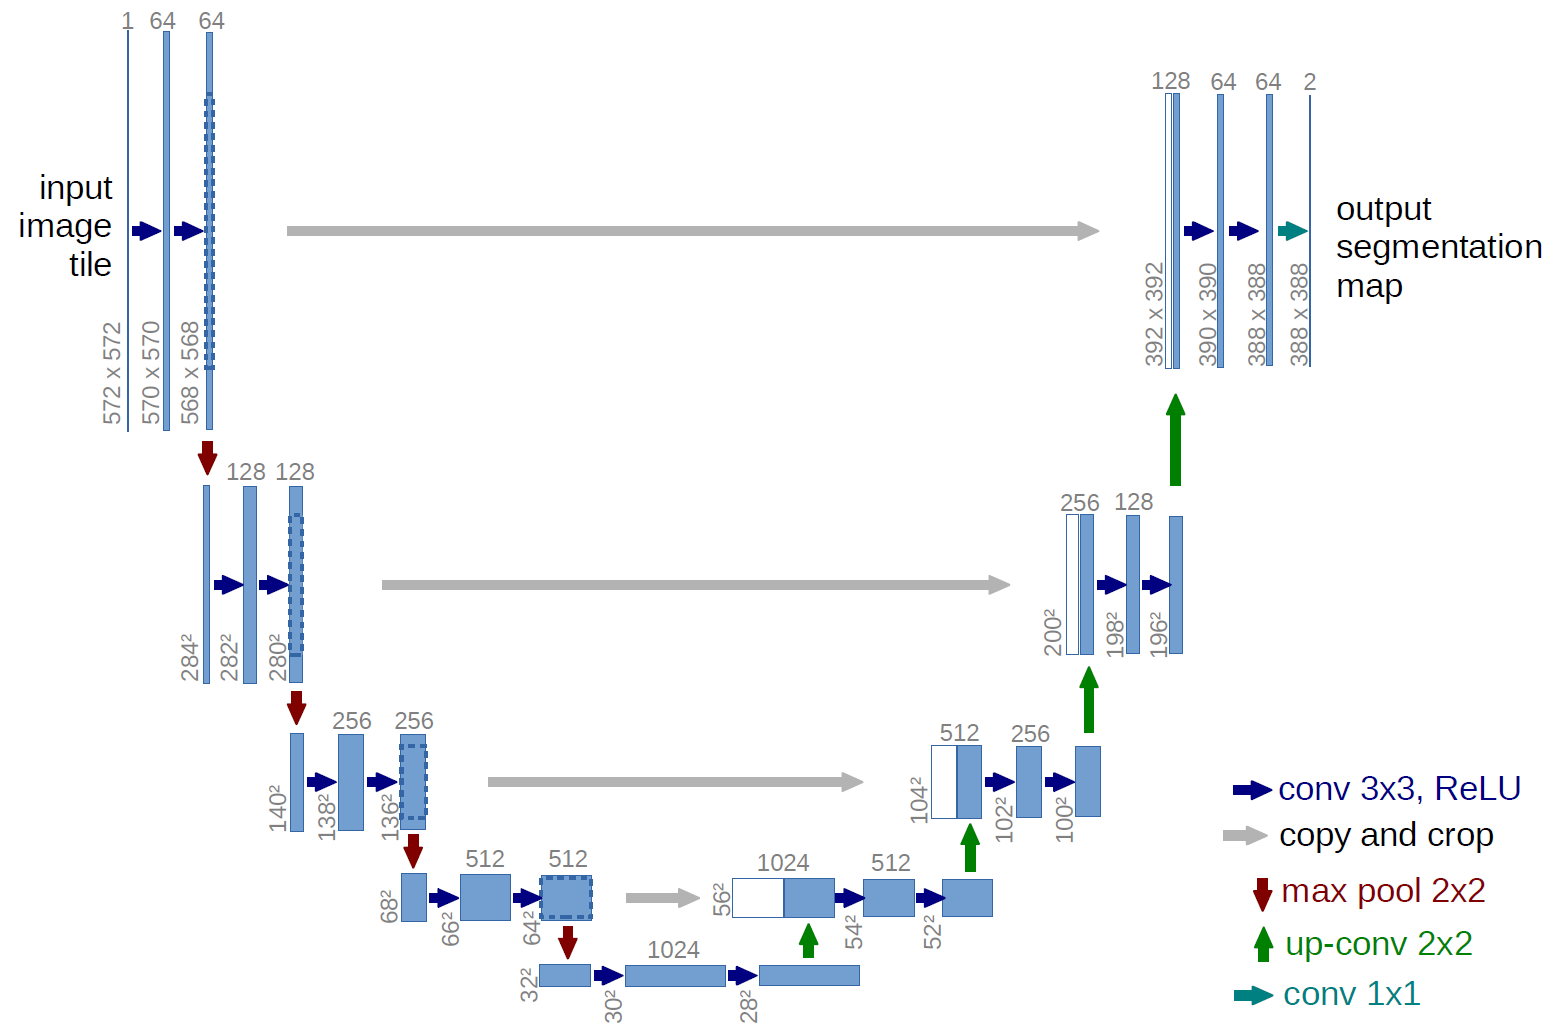
\includegraphics[height=5cm]{./figures/u-net-architecture.png}
	\caption{Image segmented using NDI}
	\label{fig:u-net}
	\caption[U-Net architecture]{The name of U-Net architecture refers to the arrancement of decoders (often referred to as a contracting path) and encoders (the expanding path)}
\end{figure}
This architecture has a bit of a limitation that must be taken into acount in image sets: the length of each image's axis must be a mutiple of 32. That is, a 32x32 image will work, but a 32x90 image will not. The images and masked used for training and testing should be resized to fit this limitation. Using a model trained on images and associated masks from the MAC to a set of test images yields fairly low error rate masks when  those masks are evaluated against the ground truth: FPR of 0.0005 and FNR of 0.06, comparable to the lower rates achieved with some index-based approaches.

\begin{figure}[H]
	\centering
	\begin{subfigure}[h]{.30\textwidth}
	  \centering
	  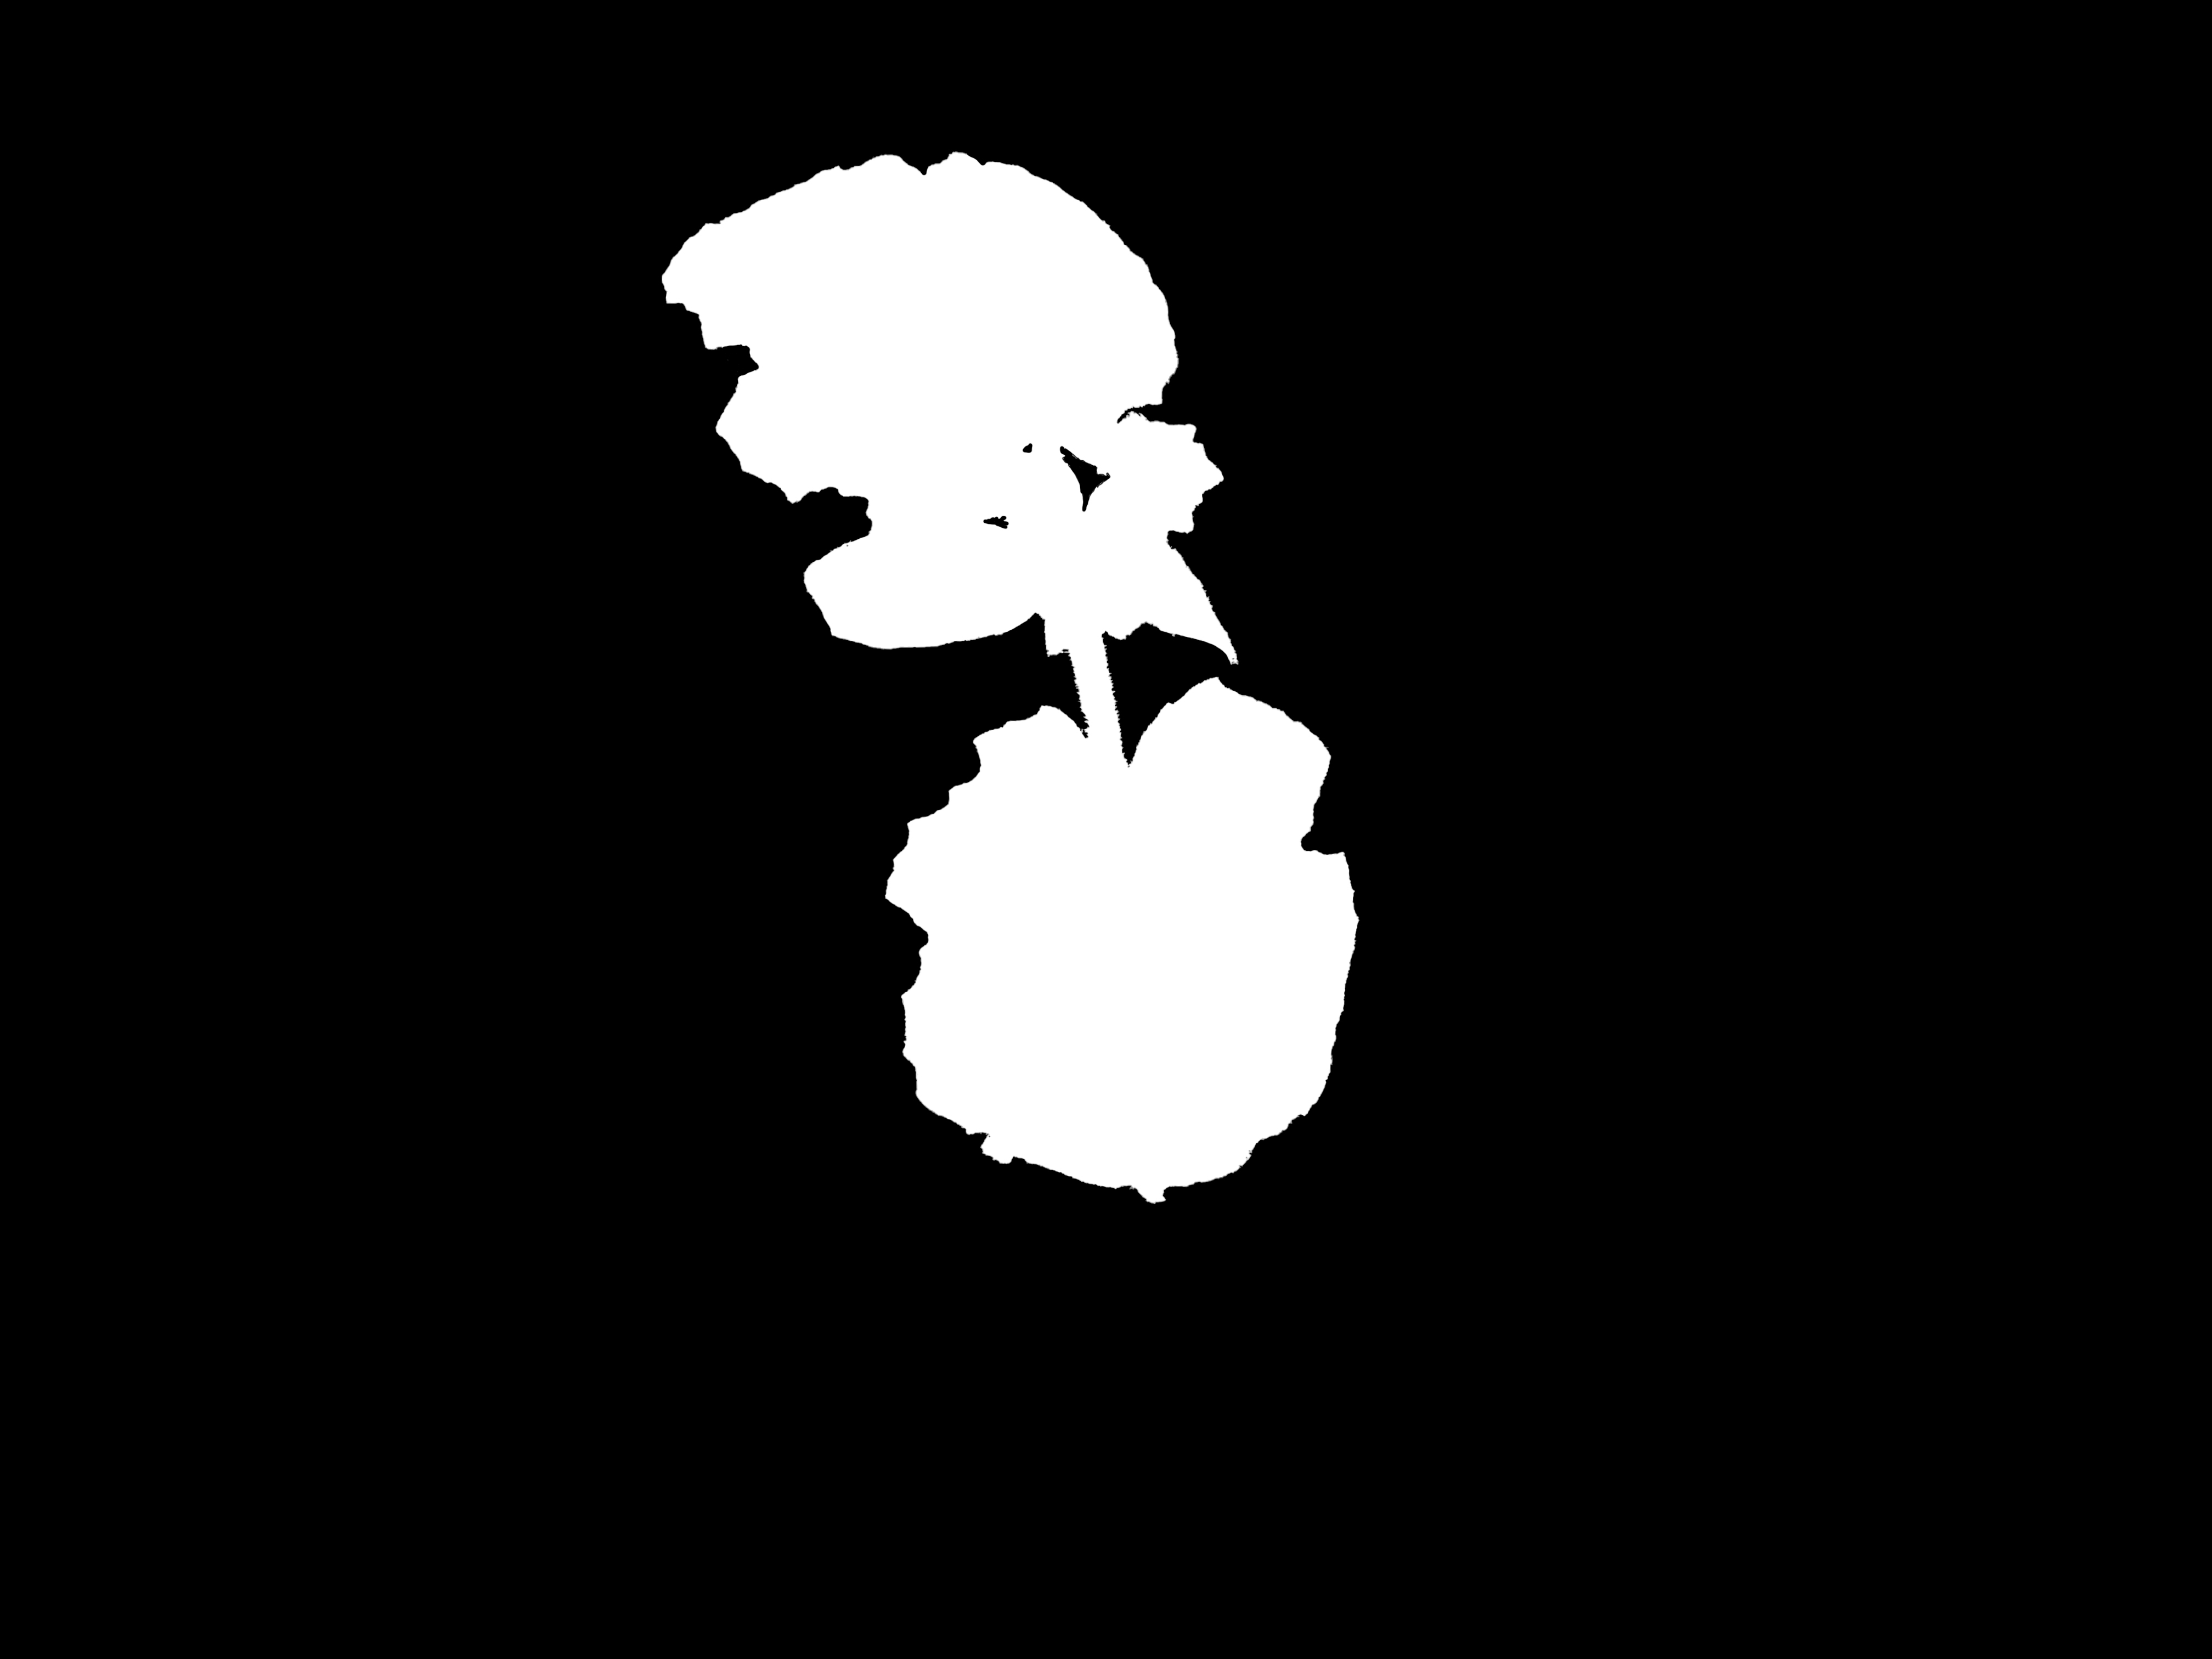
\includegraphics[width=1\linewidth]{figures/IMG_1115-mask.jpg}
	  \caption{Ground truth mask}
	  \label{fig:original}
	\end{subfigure}
	\begin{subfigure}[h]{.30\textwidth}
	  \centering
	  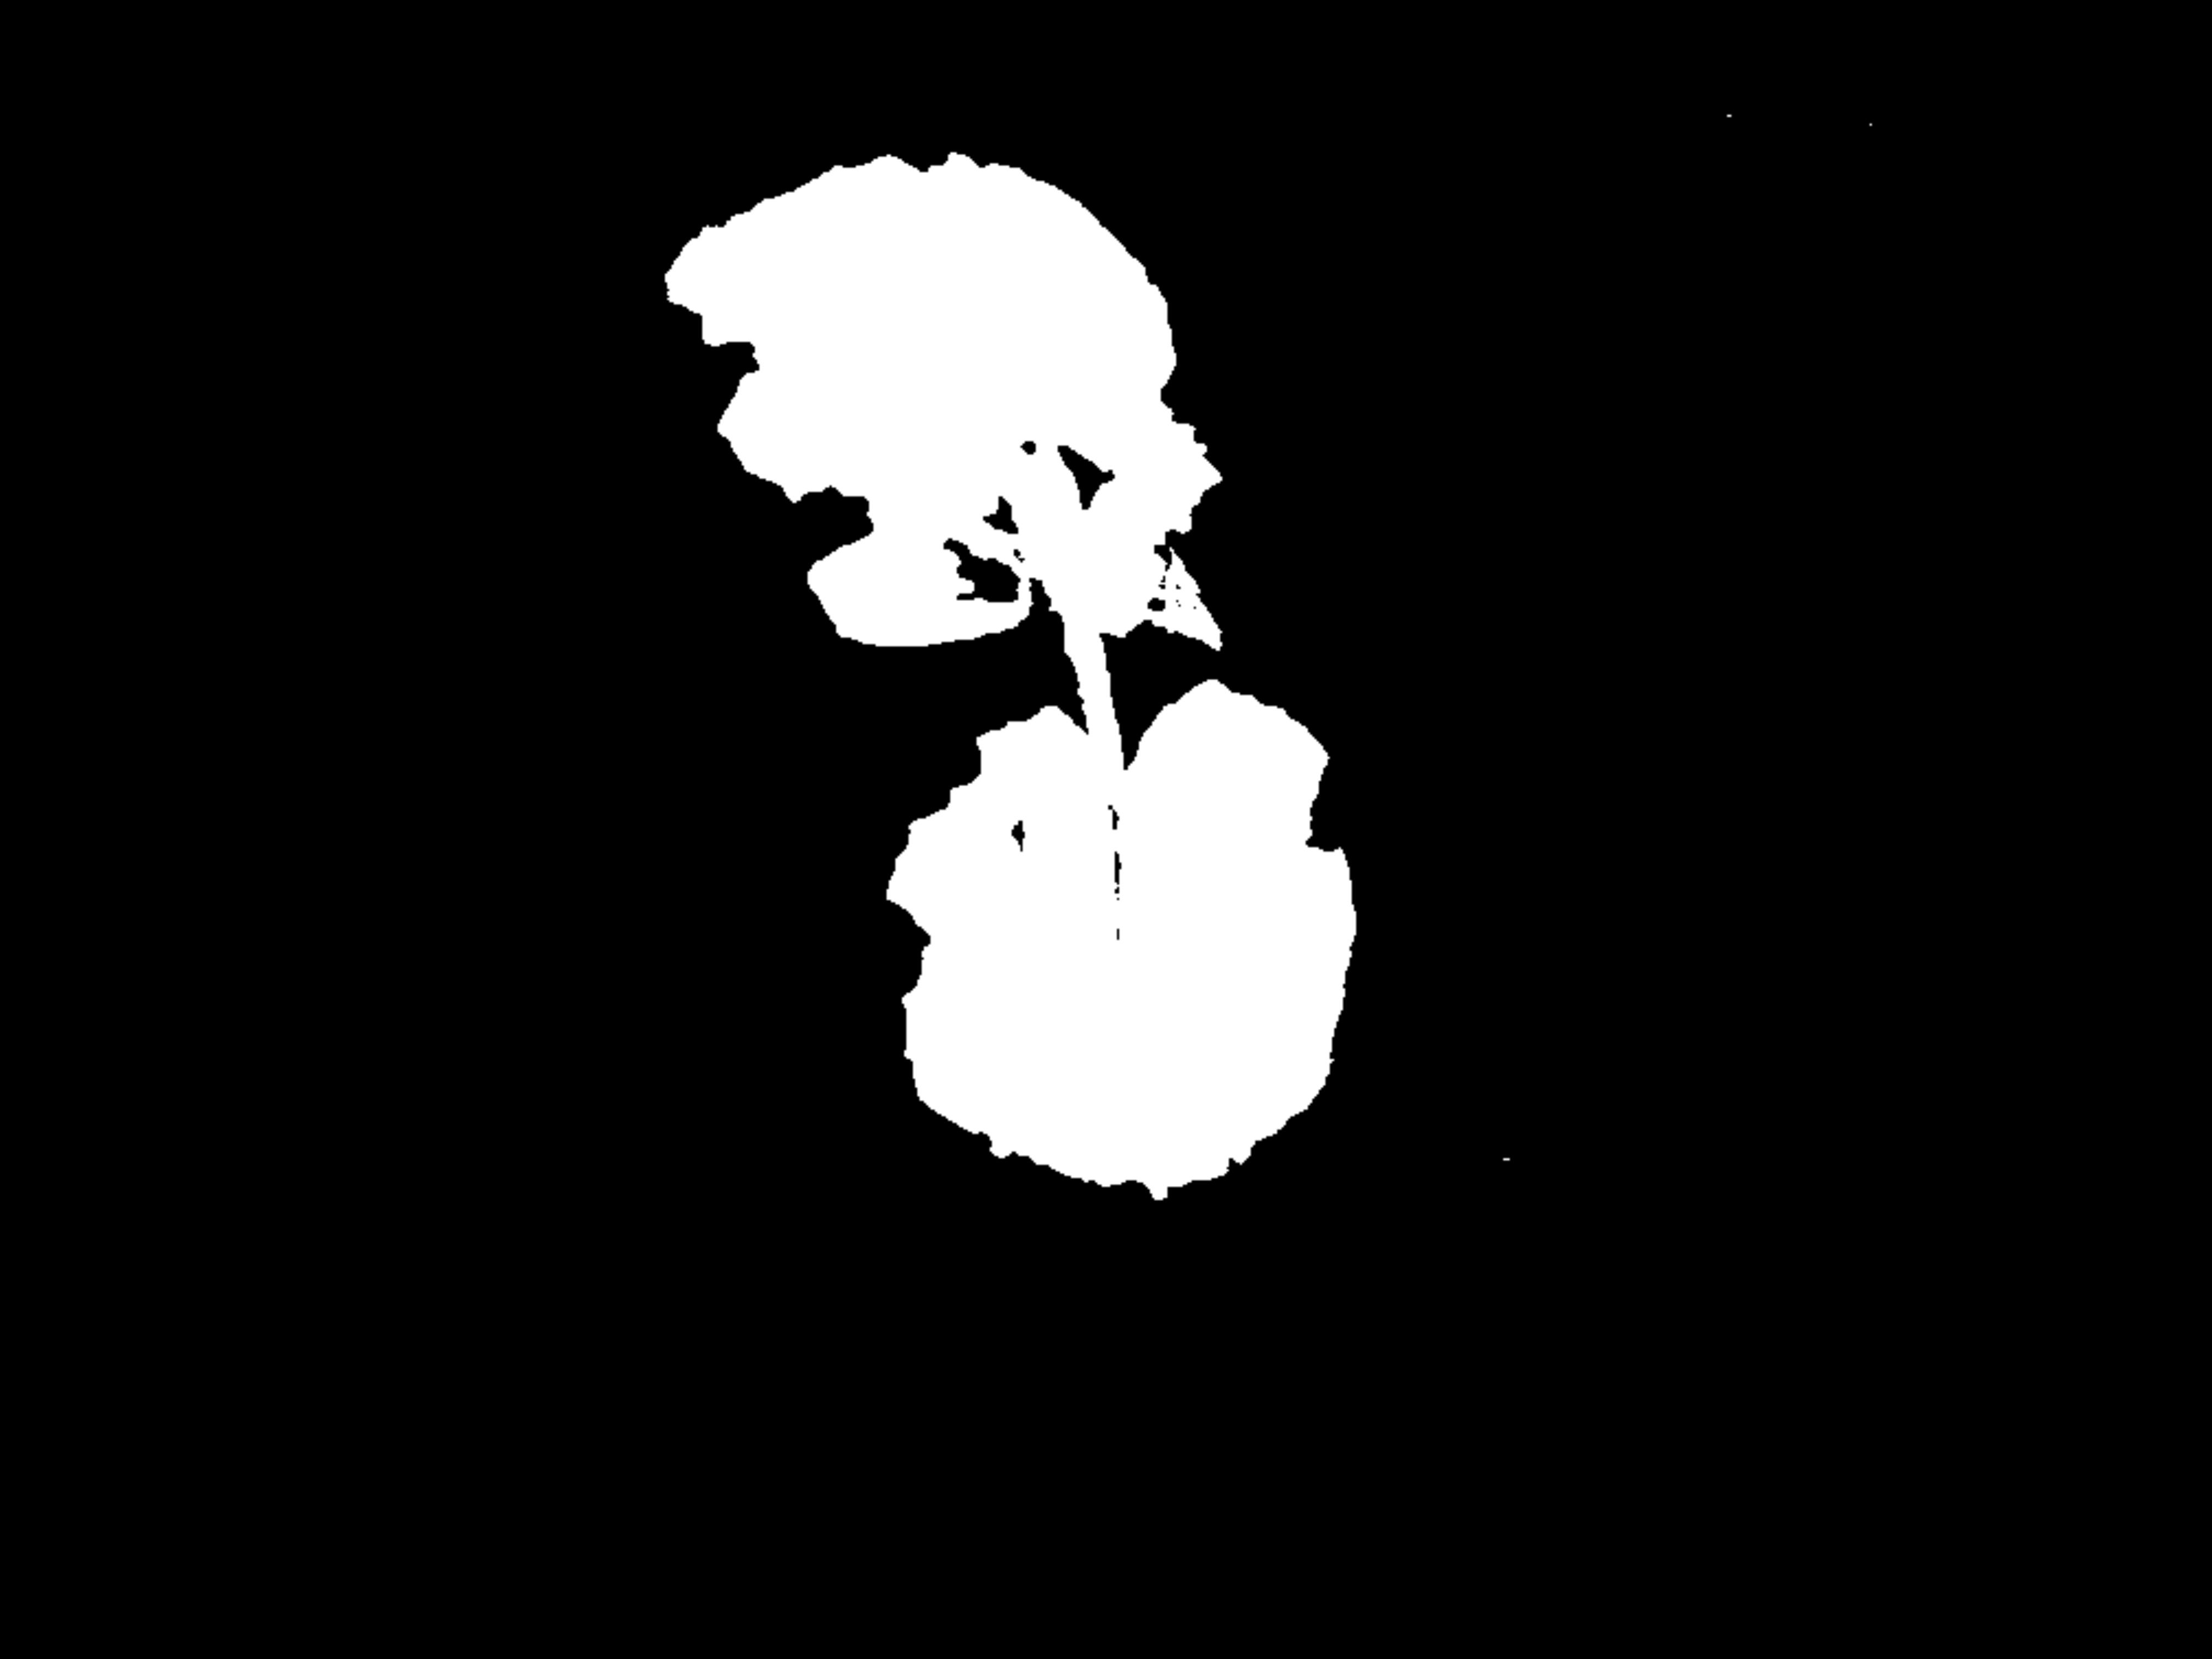
\includegraphics[width=1\linewidth]{figures/IMG_1115-mask-unet.png}
	  \caption{Mask produced with U-Net}
	  \label{fig:mask}
	\end{subfigure}
	\begin{subfigure}[h]{.30\textwidth}
	  \centering
	  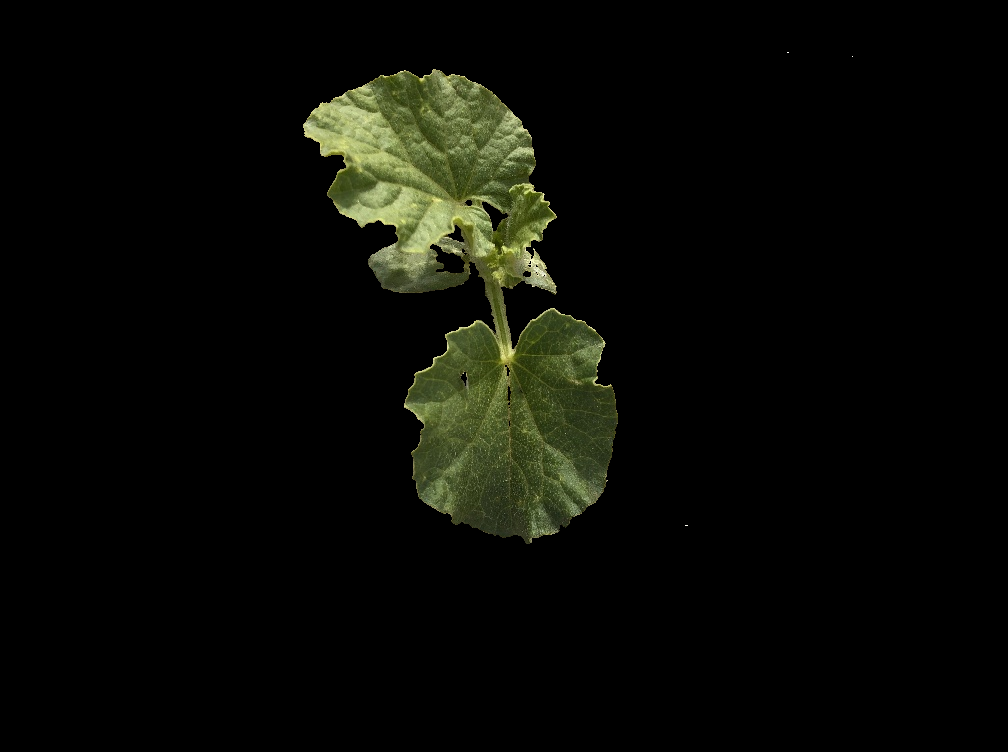
\includegraphics[width=1\linewidth]{figures/IMG_1115-original-masked.png}
	  \caption{After applying SegNet mask}
	  \label{fig:original-masked}
	\end{subfigure}
	\caption[U-Net segmentation vs ground truth]{The mask produced with U-Net shows some errors within the leaf, but is quite close to a match for the ground truth.}
	\label{fig:segmentation}
\end{figure}


%\section{Performance}
%\label{section:performance}
%The segmentation was performed it this environment:
%\begin{enumerate}
%	\item{HP Desktop -- TODO: Need model}
%	\item{64GB RAM}
%	\item{Python 3.10}
%	\item{Scikit-Learn 1.1.2}
%	\item{numpy 1.19.5}
%\end{enumerate}
%The classification of individual pixels is several orders of magnitude greater than VI based approaches. While an index for an image can be calculated in 10s of millisecond, classifying every pixel in an image takes much longer, many 10s of seconds.
%\section{Problems}
%\subsection{Index Based}
%\subsubsection{Reflections}
%
%
%\subsection{Classification Based}
%The most obvious problem with the classification based approach is performance, and while there are a few solutions to that that were discussed in Section \ref{section:performance}, but will not be repeated here. The classification approach also suffers 


\newpage
\section{References}
\printbibliography[heading=none]

%\cite{Wirth2004-li}
\end{document}

